%%%%%%%%%%%%%%%%%%%%%%%%%%%%%%%%%%%%%%%%%%%%%%%%%%%%%%%%%%%%%%%%%%%%%%
% LaTeX Template: Project Titlepage
%
% Source: http://www.howtotex.com
% Date: April 2011
% 
% This is a title page template which be used for articles & reports.
% 
% Feel free to distribute this example, but please keep the referral
% to howtotex.com
% 
%%%%%%%%%%%%%%%%%%%%%%%%%%%%%%%%%%%%%%%%%%%%%%%%%%%%%%%%%%%%%%%%%%%%%%
% How to use writeLaTeX: 
%s
% You edit the source code here on the left, and the preview on the
% right shows you the result within a few seconds.
%
% Bookmark this page and share the URL with your co-authors. They can
% edit at the same time!
%
% You can upload figures, bibliographies, custom classes and
% styles using the files menu.
%
% If you're new to LaTeX, the wikibook is a great place to start:
% http://en.wikibooks.org/wiki/LaTeX
%
%%%%%%%%%%%%%%%%%%%%%%%%%%%%%%%%%%%%%%%%%%%%%%%%%%%%%%%%%%%%%%%%%%%%%%
%
% --------------------------------------------------------------------
% Preamble
% --------------------------------------------------------------------
\documentclass[paper=a4, fontsize=10pt]{scrartcl}	% KOMA
\usepackage[bottom=1.1in, top=0.9in]{geometry}
\usepackage{lmodern}

\newcommand{\specialcell}[2][c]{%
	\begin{tabular}[#1]{@{}c@{}}#2\end{tabular}}
\usepackage{todonotes}
\usepackage{listings}
\usepackage{graphbox}
\usepackage{hyperref}
\usepackage{twoopt}
\usepackage{adjustbox}
\usepackage[english]{babel}
\usepackage{graphicx}
\usepackage{subcaption}
\usepackage{pgfplots}
\usepackage{mwe}
\usepackage{color, colortbl}
\usepackage[protrusion=true,expansion=true]{microtype}	
\usepackage{amsmath,amsfonts,amsthm,amssymb}
\usepackage{tabularx}
\usepackage{float}

\usepackage{lmodern}
\usepackage{amsmath}
\usepackage{todonotes}
\usepackage{listings}
\usepackage{graphbox}
\usepackage{hyperref}
\usepackage{twoopt}
\usepackage{adjustbox}
\usepackage[english]{babel}
\usepackage{graphicx}
\usepackage{subcaption}
\usepackage{mwe}
\usepackage{color, colortbl}
\usepackage[protrusion=true,expansion=true]{microtype}	
\usepackage{amsmath,amsfonts,amsthm,amssymb}
\usepackage{tabularx}
\usepackage{float}
\usepackage{tikz} 
\usepackage{xcolor}
\usepackage{listings}
\usepackage{arydshln}
\usepackage{bytefield}

\definecolor{mGreen}{rgb}{0,0.6,0}
\definecolor{mGray}{rgb}{0.5,0.5,0.5}
\definecolor{mPurple}{rgb}{0.58,0,0.82}
\definecolor{backgroundColour}{rgb}{0.95,0.95,0.92}

\newcommand\setrow[1]{\gdef\rowmac{#1}#1\ignorespaces}
\newcommand\clearrow{\global\let\rowmac\relax}
\usepackage{graphicx}
\usepackage[T1]{fontenc}
\definecolor{Red}{rgb}{1,0.7,0.7}
\definecolor{Yellow}{HTML}{FAFAD2}
\definecolor{Green}{HTML}{9ACD32}
\definecolor{Blue}{rgb}{0.5,0.8,1}
\lstset{
	frame=single,
	xleftmargin=15pt,
	xrightmargin=15pt,
	basicstyle=\ttfamily\small
}
\lstdefinestyle{CStyle}{
	backgroundcolor=\color{backgroundColour},   
	commentstyle=\color{mGreen},
	keywordstyle=\color{magenta},
	numberstyle=\tiny\color{mGray},
	stringstyle=\color{mPurple},
	basicstyle=\footnotesize,
	breakatwhitespace=false,         
	breaklines=false,                 
	captionpos=b,                    
	keepspaces=true,                 
	numbers=left,                    
	numbersep=5pt,                  
	showspaces=false,                
	showstringspaces=false,
	showtabs=false,                  
	tabsize=2,
	language=C
}
\lstset{basicstyle=\ttfamily,
	showstringspaces=false,
	commentstyle=\color{red},
	keywordstyle=\color{blue}
}


\usepackage{graphicx}
\usepackage[T1]{fontenc}
\definecolor{Red}{rgb}{1,0.7,0.7}
\definecolor{Yellow}{HTML}{FAFAD2}
\definecolor{Green}{HTML}{9ACD32}
\definecolor{Blue}{rgb}{0.5,0.8,1}
\lstset{
	backgroundcolor=\color{backgroundColour},   
	commentstyle=\color{mGreen},
	keywordstyle=\color{magenta},
	numberstyle=\tiny\color{mGray},
	stringstyle=\color{mPurple},
	basicstyle=\footnotesize,
	breakatwhitespace=false,         
	breaklines=false,                 
	captionpos=b,                    
	keepspaces=true,                 
	numbers=left,                    
	numbersep=5pt,                  
	showspaces=false,                
	showstringspaces=false,
	showtabs=false,                  
	tabsize=2,
	frame=single,
	xleftmargin=15pt,
	xrightmargin=15pt,
	basicstyle=\ttfamily\small
}
% --------------------------------------------------------------------
% Definitions (do not change this)
% --------------------------------------------------------------------
\newcommand{\HRule}[1]{\rule{\linewidth}{#1}} 	% Horizontal rule
\newcommandtwoopt*{\myref}[3][][]{%
	\hyperref[{#3}]{%
		\ifx\\#1\\%
		\else
		#1~%
		\fi
		\ref*{#3}%
		\ifx\\#2\\%
		\else
		\,#2%
		\fi
	}%
}

\makeatletter							% Title
\def\printtitle{%						
	{\centering \@title\par}}
\makeatother									

\makeatletter							% Author
\def\printauthor{%					
	{\centering \large \@author}}				
\makeatother							

% --------------------------------------------------------------------
% Metadata (Change this)
% --------------------------------------------------------------------
\title{	\normalsize \textsc{Politecnico di Torino\\GPU Programming} 	% Subtitle
	\\[2.0cm]								% 2cm spacing
	\HRule{0.5pt} \\						% Upper rule
	\LARGE \textbf{\uppercase{Report: PROJECT\\Webcam streaming \& filters}}	% Title
	\HRule{2pt} \\ [0.5cm]		% Lower rule + 0.5cm spacing
	\normalsize 
	\today % Todays date
}

\author{
	Matteo Battilana, Salvatore Gabriele La Greca, Giovanni Pollo
}

\begin{document}
	% ------------------------------------------------------------------------------
	% Maketitle
	% ------------------------------------------------------------------------------
	\thispagestyle{empty}		% Remove page numbering on this page
	
	\printtitle					% Print the title data as defined above
	\vfill
	\printauthor				% Print the author data as defined above
	\newpage


	\thispagestyle{empty}		% Remove page numbering on this page
	\tableofcontents
	\newpage

	% ------------------------------------------------------------------------------
	% Begin document
	% ------------------------------------------------------------------------------
	\setcounter{page}{1}		% Set page numbering to begin on this page
	\section{Introduction}

	A classical video streaming algorithm over internet or over any other communication channel is based on the concept of sending not frame by frame as they are but instead they are based on sending the first frame and then the difference between the new one and the previous, where difference here is to be indended pixel-by-pixel difference.\\
	
	If this can be arguable for video with a lower resolution, the heaviness of sending each frame as it is for high video resolution is notable. Let's take as an example a FULL HD video, means that each frame is composed of 1920x1080 pixels where 1920 is the width of the frame while 1080 is the height. Supposing the frame is in RGB24 format, means that each pixel is rapresented by 3 byte (one for each channel R, G, and B).\\
	
	By doing a rapid computation, each frame measures $3 \cdot 1920 \cdot 1080 B = 6220800 B = 5.93 MB $. Supposing now the video used by example is a 30 fps video, means that each second we have 30 frame, each of one measures 5.93 MB: each second we are sending about 178 MB. To send 178 MB/s we need a transfer link bandwith of 1492 Mbps, that is unfeasible.\\
	
	So the solution is to send the difference, and this means sending only the pixels that change or, better, pixels where their difference is above a certain threshold. \\

	The purpose of the project is to demonstrate the performances that are obtainable by computing the difference on a CPU and to compare them with the ones obtainable by using a General Purpose GPU or \textit{GPGPU}. A Nvidia GPU will be used for the benchmark and therefore the code will be based on CUDA. Among all these considerations, different filters will be added in order to demonstrate the potentiality of GPGPU computations on video elaboration and streaming.

	\section{Video Streaming}
	\label{sec:streaming}

	Before looking at the algorithm that computes the difference between frames, is important to give a look at how frames are captured and the overall architecture of the software. It's a client server architecture where the server transmits the difference to the client via a socket.\\

	All the different variants of implementation that will be analyzed produces three outputs:

	\begin{itemize}
		\itemsep0sp
		\item \texttt{h\_pos}: the number of pixels that are different and greather than a certain threshold.
		\item \texttt{h\_diff}: in code it is actually the array of the current frame that after the application of the algorithm contains the difference of each byte.
		\item \texttt{h\_xs}: it's a mapping vector for the \texttt{h\_diff}. This means that the \texttt{h\_diff[0]} is the difference of byte elemnt at position \texttt{h\_xs[0]}.
	\end{itemize}
	 
	In order to capture frame by frame from the webcam and to visualize them, OpenCV is used. It's not so efficient in terms of performances, especially on the platform used (Nvidia Jetson Nano with 4 ARM cores @ 1.5 GHz) but for the purpose of this project it will be fine. The most important thing to underline is that a frame will be rapresented by the OpenCV's object \texttt{Mat} that contains, among other informations, the dimension of the image (that is fixed to a FULL HD resolution) and an array of \texttt{uint8\_t} items, each representing a channel of a pixel for each pixels of the image. The array can be allocated automatically at the creation of the \texttt{Mat} object or an external array can be used and later on this feature will be exploited.\\

	The aim is to have an efficient software, so a multi thread approach is adopted. There are, in fact, 3 different threads each of them with a different purpose: capture, elaborate and send. They work in a circular way. Means that the capture thread is a producer for the elaborate one, the elaborate one is a producer for the send one and the last one is a producer for the capture one. In this way we have all the threads working at the same time on a different task. The t2 thread is where the magic happens so where the elaboration of the difference is executed.
	
	\begin{center}
		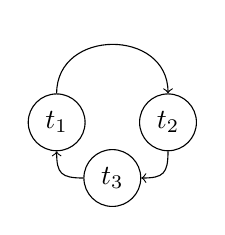
\begin{tikzpicture}[main/.style = {draw, circle}] 
			\node[main] (1) {$t_1$}; 
			\node[main] (3) [below right of=1] {$t_3$}; 
			\node[main] (2) [above right of=3] {$t_2$}; 

			% \draw[->] (1) -- (2);
			\draw[->] (1) to [out=90, in=90, looseness=1.5] (2);
			\draw[->] (2) to [out=270, in=360, looseness=1.5] (3);
			\draw[->] (3) to [out=180, in=270, looseness=1.5] (1);
		\end{tikzpicture} 
	\end{center}

	In the following pages, for metric considerations these terms will be used:

	\begin{itemize}
		\itemsep0sp
		\item \texttt{fps}: number of frames per second.
		\item \texttt{read}: time of execution of the capture thread.
		\item \texttt{for}: time of execution of the elaboration thread. This is what is under discussion in this project.
	\end{itemize}

	\subsection{CPU Implementation}
	The CPU implementation is the easier one and the most basic implementation of the algorithm. It consists on a loop between each byte that compose the two frames (the current one and the previous one) and compute the difference, storing it in a new vector.\\

	The C++ implementation is the following:
	\begin{lstlisting}[style=CStyle]
	int total = 3 * ctx.sampleMat->rows * ctx.sampleMat->cols; // no. bytes
	Mat pvs = pready->pframe->clone();
	pready->h_pos = 0;

	for (int i = 0; i < total; i++) {
		int df = pready->pframe->data[i] - previous.data[i];
		if (df < -LR_THRESHOLDS || df > LR_THRESHOLDS) {
			pready->pframe->data[pready->h_pos] = df;
			pready->h_xs[pready->h_pos] = i;
			pready->h_pos++;
		} else {
			pvs.data[i] -= df;
		}
	}

	previous = pvs;
	\end{lstlisting}

	The code here is pretty simple. For each byte, the difference \texttt{df} is computed. If this difference is greater than a fixed threshold \texttt{LR\_THRESHOLDS} means that it is a valid difference so it can be sent. For all the benchmarks proposed in the following, the value of \texttt{LR\_THRESHOLDS} is fixed to $ 20 $. The result of the reconstructed frame at the client side can be seen at Figure \ref{fig:stream_ok}.\\

	\begin{figure}[H]
		\centering
		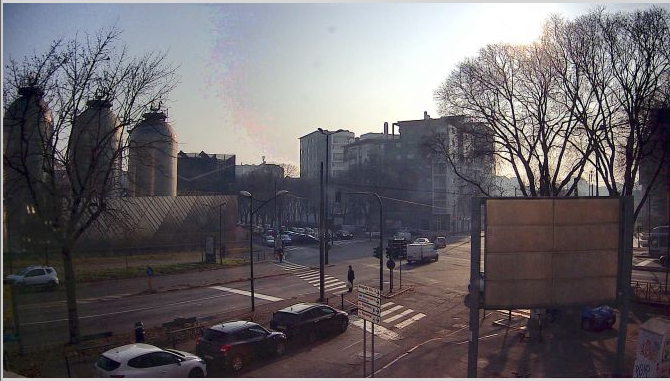
\includegraphics[width=0.7\linewidth]{images/streaming_ok2.png}
		\caption{\textit{The result of the reconstructed frame}}
		\label{fig:stream_ok}
	\end{figure}
	
	The important point here is that if the difference is too low, it can't be simply discarded, so a kind of negative feedback is needed. This is the purpose of the line of code at line 7, where the value of the byte of the current frame (that at the end of the loop will be the previous for the next iteration) is itself minus the value of the difference. This means that at the next iteration, if that value changes again and its difference increases it will take under consideration as a big difference. Without this, there will be a sum of errors in the reconstructed image, leading in a wrong visualization. The result if the error is not considered can be seen at Figure \ref{fig:stream_error}.
	
	\begin{figure}[H]
		\centering
		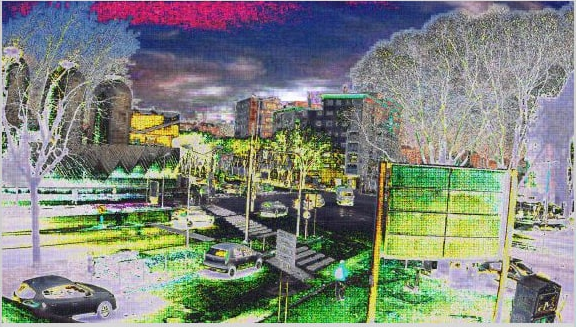
\includegraphics[width=0.7\linewidth]{images/streaming_differror.png}
		\caption{\textit{What happens after a certain time if the error is not take under consideration}}
		\label{fig:stream_error}
	\end{figure}

	The performances here are pretty bad. By means of in-code time measurements, the video streaming is stable at 7 fps with an average \texttt{for} time of 140.0 ms and an average \texttt{read} time of 0.0 ms. This means that here the big bottleneck is due to the elaboration part of the software.

	\begin{figure}[H]
		\centering
		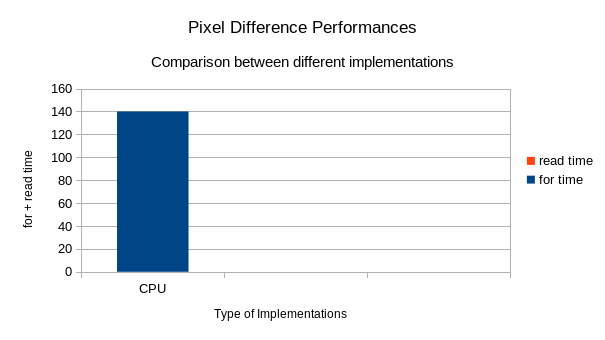
\includegraphics[width=0.8\linewidth]{images/chart1.png}
		\caption{\textit{Pixel Difference Comparison}}
	\end{figure}

	\subsection{GPU Implementation}
	The idea is now to port this in the GPU. The GPU can be seen as an accelerator for the CPU, an accelerator that is capable of a high degree of parallelism by executing a lot of simple threads all in parallel in a SIMD way.\\

	In order to port this in CUDA and execute the computation on the GPU, a series of considerations needs to be done. First of all, it's not said that by executing this in GPU there is a direct improvement in performance. This is due to the fact that there is a big bottleneck between the CPU and the GPU and this is the bus that connects them. A GPU in order to do some work on some data needs to have them in its memory (so the GPU can't access directly the CPU's RAM).\\

	The first thing to do, before defining the kernel (the piece of code that is offloaded to the GPU), is to understand how split the 6220800 bytes among the concurrent threads of the GPU. In the Mat object, the frame is rapresented row-major, means that rows are at consecutive address, as shown in Table \ref{tab:row_major}.

	\begin{table}[H]
		\centering
		\begin{tabular}{ |c:c:c| } 
			\hline
			0 & 1 & 2 \\
			\hdashline
			3 & 4 & 5 \\ 
			\hdashline
			6 & 7 & 8 \\ 
			\hline
		\end{tabular}
		\begin{tabular}{ |c|c|c|c|c|c|c|c|c| } 
			\hline
			0 & 1 & 2 & 3 & 4 & 5 & 6 & 7 & 8 \\
			\hdashline
			0x0 & 0x1 & 0x2 & 0x3 & 0x4 & 0x5 & 0x6 & 0x7 & 0x8 \\
			\hline
		\end{tabular}
	\caption{\textit{Row major rapresentation in memory. On top the value, on bottom the address}}
	\label{tab:row_major}
	\end{table}

	Threads can be organized differently according how they access the memory, and in this case there can be two possible cases of memory access per thread:

	\begin{table}[H]
		\parbox{.45\linewidth}{
			\centering
			\begin{tabular}{l|ccc}
				Thread 0 & 0 & 3 & 6\\
				\hline
				Thread 1 & 1 & 4 & 7\\
				\hline
				Thread 2 & 2 & 5 & 8\\
			\end{tabular}
			\caption{Non consecutive access}
		}
		\hfill
		\parbox{.45\linewidth}{
			\centering
			\begin{tabular}{l|ccc}
				Thread 0 & 0 & 1 & 2\\
				\hline
				Thread 1 & 3 & 4 & 5\\
				\hline
				Thread 2 & 6 & 7 & 8\\
			\end{tabular}
			\caption{Consecutive access}
		}
	\end{table}
	
	So the entire array can be divided into <N> chunks where <N> is the number of threads to launch on the GPU. By organizing the kernels in a way they can access the memory in a consecutive access, the kernel will achieve the so called \textit{memory coalesced access}.\\

	How many threads? For a first implementation, and in order to have a modular implementation of the code (so it can be executed on different GPUs with different capabilities), the following code is adopted:

	\begin{lstlisting}[style=CStyle]
	struct cudaDeviceProp prop;
	cudaGetDeviceProperties(&prop, 0); // retrieves device infos

	int total = 3 * ctx.sampleMat->rows * ctx.sampleMat->cols; // no. bytes
	int nMaxThreads = prop.maxThreadsPerBlock;
	int maxAtTime = total / nMaxThreads;
	\end{lstlisting}

	According to this, each thread will work on $N = \textit{maxAtTime}$ consecutive bytes, dividing the memory into \textit{nMaxThreads} chunks, and overlapping is totally avoided. The GPU used for the experiments allows a maximum of 1024 threads to be executed concurrently.\\

	For what concerns the memory allocation, obviously the CPU address space and the GPU one are two separated things, so a specific allocation on the device side must be done. This can be accomplished thanks to some CUDA's API as follows:

	\begin{lstlisting}[style=CStyle]
	uint8_t *d_current, *d_previous, *d_diff;
	int *d_xs;
	unsigned int *d_pos;

	cudaMalloc((void **)&d_diff, total * sizeof *d_diff);
	cudaMalloc((void **)&d_xs, total * sizeof *d_xs);
	cudaMalloc((void **)&d_current, total * sizeof *d_current);
	cudaMalloc((void **)&d_previous, total * sizeof *d_previous);
	cudaMalloc((void **)&d_pos, sizeof *d_pos);
	\end{lstlisting}


	\subsubsection{Naif version}

	The naif version of the implementation is to port as it is the CPU code into a kernel. From the host side (the CPU) that asks to the device (the GPU) to execute the kernel, there are three kind of operations to be done:

	\begin{enumerate}
		\itemsep0sp
		\item copy the frame into the GPU's memory
		\item launch the kernel
		\item copy back the results from the GPU's memory to the HOST memory
	\end{enumerate}

	In the naif implementation, both the previous and current frames are copied into the GPU's memory. At the end of the execution, the results are copied back. This implies 2 transfers HostToDevice (HtoD) for current and previous and 3 transfers DeviceToHost (DtoH) for h\_xs, h\_diff and h\_pos. A memset on the device side is required too to set the initial value of d\_pos to 0.\\

	The host will therefore execute the following operations:

	\begin{lstlisting}[style=CStyle]
cudaMemset(d_pos, 0, sizeof *d_pos);

// launch
cudaMemcpy(d_previous, previous.data, total, cudaMemcpyHostToDevice);
cudaMemcpy(d_current,pready->pframe->data,total,cudaMemcpyHostToDevice);
kernel<<<1,nMaxThreads>>>(d_current,d_previous,d_diff,maxAtTime,d_pos,d_xs);

// copy back
cudaMemcpy(pready->pframe->data, d_diff, total, cudaMemcpyDeviceToHost);
cudaMemcpy(pready->h_xs, d_xs, total*sizeof *d_xs, cudaMemcpyDeviceToHost);
cudaMemcpy(&pready->h_pos, d_pos, sizeof *d_pos, cudaMemcpyDeviceToHost);

// copy previous
cudaMemcpy(previous.data, d_current, total, cudaMemcpyDeviceToHost);
	\end{lstlisting}

	It's possible to notice a pretty similar structure of the CPU implementation, where the \textit{for loop} is replaced by the kernel. The kernel is launched with a grid dimension of (1, 0, 0) and a block dimension of (\textit{nMaxThreads}, 0, 0), thus only the x dimension is used because the kernel is coded in such a way that the chunk assigned to it is analyzed in a linear way. \\
	
	In order to define the code of the kernel, there are two main problems to be analyzed first:

	\begin{enumerate}
		\itemsep0sp
		\item How does the kernel knows at which address it must work?
		\item How is possible to fill a variable size array in a concurrent environment in CUDA?
	\end{enumerate}

	The first problem is easily solved, it's only a matter of indexes. Each kernel needs to know which chunk of the memory is assigned to it so first of all it computes it's own unique index that will space from 0 to $nMaxThreads - 1$. Once this is defined, the kernel knows that it must work on the i-th chunk but this needs to be translated into the real index to be used to address the memory. Because each size is \textit{maxAtTime} large, means that the the real index that identifies the start of the chunk is $ threadIndex \cdot maxAtTime$.\\

	The second problem is a bit more complicated to solve. In the CPU implementation a variable h\_pos is used in order to indicize the resulting vectors an incremental way and at the end this variable is used to know the length of the result. The problem when this concept is trasposed to the GPU world is that there is a global variable d\_pos that is used by \textit{nMaxThreads} concurrently so there is the need to read and increment this variable in a safe way, so only a kernel at a time can ready and modify it. Luckly, the CUDA framework offers a series of functions that ensures atomic operations between kernels, and in this case the needed one is \texttt{atomicInc(unsigned int *address, unsigned int val)} where \textit{address} is the pointer to the value that needs to be atomic incremented, \textit{val} is the wraparound value, so the max value that the variable can reach before going again to 0, and it returns as result the value atomically incremented.\\

	After solved those problems, a look at the real implementation of the kernel can be given:
	
	\begin{lstlisting}[style=CStyle]
__global__ void kernel(
uint8_t *current, uint8_t *previous, uint8_t *diff, 
int maxSect, unsigned int *pos, int *xs) {
	int x = threadIdx.x + blockDim.x * blockIdx.x;
	unsigned int npos;
	int df;


	int start = x * maxSect;
	int max = start + maxSect;

	#pragma unroll
	for (int i = start; i < max; i++) {

		df = current[i] - previous[i];
		if (df < -LR_THRESHOLDS || df > LR_THRESHOLDS) {
			npos = atomicInc(pos, 6220801);
			diff[npos] = df;
			xs[npos] = i;
		} else {
			current[i] -= df;
		}

	}

}
	\end{lstlisting}

	As can be seen, apart the computation of the start and end index of the computation, the for loop is pretty much the same as the CPU implementation. The only difference is the one concerting the use of the \texttt{atomicInc} function as explained before.\\

	The performances here are slightly better than the CPU implementation. The video streaming is elaborated at around 13 fps with an average \texttt{for} time of 70.0 ms and an average \texttt{read} time of 0.0 ms, and the comparison with the previous case can be seen in Figure \ref{fig:chart2}. 

	\begin{figure}[H]
		\centering
		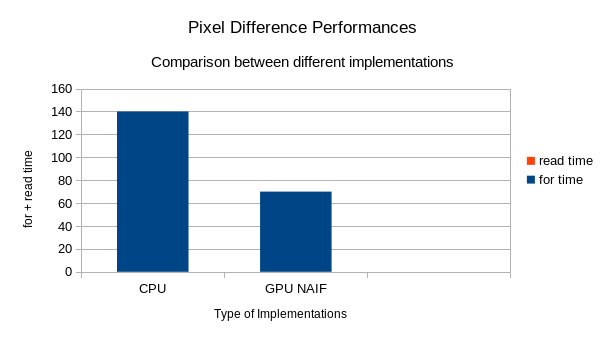
\includegraphics[width=0.8\linewidth]{images/chart2.png}
		\caption{\textit{Pixel Difference Comparison}}
		\label{fig:chart2}
	\end{figure}

	This means that the big bottleneck is still due to the elaboration part of the software. Using the profiler offered by Nvidia \textit{nvprof} executed for 30 seconds, it's possible to get a lot more details about the time required by each GPU operation, and in particular what concerns this project is the transfer time and the kernel execution time. The results are shows in table \ref{tab:nvprof_naif}.

	\begin{table}[H]
		\centering
		\begin{tabular}{||c | c c c||} 
			\hline
			Operation & Avg (ms) & Min (ms) & Max (ms) \\ [0.5ex] 
			\hline\hline
			Kernel & 40.295 & 35.912 & 47.033 \\ 
			\hdashline
			DtoH & 4.2975 & 1.5100 & 52.878 \\
			\hdashline
			HtoD & 3.3280 & 2.4544 & 25.808 \\
			\hdashline
			Memset & 0.0008 & 0.0007 & 0.0017 \\
			\hline
		\end{tabular}
		\caption{Profiling results}
		\label{tab:nvprof_naif}
	\end{table}

	\subsubsection{Asynchronous APIs and removal of useless operations}

	In the previous implementation, a big portion of the execution time is covered by the kernel execution but the two data transfers are not negligible. The total average time is about 46 ms means that the \textit{for} time is for the 60\% due to the GPU computation and the remaining part is related to host taks.\\

	CUDA offsers a variant of the APIs that are asynchronous with respect to the device execution. This means that when one of these APIs is called, the operation starts on the device side but the control returns immediately to the host despite the end of the operation on the GPU.\\

	This means that is possible to give to the device a series of operations to execute and meanwhile the host can work on its own operations. In this specific case the host doesn't have any task to complete so a function \texttt{cudaDeviceSynchronize()} is used to wait for the device to complete its operations. Howewer this solution is slightly more efficient because is possible to assign to the GPU all the jobs in a consecutive way then waiting instead of assign a job at a time.

	\begin{lstlisting}[style=CStyle]
cudaMemsetAsync(d_pos, 0, sizeof *d_pos);

cudaMemcpyAsync(d_previous, previous.data, total, cudaMemcpyHostToDevice);
cudaMemcpyAsync(d_current,pready->pframe->data,total,cudaMemcpyHostToDev);
kernel<<<1,nMaxThreads>>>(d_current,d_previous,d_diff,maxAtTime,d_pos,d_xs);

cudaMemcpyAsync(pready->pframe->data, d_diff, total,cudaMemcpyDeviceToHost);
cudaMemcpyAsync(pready->h_xs,d_xs,total*sizeof *d_xs,cudaMemcpyDevToHost);
cudaMemcpyAsync(&pready->h_pos,d_pos,sizeof *d_pos, cudaMemcpyDeviceToHost);

cudaMemcpyAsync(previous.data, d_current, total, cudaMemcpyDeviceToHost);
cudaDeviceSynchronize();
	\end{lstlisting}


	Another optimization that can be done is to remove a particular useless copy both HtoD and DtoH, and that is the one regarding the previous frame. In fact, after the first launch of the kernel, the previous frame is already stored in the GPU's memory so it's avoidable the back copy to the host and gain to the device. What can be done is to implement a simple pointer swap, in fact after the first execution the current frame will become the previous frame at the next round. So there is a pool of two pointers that alternatively works one as the current and the other one as the previous.\\

	The host code becomes like this:

	\begin{lstlisting}[style=CStyle]
// current-previous swap
uint8_t *d_prev = d_current;
d_current = d_previous;
d_previous = d_current;

cudaMemsetAsync(d_pos, 0, sizeof *d_pos);

// Copy in the current pointer and run 
cudaMemcpyAsync(d_current,pready->pframe->data,total,cudaMemcpyHostToDeve);
kernel<<<1,nMaxThreads>>>(d_current,d_previous,d_diff,maxAtTime,d_pos,d_xs);

cudaMemcpyAsync(pready->pframe->data,d_diff,total,cudaMemcpyDeviceToHost);
cudaMemcpyAsync(pready->h_xs,d_xs,total*sizeof *d_xs,cudaMemcpyDevToHost);
cudaMemcpyAsync(&pready->h_pos,d_pos,sizeof *d_pos,cudaMemcpyDeviceToHost);

cudaDeviceSynchronize();
	\end{lstlisting}

	Another optimization in terms of copies regards the download of the two arrays forming the result. In fact, instead of copying all the \textit{total} bytes is smarter to cpy only \textit{d\_pos} bytes, the ones that are really useful.\\

	So the first download copy regards \textit{d\_pos}, then a \texttt{cudaDeviceSynchronize()} is executed in order to wait for the complete of all the previous operation and getting a valid \textit{d\_pos}, then the remaining data are copied. \\
	
	The host code becomes:

	\begin{lstlisting}[style=CStyle]
// current-previous swap
uint8_t *d_prev = d_current;
d_current = d_previous;
d_previous = d_current;

cudaMemsetAsync(d_pos, 0, sizeof *d_pos);

// Copy in the current pointer and run 
cudaMemcpyAsync(d_current,pready->pframe->data,total,cudaMemcpyHostToDeve);
kernel<<<1,nMaxThreads>>>(d_current,d_previous,d_diff,maxAtTime,d_pos,d_xs);

cudaMemcpyAsync(&pready->h_pos,d_pos,sizeof *d_pos,cudaMemcpyDeviceToHost);
cudaDeviceSynchronize();

cudaMemcpyAsync(pready->pframe->data,pready->h_pos,total,cudaMemcpyDToHt);
cudaMemcpyAsync(pready->h_xs,d_xs,pready->h_pos*sizeof *d_xs,cdMemcpyDToH);


cudaDeviceSynchronize();
	\end{lstlisting}

	Last but not least, the \textit{cudaMemsetAsync} at line 6 can be removed completely. In fact, it's possible to move the initial reset of the \textit{d\_pos} counter by doing it at the beginning of the kernel and it's easily done even in a concurrent environment by letting only one kernel to perform the reset. This can be achieved by putting a condition on the kernel index. In this case it will be done by the first kernel. In order to have all the kernel executing more or less in parallel the same instructions, after the reset of the counter, a \texttt{\_\_syncthreads()} is executed that assures that all threads are synchred untill that point. \\

	Thus, the kernel code becomes:

	\begin{lstlisting}[style=CStyle]
__global__ void kernel(
uint8_t *current, uint8_t *previous, uint8_t *diff, 
int maxSect, unsigned int *pos, int *xs) {
	int x = threadIdx.x + blockDim.x * blockIdx.x;
	unsigned int npos;
	int df;

	// counter reset done by thread with index = 0
	if (!x) *pos = 0;
	__syncthreads();


	int start = x * maxSect;
	int max = start + maxSect;

	#pragma unroll
	for (int i = start; i < max; i++) {

		df = current[i] - previous[i];
		if (df < -LR_THRESHOLDS || df > LR_THRESHOLDS) {
			npos = atomicInc(pos, 6220801);
			diff[npos] = df;
			xs[npos] = i;
		} else {
			current[i] -= df;
		}

	}

}
	\end{lstlisting}

	All these optimizations let achieve a big result in performance terms. The video streaming is elaborated at around 20 fps with an average \texttt{for} time of 55.0 ms and an average \texttt{read} time of 0.0 ms, and the comparison with the previous case can be seen in Figure \ref{fig:chart3}. 

	\begin{figure}[H]
		\centering
		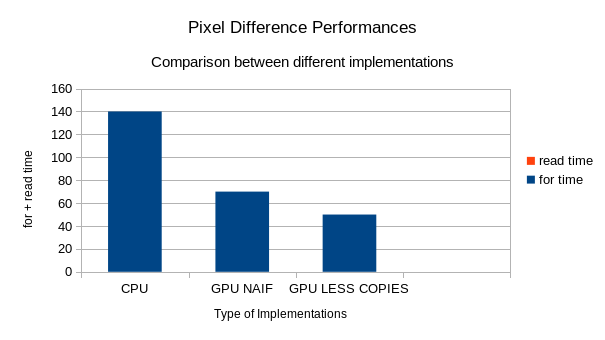
\includegraphics[width=0.8\linewidth]{images/chart3.png}
		\caption{\textit{Pixel Difference Comparison}}
		\label{fig:chart3}
	\end{figure}

	The results of the \textit{nvprof} profiler are shown in Table \ref{tab:nvprof_naif2} and is noticeable the big improvement in terms of performances for what concerns the DtoH transfer. The HtoD transfer remains more or less the same but it's executed only one time instead of two as the naif implementation.

	\begin{table}[H]
		\centering
		\begin{tabular}{||c | c c c||} 
			\hline
			Operation & Avg (ms) & Min (ms) & Max (ms) \\ [0.5ex] 
			\hline\hline
			Kernel & 41.426 & 37.278 & 46.423 \\ 
			\hdashline
			DtoH & 0.0227 & 0.0009 & 9.2925 \\
			\hdashline
			HtoD & 3.7813 & 2.1733 & 14.188 \\
			\hline
		\end{tabular}
		\caption{Profiling results}
		\label{tab:nvprof_naif2}
	\end{table}

	\subsubsection{Pinned or page-locked memory}

	Untill now a good bottleneck has been removed and it is the transfer from the Device to the Host. What about the Host to Device transfer? In order to solve this issue an understanding on how memory is managed by the CPU and how the GPU transfers data from the CPU's managed memory and the GPU.\\

	What a modern operating system does is to manage the physical memory through the concept of pages and thus the virtual memory. The address space of the virtual memory is different from the physical one, thus a translation is needed. In order to let the hardware translate from a space to another, a special hardware called translation lookaside buffer (TLB) is used. It's a memory cache that is used to reduce the time taken to access a user memory location and it's part of the chip's memory-management unit (MMU) needed in fact by all the modern operating systems. The TLB stores the recent translations of virtual memory to physical memory and can be called an address-translation cache.\\

	When a CUDA's memcpy is invoked, the DMA starts transfering data but as soon as the translation is not anymore stored in the cache, the operating system has to solve this situation by loading a new page. Thus this is not really a asynchronous operation and it's highly cpu-dependent. Thus the velocity of the copy is based on the speed of the CPU and in edge devices where the CPU is not so performant as a desktop CPU the overhead of this mechanism can't be neglected.\\
	
	The solution is to allocate a piece of memory that is pinned or \textit{page locked}. Executing an allocation like this is like telling the operating system virtual memory manager that the memory pages must stay in physical ram so that they can be directly accessed by the GPU across the PCI-express bus. And it's a lot faster thanks to the DMA: when the memory is page locked, the GPU DMA engine can directly run the transfer without requiring the host CPU, which reduces overall latency and decreases transfer times.\\

	CUDA offers an API to do this, called \texttt{cudaMallocHost()} that works similar to \texttt{cudaMalloc()} but allocates a page-locked memory on the host side. It's required for arrays like \texttt{h\_xs} and \texttt{pready->pframe->data}. If it's pretty easy to be done for \texttt{h\_xs} that is an array directly managed by the code, how is possible to do that for the pframe's data that is something managed by OpenCV? As said at the beginning, the \textit{Mat} object offers a good option, the one to select an external pointer as data array.\\

	\begin{lstlisting}[style=CStyle]
uint8_t *h_frame;
cudaMallocHost((void **)&h_frame, total * sizeof *h_frame);
cudaMallocHost((void **)&pready->h_xs, total * sizeof *pready->h_xs);

// init of Mat object with page-locked h_frame ptr
pready->pframe = new Mat(ctx.sampleMat->rows,ctx.sampleMat->cols,
		ctx.sampleMat->type(), h_frame); 
	\end{lstlisting}

	Without touching anything else, this optimization is able to achieve a good result. The video streaming is elaborated at around 22 fps with an average \texttt{for} time of 43.0 ms and an average \texttt{read} time of 0.0 ms, and the comparison with the previous case can be seen in Figure \ref{fig:chart4}. 

	\begin{figure}[H]
		\centering
		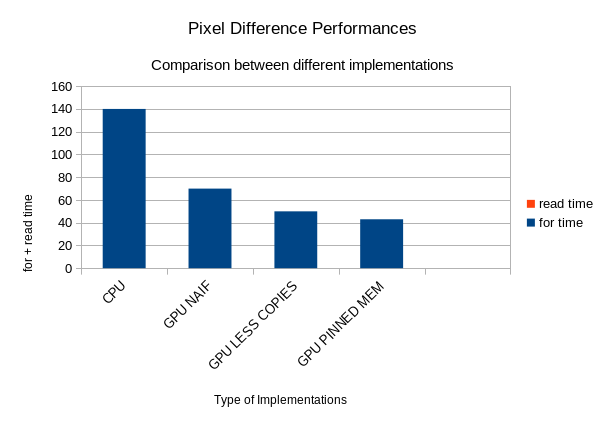
\includegraphics[width=0.8\linewidth]{images/chart4.png}
		\caption{\textit{Pixel Difference Comparison}}
		\label{fig:chart4}
	\end{figure}

	The results of the \textit{nvprof} profiler are shown in Table \ref{tab:nvprof_naif3} and is noticeable the big improvement in terms of performances for what concerns the HtoD transfer. In fact, it's about 1/4 the original one.

	\begin{table}[H]
		\centering
		\begin{tabular}{||c | c c c||} 
			\hline
			Operation & Avg (ms) & Min (ms) & Max (ms) \\ [0.5ex] 
			\hline\hline
			Kernel & 43.386 & 38.093 & 49.607 \\ 
			\hdashline
			DtoH & 0.0102 & 0.0008 & 1.0466 \\
			\hdashline
			HtoD & 0.6740 & 0.6096 & 2.2818 \\
			\hline
		\end{tabular}
		\caption{Profiling results}
		\label{tab:nvprof_naif3}
	\end{table}

	\subsubsection{Kernel global memory access: the cherry on the cake}
	\label{sec:cherry}

	What remains now to further optimize is the kernel execution time. Doing a bunch of analysis, with a maximum number of threads of 1024 each kernel execute a \textit{for loop} that lasts 6075 iterations. Each iteration access in memory three times in the most of the cases (supposing $ N_{pixelChanged} \ll N_{pixelNotChanged} $) and accesses in global memory are a real bit bottleneck for CUDA's kernel because usually the Global memory access time is $400 \sim 600$ cycles. Obviously, each byte needs to be esaminated so it's not possible to randomly cut accesses in memory. How this can be optimized?\\

	The answer to this question is very simple but at the same time it's brilliant: by increase the size of each read or write in memory. By applying this concept, both the memory accesses and the loop iterations are reduced, so it's an optimization in both ways.\\

	The first think to do is to rewrite the kernel in order to support this. The idea is to load into some GPU's registers some bytes regarding a portion of the current and previous frame under consideration by the for loop of a kernel. Then there is always need of a byte-wise substraction and comparison so a inner for loop will access byte-wise the word loaded into the register(s) and will do its computations.\\

	The multi-byte memory access is done using the dynamic pointer cast feature, casting the vector pointers to the data type aimed, Therefore the new kernel implementation, using the most common data type that is the \texttt{int} one, is:

	\begin{lstlisting}[style=CStyle]
typedef int chunk_t;

__global__ void kernel2(
uint8_t *current, uint8_t *previous, uint8_t *diff, 
int maxSect, unsigned int *pos, int *xs) {
    int x = threadIdx.x + blockDim.x * blockIdx.x;
    unsigned int npos;
    int df;
    chunk_t cc, pc; // registers storing current copy, previous copy

    if (!x) *pos = 0;
    __syncthreads();

    int start = x * maxSect;
    int max = start + maxSect;

    #pragma unroll
    for (int i = start; i < max; i++) {

        cc = ((chunk_t *)current)[i];
        pc = ((chunk_t *)previous)[i];

        #pragma unroll
        for (int j = 0; j < sizeof cc; j++) {
            df = ((uint8_t *)&cc)[j] - ((uint8_t *)&pc)[j];

            if (df < -LR_THRESHOLDS || df > LR_THRESHOLDS) {
                npos = atomicInc(pos, 6220801);
                diff[npos] = df;
                xs[npos] = (i*sizeof cc) + j;
            } else {
                current[(i*sizeof cc) + j] -= df;
            }

        }

    }

}
	\end{lstlisting}

	The host code changes a little bit because maxAtTime now needs to be divided by the size of the \texttt{chunk\_t} type. Because it's highly probable that the division results in a non integer value, it must be rounded to the nearest greater integer. \\
	
	This means that by rounding up, each thread will overlap with the next thread of a few bytes. Actually it's not a problem because the probability that while the thread \textit{i} writes at the very last bytes of its chunk the thread \textit{i+1} writes at the very beginning of its chunk is very low because each thread is executed in parallel. The only thing that happens is that the computations on a certain amount of bytes is done two times but each time it's done on the same inputs and the result is always the same. In a low probability case where two writes at the same time happens, as discussed, the overhead in managing the concurrent write is lower than the one of adding instructions to check if the thread is writing outside its chunk (about 1 ms of difference in execution time).\\

	\begin{lstlisting}[style=CStyle]
int max4 = ceil(1.0 * maxAtTime / sizeof(chunk_t));

// CUDA APIs call
// ...
kernel2<<<1,nMaxThreads>>>(d_current,d_previous, d_diff, max4, d_pos, d_xs);
// ...
\end{lstlisting}

	The only problem to manage by choosing the path of not adding any check inside the kernel is that the last kernel can write outside the memory. In order to avoid wrong memory accesses, the allocaiton of the memory on the GPU is done by considering this margin. In fact, a thread will write at most \texttt{sizeof(chunk\_t)} bytes outside the memory, so each memory allocation is done by allocating an additional amount of bytes equal to \texttt{sizeof(chunk\_t)} bytes:

	\begin{lstlisting}[style=CStyle]
uint8_t *h_frame;
cudaMallocHost((void **)&h_frame, total * sizeof*h_frame + sizeof(chunk_t));
cudaMallocHost((void **)&pready->h_xs,tot*sizeof*prdy->hxs+sizeof(chunk_t));

// init of Mat object with page-locked h_frame ptr
pready->pframe = new Mat(ctx.sampleMat->rows,ctx.sampleMat->cols,
		ctx.sampleMat->type(), h_frame); 
	\end{lstlisting}

	The results of the \textit{nvprof} profiler are shown in Table \ref{tab:nvprof_naif4} and is noticeable the big improvement in terms of performances for what concerns the Kernel execution time. In fact, it's almost the 50\% of the previous implementation. The average fps are 21, with a \textit{for} time of 26.0 ms and a \textit{read} time of 30 ms.

	\begin{table}[H]
		\centering
		\begin{tabular}{||c | c c c||} 
			\hline
			Operation & Avg (ms) & Min (ms) & Max (ms) \\ [0.5ex] 
			\hline\hline
			Kernel & 23.700 & 21.590 & 24.671 \\ 
			\hdashline
			DtoH & 0.0079 & 0.0008 & 1.0009 \\
			\hdashline
			HtoD & 0.6483 & 0.6074 & 2.5641 \\
			\hline
		\end{tabular}
		\caption{Profiling results}
		\label{tab:nvprof_naif4}
	\end{table}

	A further optimization can be done by looking at the new kernel implementation and noticing that only 2/3 of the memory accesses are optimized. The feedback write in fact is still done at each byte, and it can be easily optimized by modifying the \texttt{cc} register variable in the inner loop (byte wise) and save back the result in the global memory at the end of the inner loop only if needed (so if the \texttt{cc} variable has been modified).\\
	
	The implementation is the following:

	\begin{lstlisting}[style=CStyle]
typedef int chunk_t;

__global__ void kernel2(
uint8_t *current, uint8_t *previous, uint8_t *diff, 
int maxSect, unsigned int *pos, int *xs) {
    int x = threadIdx.x + blockDim.x * blockIdx.x;
    unsigned int npos;
    int df;
    chunk_t cc, pc; // registers storing current copy, previous copy
    bool currUpdateRequired = false;

    if (!x) *pos = 0;
    __syncthreads();

    int start = x * maxSect;
    int max = start + maxSect;

    #pragma unroll
    for (int i = start; i < max; i++) {

        cc = ((chunk_t *)current)[i];
        pc = ((chunk_t *)previous)[i];

        #pragma unroll
        for (int j = 0; j < sizeof cc; j++) {
            df = ((uint8_t *)&cc)[j] - ((uint8_t *)&pc)[j];

            if (df < -LR_THRESHOLDS || df > LR_THRESHOLDS) {
                npos = atomicInc(pos, 6220801);
                diff[npos] = df;
                xs[npos] = (i*sizeof cc) + j;
            } else {
                ((uint8_t *)&cc)[j] -= df;
                currUpdateRequired = true;
            }

        }

        // storing in global memory only if needed
        if (currUpdateRequired) {
        	((chunk_t *)current)[i] = cc;
        	currUpdateRequired = false;
        }
    }

}
	\end{lstlisting}

	The results of the \textit{nvprof} profiler are shown in Table \ref{tab:nvprof_naif5} and is noticeable another big improvement, reducing the kernel time by another 50\%. The average fps are 24, with a \textit{for} time of 11.5 ms and a \textit{read} time of 40 ms. The overall comparison is shown in Figure \ref{fig:chart5}.

	\begin{table}[H]
		\centering
		\begin{tabular}{||c | c c c||} 
			\hline
			Operation & Avg (ms) & Min (ms) & Max (ms) \\ [0.5ex] 
			\hline\hline
			Kernel & 9.7944 & 8.7887 & 17.906 \\ 
			\hdashline
			DtoH & 0.0080 & 0.0008 & 1.2807 \\
			\hdashline
			HtoD & 0.6443 & 0.5969 & 2.9633 \\
			\hline
		\end{tabular}
		\caption{Profiling results}
		\label{tab:nvprof_naif5}
	\end{table}

	\begin{figure}[H]
		\centering
		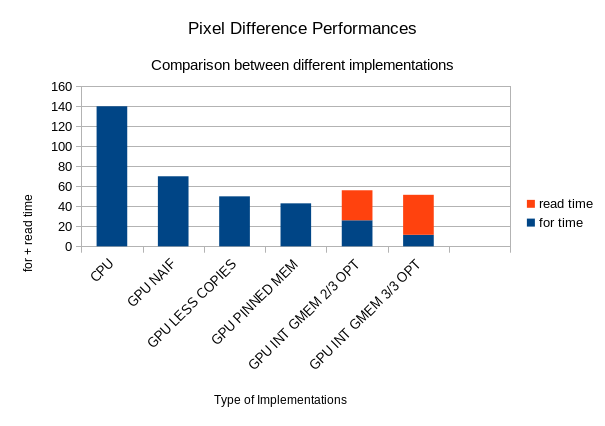
\includegraphics[width=0.8\linewidth]{images/chart5.png}
		\caption{\textit{Pixel Difference Comparison}}
		\label{fig:chart5}
	\end{figure}

	The overall situation can be optimized even more. CUDA offers the possibility to perform vectorized memory accesses by using \textit{vectorized data types}. What are them and why they are so important?\\

	First of all, these special data types are of different types depending on their reference type. For example there is \texttt{int2}, \texttt{float3}, \texttt{ulong2} and so on. Looking at the public header files they are defined as follow (taking \texttt{int4} as an example):

	\begin{lstlisting}[style=CStyle]
struct __device_builtin__ __builtin_align__(16) int4 {
    int x, y, z, w;
};

typedef __device_builtin__ struct int4 int4;\end{lstlisting}

	Thanks to the fact they they are \texttt{\_\_device\_builtin\_\_}, they are identified by the CUDA compiler that will optimize the generated instructions by reducing them and using special \textit{vectorized instructions} capable of a larger transaction in the memory. So thanks to these instructions is possible to load big chunks of data at a time with less instructions. Please note that a common struct with 16 int variables as members will not perform well as expected because int4 is a builtin type so recognized by the compiler and vectorized instructions will be used by activating some internal magic in the compiler itself.\\

	The usage of these vectorized instructions is easily seen at the assembly level. The kernel seen before with a classical \texttt{int} data type is translated into these instructions:

	\begin{lstlisting}[style=CStyle]
/*00c8*/ MOV R3, R5;
/*00d0*/ LD.E R18, [R10];
/*00d8*/ LD.E R14, [R2]; 
/*00e0*/ SSY 0x240;      \end{lstlisting}

	The two LD.E instructions are the one corresponding to the two reads from the global memory into the \texttt{cc} and \texttt{pc}. The LD.E is a scalar instruction that will load a word from memory. Using instead \texttt{int4} builtin type, the disassembly code will be:

	\begin{lstlisting}[style=CStyle]
/*00c8*/ MOV R3, R17;        
/*00d0*/ MOV R12, R0;        
/*00d8*/ LD.E.128 R4, [R2];  
/*00e0*/ SSY 0x360;          
/*00e8*/ LD.E.128 R8, [R12]; \end{lstlisting}

	Here, the two LD.E.128 are vectorized instructions. By using the vectorized load and store instructions LD.E.\{64,128\} (and the counter part ST.E.\{64,128\}) operations like load and store data can be done in 64- or 128-bit widths. Using vectorized loads reduces the total number of instructions, reduces latency, and improves bandwidth utilization.\\

	% A small tip. As said these kind of instructions are \textit{vectorized}. They are called in this way because works on a kind of vector and this can be seen in two ways. The first one is looking at the definition of the vectorized type: the \texttt{int4} for example is a struct made of four \texttt{int} so it's a vector of in this sense. Looking at the assembly code instead is possible to see how the two 

	At this point, the \textit{nvprof} profiler is run and the results are shown in Table \ref{tab:nvprof_naif6} and is noticeable a really big improvement in the computation, reducing the kernel time by another 60\%. The average fps are 26, with a \textit{for} time of 4.7 ms and a \textit{read} time of 37 ms. 

	\begin{table}[H]
		\centering
		\begin{tabular}{||c | c c c||} 
			\hline
			Operation & Avg (ms) & Min (ms) & Max (ms) \\ [0.5ex] 
			\hline\hline
			Kernel & 3.4197 & 2.9266 & 9.0223 \\ 
			\hdashline
			DtoH & 0.0061 & 0.0008 & 1.1601 \\
			\hdashline
			HtoD & 0.6387 & 0.5957 & 2.5595 \\
			\hline
		\end{tabular}
		\caption{Profiling results}
		\label{tab:nvprof_naif6}
	\end{table}

	Even if the 128 bit width is the maximum width support, it's possible to optimize the resulting code even more at the instruction level by using a larger builtin types like \texttt{long4}. As can be intuitable, it will be translated into 2 instructions. This helps introducing a slightly optimization by reducing the memory access frequency, achieving an average reduction of 0.4 ms in the kernel execution time.\\

	The resulting assembly code is the following one, where is possible to notice two loads at a time with the first one loading at offset \texttt{0x0} as the normal one and the second one loads at offset \texttt{0x10} that is 128 bit far from the first load, thus with two instructions a total of 256 bit or 32 byte are loaded, that is the size of a \texttt{long4} data type.
	
	\begin{lstlisting}[style=CStyle]
/*00c8*/ MOV R3, R13;
/*00d0*/ LD.E.128 R8, [R20];
/*00d8*/ LD.E.128 R4, [R20+0x10];
/*00e0*/ SSY 0x1e0;
/*00e8*/ LD.E.128 R12, [R2];
/*00f0*/ LD.E.128 R16, [R2+0x10]; \end{lstlisting}
	
	The overall comparison is shown in Figure \ref{fig:chart6}.

	\begin{figure}[H]
		\centering
		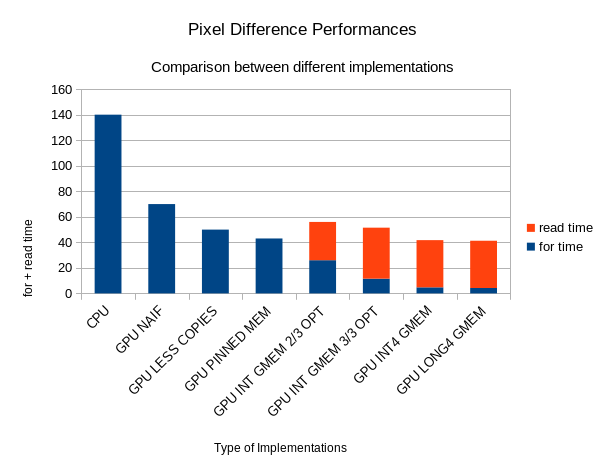
\includegraphics[width=0.9\linewidth]{images/chart6.png}
		\caption{\textit{Pixel Difference Comparison}}
		\label{fig:chart6}
	\end{figure}

	In other words, by using \textit{vectorized instructions} the performance improvement comes from efficiency gains, in two ways:

	\begin{enumerate}
		\item At the instruction level, a multi-word vector load or store only requires a single instruction to be issued, so the bytes per instruction ratio is higher and total instruction latency for a particular memory transaction is lower.
		\item At the memory controller level, a vector sized transaction request from a warp results in a larger net memory throughput per transaction, so the bytes per transaction ratio is higher. Fewer transaction requests reduces memory controller contention and can produce higher overall memory bandwidth utilization.
	\end{enumerate}

	\subsubsection{Using of shared memory for frequent accesses: is it avoidable?}

	Unfortunately, the algorithm and the relative CUDA kernel implementation doesn't show up any pattern of frequent access of the same data over the time, this is because the kernel works everytime on two frames and they differs continuously with respect to the previous kernel execution. \\

	Looking at the last and very optimal kernel implementation, the only frequent global memory access where the same data is read and maybe updated is the one regarding the count of pixel changed or \texttt{h\_pos}. This means that it's reasonable to think to execute the increment operation \texttt{atomicInc()} in the shared memory and then tranfer the final result in the global memory in order to have only one access in global memory per thread with respect to the pixel count variable.\\

	A possible implementation can be the following one:
	\begin{lstlisting}[style=CStyle]
typedef long4 chunk_t;

__global__ void kernel2(
uint8_t *current, uint8_t *previous, uint8_t *diff, 
int maxSect, unsigned int *pos, int *xs) {
    int x = threadIdx.x + blockDim.x * blockIdx.x;
    unsigned int npos;
    int df;
    chunk_t cc, pc; // registers storing current copy, previous copy
    __shared__ unsigned int s_pos[1];

    if (!x) *s_pos = 0;
    __syncthreads();

    int start = x * maxSect;
    int max = start + maxSect;

    #pragma unroll
    for (int i = start; i < max; i++) {

        cc = ((chunk_t *)current)[i];
        pc = ((chunk_t *)previous)[i];

        #pragma unroll
        for (int j = 0; j < sizeof cc; j++) {
            df = ((uint8_t *)&cc)[j] - ((uint8_t *)&pc)[j];

            if (df < -LR_THRESHOLDS || df > LR_THRESHOLDS) {
                npos = atomicInc(s_pos, 6220801);
                diff[npos] = df;
                xs[npos] = (i*sizeof cc) + j;
            } else {
                current[(i*sizeof cc) + j] -= df;
            }

        }

    }

    __syncthreads();
    if (!x) *pos = *s_pos;

}
	\end{lstlisting}

	Notice the use of the function \texttt{\_\_syncthreads()} at the end. It is used to wait for all threads to finish in order to be sure that all the \texttt{atomicInc()} instructions have been executed. After this operation, the global memory variable \texttt{pos} is updated with the value stored in the shared memory variable \texttt{s\_pos} by the first thread, the one with $ id = 0 $.\\

	Unfortunately the result is something unexpected: the performance are exactly the same or a bit worse than the previous implementation. This is mainly for two reasons:

	\begin{enumerate}
		\item As explained in section \ref{sec:cherry}, the part of code where the \texttt{atomicInc()} function is executed is the one with a lower execution frequency because it's supposed that between a frame and another only a bunch of pixels changes so it's not worth trying to improve it that requires adding other instructions (for example the one at the end of the kernel of synchronization) that only adds overhead.
		\item Atomic instructions are very particular: they rely on the bottom hardware for executing memory operations in an atomic way.
	\end{enumerate}

	About the last point, atomic memory operations are very important in parallel programming, allowing concurrent threads to correctly perform read-modify-write operations on shared data. About the importance of how these kind of operations are implemented in CUDA architectures, as an example the Kepler architecture can be analyzed. It significantly increased the throughput of atomic operations to global memory compared to the earlier Fermi architecture; however, both Fermi and Kepler implemented shared memory atomics using an expensive lock/update/unlock pattern. So they were implemented totally in software.\\

	However, Maxwell architecture (the GPU on the \textit{Jetson Nano} used for this projct is based on this architecture) improved this by implementing native hardware support for shared memory atomic operations for 32-bit integers, and native shared memory 32-bit and 64-bit compare-and-swap (CAS), which can be used to implement other atomic functions with reduced overhead (compared to the Fermi and Kepler methods which were implemented in software).\\

	So atomic operations have not been an easy thing. They are very performant for working in the global memory and \textit{only recently} they have been optimized to work in the shared memory with near the same performance compared to the global memory.

	% TODO:
	% \begin{itemize}
	% 	\item Copying both previous and current everytime and no fixed page host allocation
	% 	\item Copying only the current and the previous is a swap pointer, still no fixed page host allocation
	% 	\item Page host allocation
	% 	\item Copy of all d\_diff and d\_xs
	% 	\item Copy first d\_pos then a portion of d\_diff and d\_xs according to d\_pos
	% 	\item Access int-by-int
	% 	\item AtomicInc in global memory and in shared memory, there are differences?
	% 	\item Why 512 kernels is best instead of 1024?
	% \end{itemize}

\section{Image Text Overlay}

	Another part of the project under discussion is the ability to add a text overlay over an image. In this particular implementation, it supports ASCII characters over a single line of the image. In order to be sent over internet, it's executed before applying the algorithm for sent the frame over a socket, according to Chapter \ref{sec:streaming}.\\

	The final result can be seen in Figure \ref{fig:demo_chars}:

	\begin{figure}[H]
		\centering
		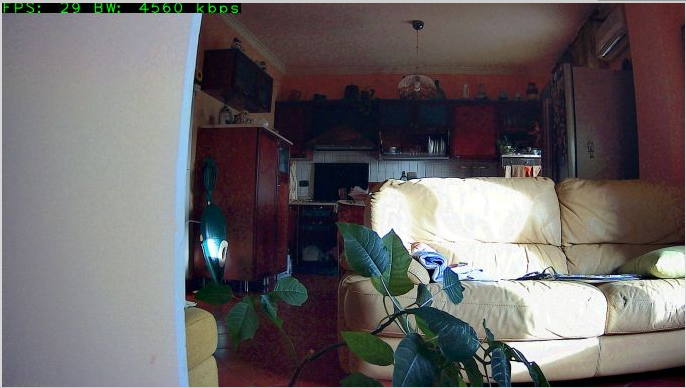
\includegraphics[width=0.9\linewidth]{images/chars_ok.png}
		\caption{\textit{Text Overlay}}
		\label{fig:demo_chars}
	\end{figure}

	The basic idea behind the implementation is the ability to generate a frame (made of RGB pixels) of an ASCII character, dynamically and based on an available font. Everything starts from the specification of the supported alphabet. In fact, not all ASCII characters are supported but only a limited set, specified during the compilation time, in order to have an efficient code in terms of memory occupied and execution time without wasting useful resources (both on the host side and on the device side) for characters that are never used.\\

	After defining the alphabet, at the beginning of the program, it's possible to translate each character into a set of pixels composing it. This is done thanks to a series of OpenCV's function like \texttt{cv::getTextSize} that is able to rietrieve the frame dimensions (width and height) of a character and \texttt{cv::putText} that is able to put a text (or a character in this case) over a frame.\\

	First thing that is done is to retrieve the dimension of a character. This is done only for a single character and it is supposed that all the other characters in the alphabet have the same size.\\

	Than, an array storing all the frames one after another is created with a size that is equal to $ n_{chars} \cdot Area_{char} $. A loop on the alphabet will fill this array with all the character' frames. The code to implement this is the following:

	\begin{lstlisting}[style=CStyle]
#define CHARS_STR "0123456789BFPSWbkps :"

auto txtsz = cv::getTextSize("A", cv::FONT_HERSHEY_PLAIN, 3, 2, 0);
int fullArea = 3 * txtsz.area();
	
uint8_t *charsPx = new uint8_t[(sizeof(CHARS_STR) - 1) * fullArea];
memset(charsPx, 0x0, (sizeof(CHARS_STR) - 1) * fullArea);
for (int i = 0; i < (sizeof(CHARS_STR) - 1); i++) {
	Mat pxBaseMat(txtsz.height, txtsz.width, base.type(), charsPx+i*fullArea);
	cv::putText(pxBaseMat, std::string(CHARS_STR).substr(i, 1),
			cv::Point(0, txtsz.height+1), cv::FONT_HERSHEY_PLAIN, 3,
			cv::Scalar(0, 255, 0), 2, cv::LINE_AA);
}\end{lstlisting}

When the array is finally full filled, it's ready to be copied onto the GPU memory. This operation is done only at the beginning, so it's ininfluent from the point of view of the performances:

	\begin{lstlisting}[style=CStyle]
uint8_t *d_charsPx;
int totcpy = fullArea * sizeof *d_charsPx * (sizeof(CHARS_STR) - 1);
cudaMalloc((void **)&d_charsPx, totcpy * sizeof *d_charsPx);
cudaMemcpy(d_charsPx,charsPx,totcpy*sizeof*d_charsPx,cudaMemcpyHostToDev);
\end{lstlisting}

\subsection{GPU Implementation}
After the initialization phase, is now time to give a look at how each character frame is placed onto the image. It's a replacement of the pixels of the frame under analysis with the one of the corresponding character.\\

The first thing to do is to decide how many kernel to launch and how many pixel each kernel needs to manage. By deciding to assign to each kernel a certain number of pixel in a row-major fashion, and by considering the fact that the frame size of each character is fixed but can change if the font is changed, a portion of the code is used to decide in a dynamic way the two values: number of kernels and pixels for each kernel. It's decided by dividing the total number of bytes of a character frame by the number of frame and if it's a multiple of the size of \texttt{chunk\_t} type that for a first analysis will be a \texttt{uint8\_t}, then the number of threads found is the right one. The code is the following:

	\begin{lstlisting}[style=CStyle]
typedef uint8_t chunk_t;

int nThreadsToUse = nMaxThreads;
int eachThreadDoes = 1;
for (int i = nMaxThreads; i > 0; i--) {
	float frac = fullArea / (i * 1.0);
	int frac_int = fullArea / i;
	if ((int)ceil(frac) == frac_int && frac_int % sizeof(chunk_t) == 0) {
		nThreadsToUse = i;
		eachThreadDoes = frac_int / sizeof(chunk_t);
		break;
	}
}
\end{lstlisting}

\subsubsection{Naif version}

After the setup time, its the turn of the computation step. This is the core, where each character of the string to print is analyzed before applying the streaming algorithm. This is done on the host side and not on the device side in order to avoid the copy HtoD of the string.\\

The advantage is given by the usage of async operations, so while the frame is copied on the GPU, the host scans each character and a new kernel is fired in an async way in order to print each character one after the another.

	\begin{lstlisting}[style=CStyle]
// Copy in the current pointer and run 
cudaMemcpyAsync(d_current,pready->pframe->data,total,cudaMemcpyHostToDev);

for (int offset = 0, j = 0; j < text.length(); j++, offset+=txtsz.width*3) {
	int idx;
	for (int i = 0; i < (sizeof(CHARS_STR) - 1); i++) {
		if (CHARS_STR[i] == text.at(j)) {
			idx = i;
			break;
		}
	}

	kernel_char<<<1, nThreadsToUse>>>(d_current, d_charsPx + idx * fullArea,
			eachThreadDoes, offset, 3 * txtsz.width, 3 * pready->pframe->cols);
}
\end{lstlisting}

The basic implementation of the kernel is the following:

	\begin{lstlisting}[style=CStyle]
__global__ void kernel_char(
uint8_t *current, uint8_t *matrix, int N, int offset, 
int matrixWidth, int currWidth) {
    int thid = threadIdx.x + blockIdx.x * blockDim.x;

    int start = thid * N;
    int max = start + N;

    for (int i = start; i < max; i++) {
        int x = offset + i % matrixWidth;
        int y = i / matrixWidth;
        current[y * currWidth + x] = matrix[i];
    } 
	\end{lstlisting}

	By running the profiler for a fixed time of 30 seconds, the kernel takes an average time of 2.981 us so it occupies the 1.53\% of the total time.\\

	A comparison chart is show in Figure \ref{fig:chart7}:

	\begin{figure}[H]
		\centering
		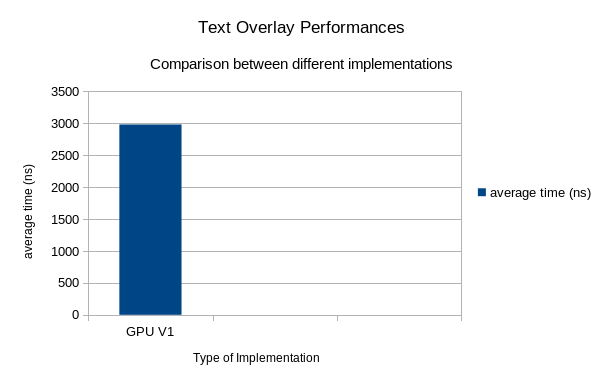
\includegraphics[width=0.9\linewidth]{images/chart7.png}
		\caption{\textit{Text Overlay Comparison}}
		\label{fig:chart7}
	\end{figure}

	\subsubsection{Exploiting the global memory access optimization}

	It's possible then to optimize the kernel from the point of view of the global memory access parallelism as explained in Section \ref{sec:cherry}. By copying and modifing the same kernel structure, the resulting kernel is:

	\begin{lstlisting}[style=CStyle]
typedef long4 chunk_t;

__global__ void kernel2_char(
uint8_t *current, uint8_t *matrix, int N, int offset, 
int matrixWidth, int currWidth) {
    int thid = threadIdx.x + blockIdx.x * blockDim.x;
    chunk_t cc;

    int start = thid * N;
    int max = start + N;

    for (int i = start; i < max; i++) {
        int reali = i * sizeof(chunk_t);
        int x = offset + reali % matrixWidth;
        int y = reali / matrixWidth;

        int idx = (y * currWidth + x) / sizeof(chunk_t);
        cc = ((chunk_t *)current)[idx];

        #pragma unroll
        for (int j = 0; j < sizeof cc; j++) {
            ((uint8_t *)&cc)[j] = matrix[reali + j];
        }

        ((chunk_t *)current)[idx] = cc;
    } 
	\end{lstlisting}

	
	By running the profiler for a fixed time of 30 seconds, the kernel takes an average time of 3.778 us so it occupies the 1.91\% of the total time.\\

	A comparison chart is show in Figure \ref{fig:chart8}:

	\begin{figure}[H]
		\centering
		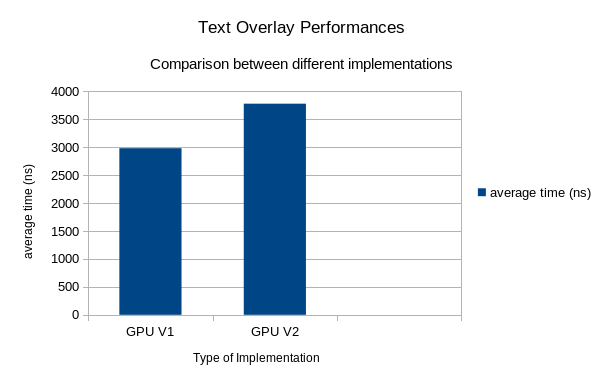
\includegraphics[width=0.9\linewidth]{images/chart8.png}
		\caption{\textit{Text Overlay Comparison}}
		\label{fig:chart8}
	\end{figure}

	As noticeable, the performance are worse. This is because the intermediate \textit{for loop} can be compacted in a single instruction because it's only an assignment without other operations in the middle. The new kernel is then shorter and faster, as follow:

	\begin{lstlisting}[style=CStyle]
typedef long4 chunk_t;

__global__ void kernel2_char(
uint8_t *current, uint8_t *matrix, int N, int offset, 
int matrixWidth, int currWidth) {
    int thid = threadIdx.x + blockIdx.x * blockDim.x;
    chunk_t cc;

    int start = thid * N;
    int max = start + N;

    for (int i = start; i < max; i++) {
        int reali = i * sizeof(chunk_t);
        int x = offset + reali % matrixWidth;
        int y = reali / matrixWidth;

        int idx = (y * currWidth + x) / sizeof(chunk_t);
        ((chunk_t *)current)[idx] = ((chunk_t *)matrix)[i];
    } 
	\end{lstlisting}

	By running the profiler for a fixed time of 30 seconds, the kernel takes an average time of 1.868 us so it occupies the 1.01\% of the total time. This means that the last version of the kernel is faster than the first one.\\

	A comparison chart is show in Figure \ref{fig:chart9}:

	\begin{figure}[H]
		\centering
		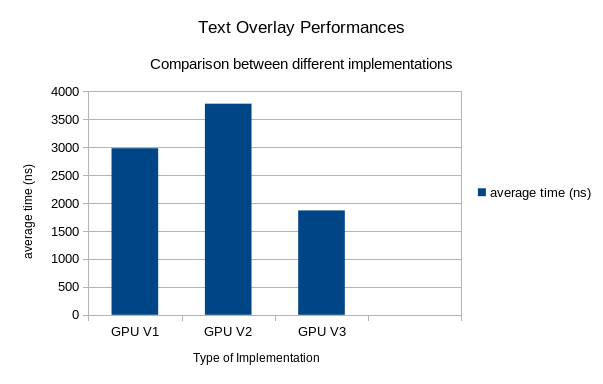
\includegraphics[width=0.9\linewidth]{images/chart9.png}
		\caption{\textit{Text Overlay Comparison}}
		\label{fig:chart9}
	\end{figure}

	\subsubsection{Constant Memory instead of Global Memory: is it worth?}

	Because character frames are basically constant during the execution of the program, is it really necessary to use the global memory or another kind of memory can be exploited? If yes, is it really worth? \\

	For this kind of purposes, CUDA devices offer the so called Constant Memory, that is a piece of memory on the GPU side that is constant. Because it's \textit{constant} from the GPU point of view but it can modified by the Host, it seems to be perfect for this part of the project.\\

	Usually it's large \textit{64 KB} so supposing to have an alphabet whose frames doesn't exceed this memory limit, a constant variable (array) can be declared and initialized as follows:

	\begin{lstlisting}[style=CStyle]
__constant__ uint8_t c_matrix[(sizeof(CHARS_STR) - 1) * 3 * 32 * 28];

uint8_t *c_matrixPtr;
cudaMemcpyToSymbol(c_matrix, charsPx, totcpy);
cudaGetSymbolAddress((void **)&c_matrixPtr, c_matrix);
\end{lstlisting}

Leaving \texttt{kernel2\_chars} as it is and using \texttt{c\_matrixPtr} instead of \text{d\_charsPx} in the kernel call and running the profiler, an unexpected value is returned by the profiler. The exeuction time is almost the same (faster only for a few nanoseconds) than the previous implementation and this is due to two reasons mainly:

\begin{enumerate}
	\item the kernel is instruction-bound and not memory-bound
	\item according to CUDA's programming guide: "\textit{For all threads of a half-warp, reading from the constant cache is as fast as reading from a register as long as all threads read the same address. The cost scales linearly with the number of different addresses read by all threads.}". This means that the shared memory is really faster than the global memory but becuase the kernel is accessing every time a different address, the cost of access increases by reaching the cost of the global memory.
\end{enumerate}

A comparison chart is show in Figure \ref{fig:chart10}:

	\begin{figure}[H]
		\centering
		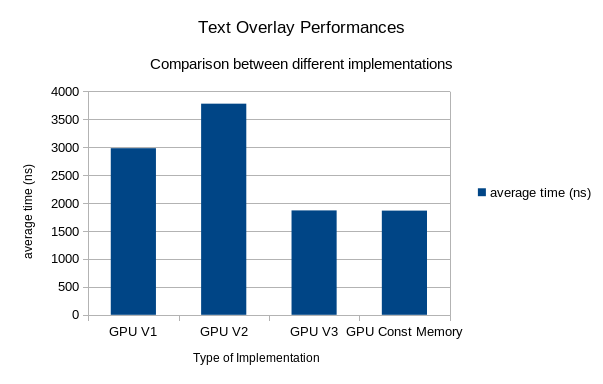
\includegraphics[width=0.9\linewidth]{images/chart10.png}
		\caption{\textit{Text Overlay Comparison}}
		\label{fig:chart10}
	\end{figure}


	\section{HeatMap}
	Since the basis of this project is to send the pixel difference, the lower the dissimilarities the higher the bandwidth saving. In order to better visualize which pixels changes the most and the different magnitudes, an heatmap is generated with the current and the previous frames.\newline\newline	
	A heat map is nothing else than a data visualization technique that represents the magnitude of a measurement as colors in two dimensions, in this case an image. The idea is first compute the difference at the pixel level between two successive frames and then represent it using a color scale from blue to red, where blue means low difference and red high difference. The Image \ref{fig:heat_v0} shows a naif implementation of heat map, available at \texttt{heat\_map\_benchmark/v0.cu}, that generates in real time the image on the right.

	\begin{figure}[H]
		\centering
		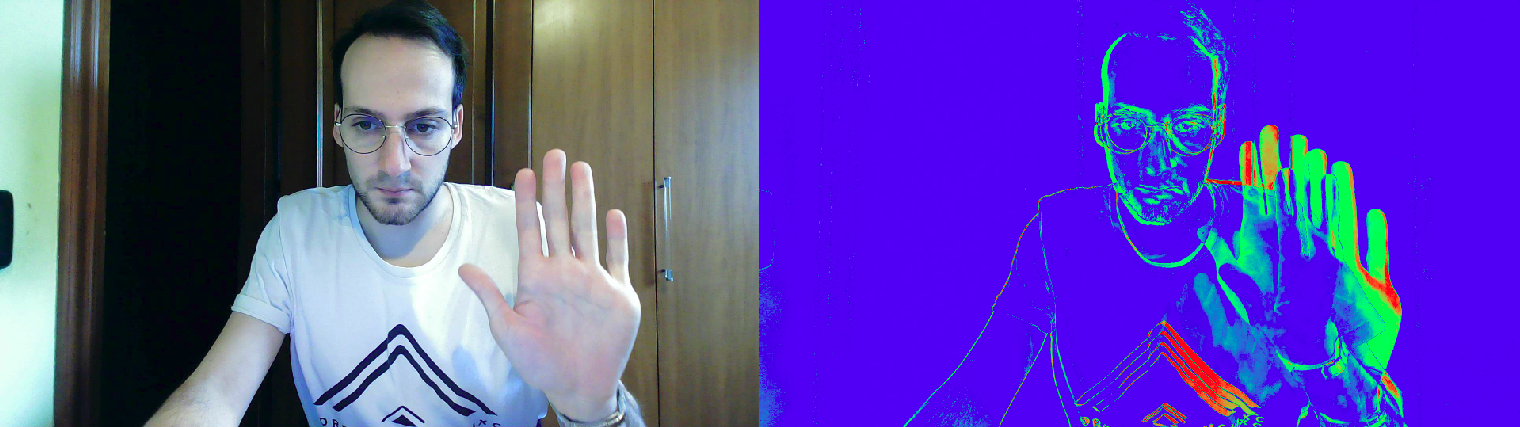
\includegraphics[width=0.9\linewidth]{images/heatmap/v0}
		\caption{\textit{Example of real-time heat map from webcam}}
		\label{fig:heat_v0}
	\end{figure}
	The basic steps for generating an heat map are the following:
	\begin{itemize}
		\itemsep0sp
		\item Take two frames from the webcam via OpenCV
		\item Compute the pixel difference
		\item Translate the difference into the corresponding color for the heat map
		\item Copy the result into a support buffer image and visualize it
	\end{itemize}
	All programs versions for the heat map are available in the \texttt{heat\_map\_benchmark} folder.
	
	\subsection{Heat map pixel mapping - CPU Naif implementation}
	
	The first \textit{naif} version has been done on the CPU. This implementation can generate an heatmap in more or less 980ms, that is too much. This is also due to the complexity of the function itself that is used to map a normalized pixel difference to a blue-red scale and because the image is sequentially analyzed.
	In order to convert the difference of a pixel into the three color component (RGB), the usage of the \textit{sine} function has been done. The difference of the each pixel has been computed as the sum of the absolute value of the difference of the single color component, as:
	\[
		diff = abs(Previous[i,R] - Curr[i,R]) + abs(Previous[i,G] - Curr[i,G] + abs(Previous[i,B] - Curr[i,B])
	\]
	Where $Previous[i,R]$ is the pixel red color component of the pixel at index $i$. In the worst case, a pixel can be turned from black to white or vice versa and so, the $0 \leq diff \leq 765$, that is $255 \cdot 3$. Then the $diff$ value is taken and normalize, by using 765 so that, $0 \leq diff_{norm} \leq 1$.:
	\[
		diff_{norm} = \frac{diff}{765}
	\]
	
	This value must be mapped into the tree RGB component of the heat map; the pixel must be more blue if the difference is more toward 0.0, yellow/green if near 0.5 and red if next to 1.0.
	The smoothed way to perform this task is to use three different sine functions, centered respectively on 0.0, 0.5 and 1.0 as in the following way:
	\begin{align*}
		\text{RED    } & \quad sin(\pi \cdot diff_{norm} - \frac{\pi}{2.0})\\
		\text{GREEN  } & \quad sin(\pi \cdot diff_{norm})\\
		\text{BLUE   } & \quad sin(\pi \cdot diff_{norm} + \frac{\pi}{2.0})
	\end{align*}
	The plot of the three sine functions is available at Figure \ref{fig:heat_sine}.

	 
	\begin{figure}[H]
		\centering
		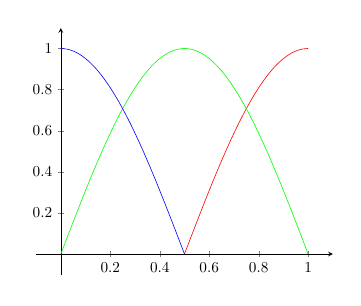
\begin{tikzpicture}[scale=0.55]
			\begin{axis}[
				trig format plots=rad,
				axis lines = middle,
				enlargelimits,
				clip=false
				]
				\addplot[domain=0.5:1,samples=200,red] {sin(pi*x - pi/2.0)};
				\addplot[domain=0:1,samples=200,green] {sin(x*pi)};
				\addplot[domain=0:0.5,samples=200,blue] {sin(pi*x + pi/2.0)};
				
			\end{axis}
		\end{tikzpicture}
	\caption{\textit{Mapping function from pixel difference to RGB components}}
	\label{fig:heat_sine}
	\end{figure}
	The CPU implementation is the following:
	\begin{lstlisting}[style=CStyle]
struct HeatElemt {
	int r;
	int g;
	int b;
};

HeatElemt getHeatPixel(int diff){
	struct HeatElemt h;
	float diff1 = diff/(255.0*2.0);
	
	// Map the difference into the three color components
	h.r = min(max(sin(M_PI*diff1 - M_PI/2.0)*255.0, 0.0),255.0);
	h.g = min(max(sin(M_PI*diff1)*255.0, 0.0),255.0);
	h.b = min(max(sin(M_PI*diff1 + M_PI/2.0)*255.0, 0.0),255.0);
}

while (1) {
	cap >> image2;
	for (int y = 0; y < H; y++){
		for (int x = 0; x < W; x++){
			Vec3b & intensity = image1.at<Vec3b>(y, x);
			Vec3b a = image1.at<Vec3b>(y, x);
			Vec3b b = image2.at<Vec3b>(y, x);
			
			// Compute the absolute difference
			HeatElemt elem = getHeatPixel(abs(a.val[0] - b.val[0]) + 
			abs(a.val[1] - b.val[1]) + abs(a.val[2] - b.val[2]));
			
			intensity.val[0] = elem.b;
			intensity.val[1] = elem.g;
			intensity.val[2] = elem.r;
		}
	}
	image1 = image2.clone();
}\end{lstlisting}
	In this CPU implementation, a loop is performed over each pixel of the two frames and the absolute difference computed. Another function, called \texttt{getHeatPixel} is used to convert that value to the heat map RGB color space. At this point, the original image is overwritten with the heatmap colors.

	
	\subsection{CUDA implementation}
	
	The idea is to rewrite what described in the previous section into a CUDA code. The GPU allows to run in parallel multiple instance of the same kernel, so that the execution can be done in parallel in order to speed up the computation.
	
	From the perspective of the interaction, the GPU acts like an accelerator of the CPU, that ask it to execute the kernel by resorting to the following phases:
	\begin{enumerate}
		\itemsep0sp
		\item Copy the frames from the Host to the Device memory
		\item Execute the kernel and wait its completion
		\item Retrieve the result from the Device to the Host memory
	\end{enumerate}
	
	This is exactly what the next section will explain. The kernel call allows to configure how many thread per kernel will be executed; obviously, depending on that number, the accessed locations must be defined accordingly. In fact, by defining $K$ the number of thread lunched, each thread will work on a specific portion of the entire image:
	\[
		\text{Thread portion dimension} = \frac{W \cdot H \cdot 3}{K}
	\]
	Where $W$ and $H$ are the width and height of the image. The multiplication by 3 depends on the fact that each pixels is defined by three \texttt{uint8\_t} datatype that each one of them defines a specific color. \newline\newline
	Furthermore, from the memory allocation perspective of the GPU, the memory for the two frames and the heat map must be allocated. This is done only once at the startup of the program, thanks to the CUDA API.	

\begin{lstlisting}[style=CStyle]
// Pointer definition
uint8_t *d_current, *d_previous;
uint8_t *d_heat_pixels;	

// Memory space reservion on GPU	
cudaMalloc((void **)&d_current, W*H*C * sizeof *d_current);
cudaMalloc((void **)&d_previous, W*H*C * sizeof *d_previous);
cudaMalloc((void **)&d_heat_pixels, W*H*C * sizeof *d_heat_pixels);\end{lstlisting}

	Unfortunately, this type of the problem doesn't need any shared or constant memory because each location in the image (all three colors of all pixels) are accessed only once and using a shared memory would have only reduced the performance due to the overhead of the useless copy. Moreover, there are no data that are constant.
	
	CUDA allows to get the information about the maximum number of thread by using the \texttt{cudaGetDeviceProperties} command and, by referring to the equation defined before, $K$ can be set to that value. In fact, the kernel is launched with the following configuration:
	\begin{itemize}
		\itemsep0sp
		\item \textit{Grid dimensions}:  1, 0, 0
		\item \textit{Block dimensions}: $K$, 0, 0
	\end{itemize}
	Having the maximum number of threads in the \texttt{threads} variable, it's possible to call the kernel in the following way:
	\begin{lstlisting}[style=CStyle]
// Kernel per block computation
cudaGetDeviceProperties(&prop, 0);
int threads = prop.maxThreadsPerBlock;
int maxSection = (W*H*C)/threads;\end{lstlisting}
	
	An extensive analysis of the correct number of threads has been done at Section \ref{sec:thread_n}.

	\subsubsection{CUDA Naif implementation}
	The first implementation of the algorithm in CUDA is based on a 1:1 transposition of what done in the CPU, in the GPU. Always using OpenCV, two next frames are fetched, send to the kernel and the heat map computed.
	
	\begin{lstlisting}[style=CStyle]
// Copy from Host to Device
cudaMemcpy(d_prev, image1,  W*H*C * sizeof *image1, cudaMemcpyHostToDevice);
cudaMemcpy(d_curr, image2,  W*H*C * sizeof *image2, cudaMemcpyHostToDevice);

kernel<<<1, threads>>>(d_curr, d_prev, (W*H*C)/threads, d_out);

// Copy heat map from Device to Host
cudaMemcpy(heatmap, d_out, W*H*C * sizeof *heatmap, cudaMemcpyDeviceToHost);\end{lstlisting}

	This naif implementation implies two memory transfers (HostToDevice) for the previous and current frames and one DeviceToHost for the generated heat map.
	
	
	In order to speed up the data management, instead of copying into a support array of \texttt{uint8\_t} the entire two frames (previous and current), both frames are directly copied into the device buffers with the \texttt{cudaMemcpy} procedure.\newline\newline
	Form the kernel perspective, there is a non-negligible complication with the respect to the CPU implementation. The CPU code is based on a single thread that iterates over the entire image in a sequential way, accessing one location after the other. For the GPU this is not the case, since now, each thread will work in parallel on a portion of the image that is long \texttt{maxSect}.
	
	Due to this, each kernel must know exactly from which pixel start to retrieve the data and where to store the results. This is only a matter of index management; let's suppose to have frame with dimension 1920*1080*3. So, by using 1024 threads per block, each thread will work on:
	\[
		maxSect = \frac{1920*1080*3}{1024} = 6075
	\]
	This means that the first thread must work from 0 to 6074, the second one from 6075 to 12149 and so on. This can be simply achieved by giving an univocal index identifier to each kernel, that cam be generated as:\newline\newline
	\texttt{int x = threadIdx.x + blockDim.x * blockIdx.x;}\newline\newline
	The GPU implementation of the first CUDA kernel is the following:
	\begin{lstlisting}[style=CStyle]
__global__ void kernel(uint8_t *current, uint8_t *previous,
					int maxSect, uint8_t* d_heat_pixels) {
	
	// Index relative to the block					
	int x = threadIdx.x + blockDim.x * blockIdx.x;
	
	// Start of the sector for this thread
	int start = x * maxSect;
	int max = start + maxSect;
	for (int i = start; i < max; i=i+C) {
		
		// Compute the pixel difference
		int pixelDiff = fabsf(current[i] - previous[i]) + fabsf(current[i+1]
				- previous[i+1]) + fabsf(current[i+2] - previous[i+2]); 
		float diff1 = pixelDiff/(255*3.0);
		
		// Map different into the three color component
		int r = fminf(fmaxf(sinf(M_PI*diff1 - M_PI/2.0)*255.0, 0.0),255.0);
		int g = fminf(fmaxf(sinf(M_PI*diff1)*255.0, 0.0),255.0);
		int b = fminf(fmaxf(sinf(M_PI*diff1 + M_PI/2.0)*255.0, 0.0),255.0);
		d_heat_pixels[i] = b;
		d_heat_pixels[i+1] = g;
		d_heat_pixels[i+2] = r;
	}
} \end{lstlisting}
	
	After having run the \texttt{nvprof}, the main contributions to the execution time from the profiler are:
	\begin{table}[H]
		\centering
			\begin{center}
			\begin{tabular}{ |c|c|c|c| } 
				\hline
				\textbf{Type} & \textbf{Time} (\%) & \textbf{Avg} & \textbf{Name} \\ 
				\hline
				GPU activities & 86.14 & 49.958 & kernel \\ 
				& 9.38 & 2.5577ms & [CUDA memcpy HtoD] \\ 
				& 4.48 & 2.4427ms & [CUDA memcpy DtoH] \\ 
				\hline
				API calls & 93.88 & 18.820ms & cudaMemcpy \\ 
				& 5.88 & 181.61ms & cudaMalloc \\ 
				\hline
			\end{tabular}
		\end{center}
		\label{fig:table_v1}
		\caption{\textit{Profiling result v1.cu}}
	\end{table}
	In fact, the cumulative time needed to copy all two frames into the device, execute the kernel and copy back the image in order to display it, takes approximately 57ms. From the GPU perspective, the average time to execute one single kernel is 49.958ms.
	
	
	
	\begin{figure}[H]
		\centering
		\begin{center}
			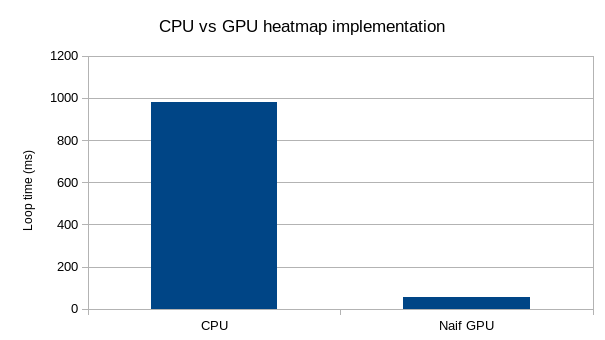
\includegraphics[width=0.6\linewidth]{images/heatmap/gpu_naif}
		\end{center}
	\label{fig:cpu_vs_gpu}
	\caption{\textit{Loop time CPU vs GPU}}
	\end{figure}
	
	\subsubsection{CUDA switching frames}
	
	The first idea to reduce the time used for copying the frames from the Host to the Device. Instead of copying each time both the two frame, one of the two can be reused by only switching the two points, so that the one that previously was the current will became the previous; at this point, only the new frame must be copied into the device memory. This means that approximately the \textit{CUDA memcpy HtoD} should be half of the previous time. This led to a \texttt{v2.cu} implementation, that exploit this pointer switching to reduce the memory transfer. The below code portion shows only the pointer switching in the loop used to fetch the frames.
		\begin{lstlisting}[style=CStyle]
while(1){
	// New frame fetch
	cap >> image2;
	
	// Pointer switching
	uint8_t* tmp = d_curr;
	d_curr = d_prev;
	d_prev = tmp;
	
	// Kernel call
	cudaMemcpy(d_curr, image2,  W*H*C * sizeof *image2, cudaMemcpyHostToDevice);
	kernel<<<1, threads>>>(d_curr, d_prev, (W*H*C)/threads, d_out);
	cudaMemcpy(heatmap, d_out, W*H*C * sizeof *heatmap, cudaMemcpyDeviceToHost);
	
	image1 = image2.clone();
}\end{lstlisting}
	
	\begin{table}[H]
		\centering
		\begin{center}
			\begin{tabular}{ |c|c|c|c| } 
				\hline
				\textbf{Type} & \textbf{Time} (\%) & \textbf{Avg} & \textbf{Name} \\ 
				\hline
				GPU activities & 90.54 & 46.023 & kernel \\ 
				& 4.85 & 2.4400ms & [CUDA memcpy HtoD] \\ 
				& 4.61 & 2.3453ms & [CUDA memcpy DtoH] \\ 
				\hline
				API calls & 89.88 & 26.026ms & cudaMemcpy \\ 
				& 9.90 & 192.15ms & cudaMalloc \\ 
				\hline
			\end{tabular}
		\end{center}
		\label{fig:table_v2}
		\caption{\textit{Profiling result v2.cu}}
	\end{table}
	The average kernel execution time is in ms, and it is not a figure of interest, since it is more or less equal to the previous version. What is important is that now, the percentage of time used for the kernel is increase, due to the reduced \textit{CUDA memcpy HtoD} (from  9.38\% to 4.85\%). This means that the GPU will analyze more frame in the same time frame. As we would expect, now the time needed to copy a frame from the memory to the device, execute the kernel and then retrieve the heat map takes about 50ms (12\% faster).
	
	\begin{center}
		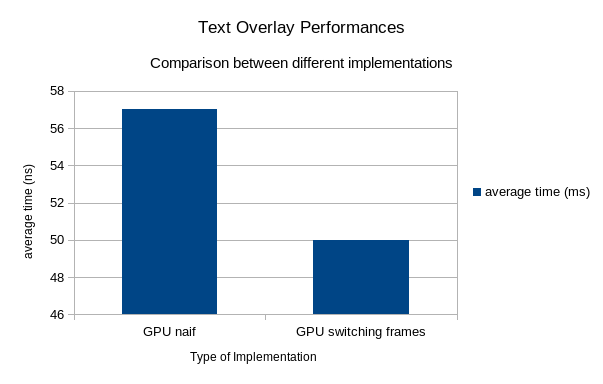
\includegraphics[width=0.6\linewidth]{images/heatmap/comp_heat_3}
	\end{center}
	
	
	\subsubsection{CUDA Global memory access granularity}
	The problem with the generation of the heat map is that, the computation of the color must be done every time for all the pixels in order to compute the complete image.\newline\newline
	Since each thread must perform 6075 iterations and need to write on the Global memory the same amount of times.
	In order to reduce the number of accesses to the Global memory, the idea was to access at the \texttt{int} level instead of the \texttt{byte} level. This means that frame information are still copied from host to device as arrays of \textit{bytes} but they are accesses at the int level. So, if the current and the previous frames are passed as \texttt{uint8\_t *current, uint8\_t *previous}, the access is aligned at the 4 bytes. 
	Another problem arises: the threads now access the memory with a granularity of 4 byte, but since the pixel difference needs needs only the first three bytes (RGB), in order to optimize and avoid to read twice from the memory, colors are updated only once every 3 bytes. So, when the position of the color in the image is the first, the colors of the heat map are set in the current and next two bytes of the output array, accordingly to the computed difference.
	\begin{lstlisting}[style=CStyle]
__global__ void kernel(uint8_t *current, uint8_t *previous,
					int maxSect, uint8_t* d_heat_pixels) {
	int x = threadIdx.x + blockDim.x * blockIdx.x;
	int start = x * maxSect;
	int max = start + maxSect;
	int cc, pc;
	for (int i = start; i < max; i++) {
		
		// Access one 4 byte at a time
		cc = ((int *)current)[i];
		pc = ((int *)previous)[i];
		int pixelDiff = 0;
		for (int j = 0; j < 4; j++) {
			
			// Conversion from difference to heat map only every 3 bytes
			if((i*4+j) % 3 == 0){
				int pixelDiff = fabsf(((uint8_t *)&cc)[j] - ((uint8_t *)&pc)[j]) +
				fabsf(((uint8_t *)&cc)[j+1] - ((uint8_t *)&pc)[j+1]) +
				fabsf(((uint8_t *)&cc)[j+2] - ((uint8_t *)&pc)[j+2]);
				float diff1 = pixelDiff/(255*2.0);
				int r = fminf(fmaxf(sinf(M_PI*diff1 - M_PI/2.0)*255.0, 0.0),255.0);
				int g = fminf(fmaxf(sinf(M_PI*diff1)*255.0, 0.0),255.0);
				int b = fminf(fmaxf(sinf(M_PI*diff1 + M_PI/2.0)*255.0, 0.0),255.0);
				d_heat_pixels[i*4+j] = b;
				d_heat_pixels[i*4+j+1] = g;
				d_heat_pixels[i*4+j+2] = r;
				
				// Reset the pixel difference
				pixelDiff = 0;
			}
		}
	}
}\end{lstlisting}
	Since now each threads works on 4 bytes at a iteration, the dimension of the data section that each block must work on is reduced by $1/4$, as in the following way:
		\begin{lstlisting}[style=CStyle]
cudaGetDeviceProperties(&prop, 0);
int threads = prop.maxThreadsPerBlock;

cudaMemcpy(d_curr, image2,  W*H*C * sizeof *image2, cudaMemcpyHostToDevice);

// Kernel call /4
kernel<<<1, threads>>>(d_curr, d_prev, ((W*H*C)/threads)/4, d_out);
cudaMemcpy(heatmap, d_out, W*H*C * sizeof *heatmap, cudaMemcpyDeviceToHost);\end{lstlisting}

	This led to another version, available at \texttt{v3.cu} allows to obtain the following results:
	\begin{table}[H]
		\centering
		\begin{center}
			\begin{tabular}{ |c|c|c|c| } 
				\hline
				\textbf{Type} & \textbf{Time} (\%) & \textbf{Avg} & \textbf{Name} \\ 
				\hline
				GPU activities & 84.08 & 25.457ms & kernel \\ 
				& 8.14 & 2.4405ms & [CUDA memcpy HtoD] \\ 
				& 7.78 & 2.3549ms & [CUDA memcpy DtoH] \\ 
				\hline
				API calls & 85.73 & 15.810ms & cudaMemcpy \\ 
				& 13.93 & 172.12ms & cudaMalloc \\ 
				\hline
			\end{tabular}
		\end{center}
		\label{fig:table_v3}
		\caption{\textit{Profiling result v3.cu using int access level}}
	\end{table}
	
	This version allows to copy the next frame from memory to device, execute the kernel and retrieve the result in about 30ms (about 40\% of performance increase from \texttt{v2.cu}). This is highlighted in the table by the average time needed to execute the kernel itself, we went from 46.023ms to 25.457ms, thanks to the reduce access time to the memory.
	
	\begin{center}
		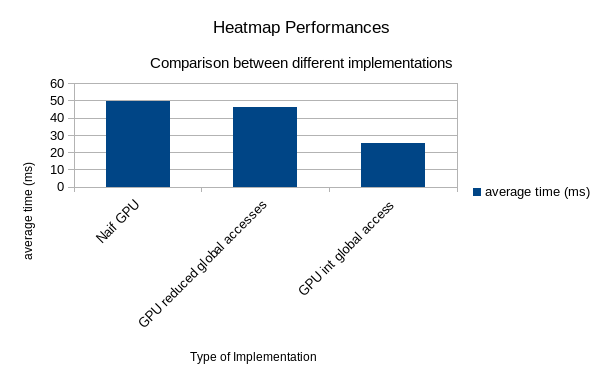
\includegraphics[width=0.6\linewidth]{images/heatmap/comp_heat_4}
	\end{center}
	
	This can be pushed even more, so that instead of accessing the images that are in the global memory, at the \texttt{int} level, they are accessed via a vectorized access. The complete explanation is available at Section \ref{sec:cherry}. By the way, it is able to increase even more the performance, allowing to complete the for loop in around 27ms using \texttt{long4} data type.
		\begin{table}[H]
		\centering
		\begin{center}
			\begin{tabular}{ |c|c|c|c| } 
				\hline
				\textbf{Type} & \textbf{Time} (\%) & \textbf{Avg} & \textbf{Name} \\ 
				\hline
				GPU activities & 82.83 & 23.589ms & kernel \\ 
				& 8.92 & 2.5160ms & [CUDA memcpy HtoD] \\ 
				& 8.24 & 2.3478ms & [CUDA memcpy DtoH] \\ 
				\hline
				API calls & 85.42 & 14.903ms & cudaMemcpy \\ 
				& 14.18 & 165.80ms & cudaMalloc \\ 
				\hline
			\end{tabular}
		\end{center}
		\label{fig:table_v5}
		\caption{\textit{Profiling result v3.cu using long4 access level}}
	\end{table}
	\begin{center}
		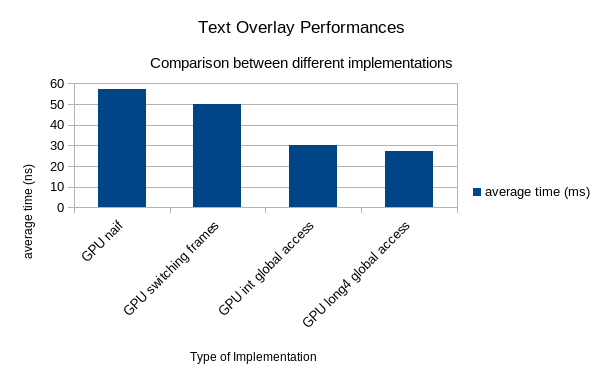
\includegraphics[width=0.6\linewidth]{images/heatmap/comp_heat_5}
	\end{center}
	
	
	\subsection{Evaluation of the number of threads}
	\label{sec:thread_n}
	For a first implementation, the number of thread has been set to the maximum allowable from the architecture, that is given by the \texttt{cudaGetDeviceProperties} CUDA function in order to make the program independent form the device used. For example, for the Jetson Nano, the maximum number of threads are 1024.\newline\newline
	In order to understand how the number of threads impacts on the heat map generation, a bash script has been build in order to dynamically change the $K$ parameter via compiler directive. The number of threads must be a multiple of 4, so that the array of the pixels can be divided into portion in such a way that a pixel is not split between two kernel.
	
	This is the bash code used to extract the \textit{nvprof} information:
	\begin{lstlisting}[language=bash]
#!/bin/bash
for i in {1..256}
do
	k=$(( 4*i ))
	
	# Profiler call
	avg=`sudo /usr/local/cuda/bin/nvprof ./heatMap $k 2>&1`
	
	# Data extraction
	kern=`echo "$avg" | grep kernel | awk '{print $6}'`
	kernt=`echo "$avg" | grep kernel | awk '{print $4}'`
	hd1=`echo "$avg" | grep "CUDA memcpy HtoD" | awk '{print $4}'`
	hd2=`echo "$avg" | grep "CUDA memcpy HtoD" | awk '{print $2}'`
	dh1=`echo "$avg" | grep "CUDA memcpy DtoH" | awk '{print $4}'`
	dh2=`echo "$avg" | grep "CUDA memcpy DtoH" | awk '{print $2}'`
	echo "$k $all $kern $kernt $hd1 $hd2 $dh1 $dh2" >> times.txt
done\end{lstlisting}
	In this way, the output of the profiler and the time needed to copy the frame, generate the heat map and retrieve the result is parsed and wrote into a file called \texttt{times.txt}. Thanks to another script, the most useful data are plot, as below:
	
	\begin{figure}[H]
		\centering
		\begin{subfigure}{.45\textwidth}
			\centering
			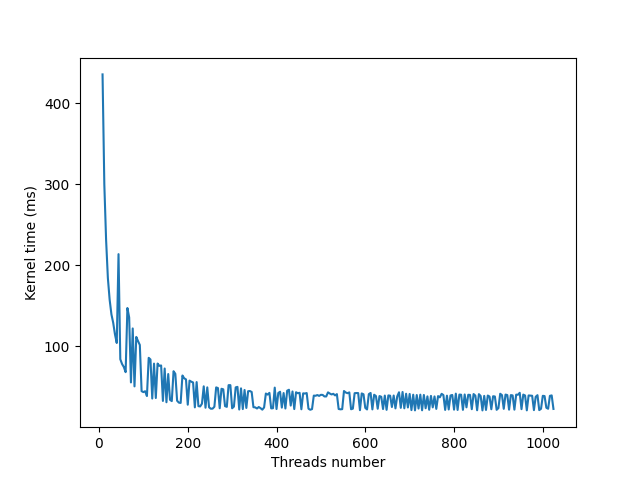
\includegraphics[width=1\linewidth]{images/heatmap/plot_kernel_times.png}
			\caption{Time needed to perform an heatmap depending on the number of kernel set}
			\label{fig:sub1}
		\end{subfigure}%
		\hspace{5mm}
		\begin{subfigure}{.45\textwidth}
			\centering
			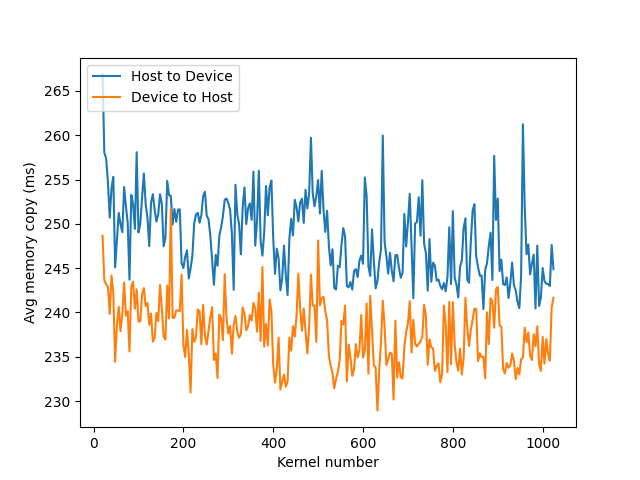
\includegraphics[width=1\linewidth]{images/heatmap/hd.png}
			\caption{Time needed to copy from Host to Device (blue) and from Device to Host (orange)}
			\label{fig:sub2}
		\end{subfigure}
	\end{figure}
	This is not the behaviour that we would have expected, beside the time needed to copy is more or less constant, by increasing the number of threads for that kernel we would expect that the time needed for the heat map computation would be lower. This is probably due to the fact that the \textit{warp} has a fixed size of 32 threads and, even if by increasing the number of threads its execution time is lower, their management probably introduce too much overhead to obtain benefits.
	
	Beside this, the time needed to perform an heatmap vs the number of threads, shows a peculiar behaviour. After about $N > 280$ the times tend to oscillate between more or less 50ms and 27ms. Even if this seems not a big difference, in the filed of real-time image processing, it's a huge improvement. In order to avoid errors, the same script has been run multiple times and the results is always the same. Since the internal infrastructure is a black box, the hardware probably manage in different ways the threads with the respect to their number.\newline
	The best observed thread configuration for the Jetson Nano, seems to be 716.\newline\newline
	In fact, by running the same exact algorithm describe before but the number of threads is set to 718 (that is the best kernel accordingly to the plot above), the time needed to copy a frame, compute the heat map and then copy back the heat map matrix is about 27ms. This leads to a increasing of performance of 10\%, that in this domain is not negligible.
	
	The following table shows some meaningful data extracted from the profiler:
		\begin{table}[H]
		\centering
		\begin{center}
			\begin{tabular}{ |c|c|c|c| } 
				\hline
				\textbf{Type} & \textbf{Time} (\%) & \textbf{Avg} & \textbf{Name} \\ 
				\hline
				GPU activities & 84.30 & 24.380ms & kernel \\ 
				& 8.04 & 2.4599ms & [CUDA memcpy HtoD] \\ 
				& 7.66 & 2.383ms & [CUDA memcpy DtoH] \\ 
				\hline
				API calls & 90.06 & 16.192ms & cudaMemcpy \\ 
				& 9.57 & 115.27ms & cudaMalloc \\ 
				\hline
			\end{tabular}
		\end{center}
		\label{fig:table_v4}
		\caption{\textit{Profiling result v3.cu}}
	\end{table}

	\subsubsection{Heatmap Conclusions}

	By considering only the CUDA algorithm, the optimizations shows a decreasing fashion of the time needed to process the two frames and generate the heat map. The Loop average time, is the time needed to copy the image from the Host to the Device, summed to the heat map time computation and the time needed to copy it back. On the other hand, the plot on the right shows only the average kernel time. All data are in ms. 
	\begin{center}
		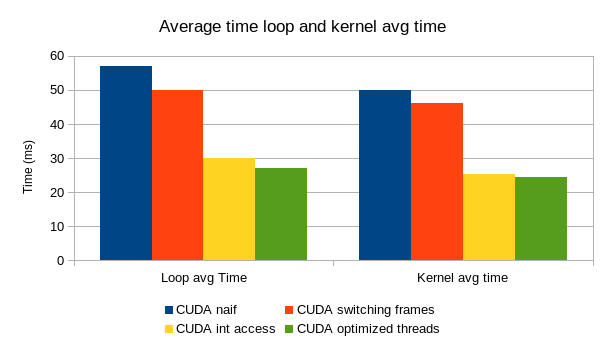
\includegraphics[width=0.65\linewidth]{images/heatmap/histo_results}
	\end{center}
	
	
	\section{Noise visualizer}
	\label{sec:noise_visualizer}
	As already explained in the first sections, the algorithm is based on sending only the difference of all pixels whose color components are above a certain threshold.
	
	In order to better visualize the noise in each frame taken from the webcam, all colors of all pixels that are above a certain threshold, are colored in red. The threshold is the same used by the kernel that computes all pixel differences. Obviously, the complexity of this computation is much easier than the previous one and the CPU allows to compute that kind of map in around 250ms.
	\begin{figure}[H]
		\centering
		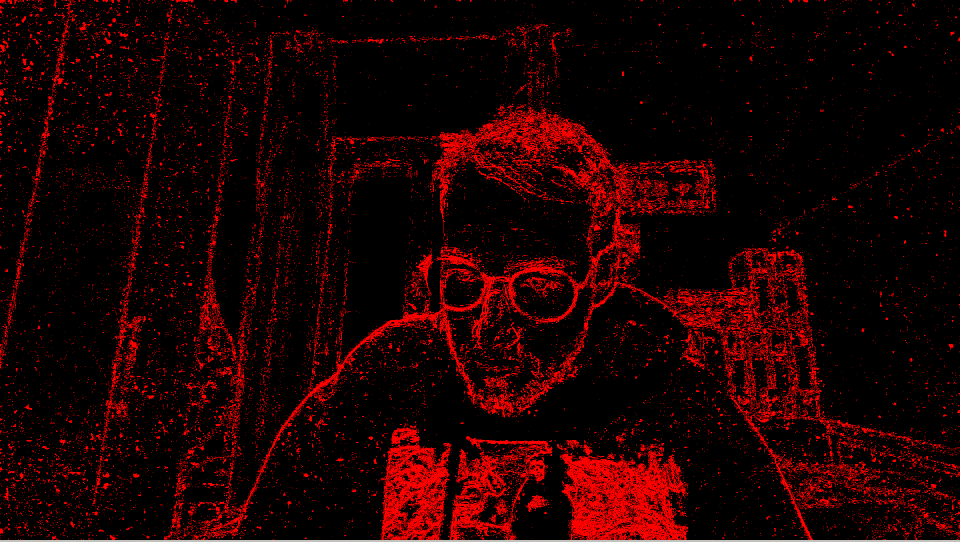
\includegraphics[width=0.4\linewidth]{images/heatmap/v0-red}
		\caption{\textit{All non normalized pixel difference are turned to red if above a certain threshold, in this case 20. Beside the figure in the center, all red pixels can be identified as noise.}}
		\label{fig:v0-red}
	\end{figure}
	The purpose of this new color mapping is completely different from the heatmap, since the latter one is used to understand the magnitude of the pixel difference while the second one (the black-red) is used to better visualize the noise pixels, by using a threshold.
	
	\textit{Why is this necessary?} This allows to have a visual evaluation of the noise filter, that is used to reduce smooth the noise in order to reduce the difference between two frames and reduce even more the bandwidth. The noise filter will be explained in the next section.\newline\newline
	First of all, we need to define what is the noise: by means of noise we are referring to all the random variations on the color information in an image, that is visible as grain in film and pixel level. The level of the noise mainly depends:
	\begin{itemize}
		\itemsep0sp
		\item Length of the exposure
		\item Sensitivity of the optical camera
		\item Brightness of the environment
		\item Temperature
	\end{itemize}
	In most of the cases, the webcam used at home is a cheap one that has an extremely small pixels in the camera sensor. There are mainly three types of noises: fixed pattern noise, random noise and banding noise. The common noise in our webcam is the one shown below. As you can see, the dark and less brightness parts of the image are characterized by some particles that shows different color from the whole context. 
	\begin{figure}[H]
		\centering
		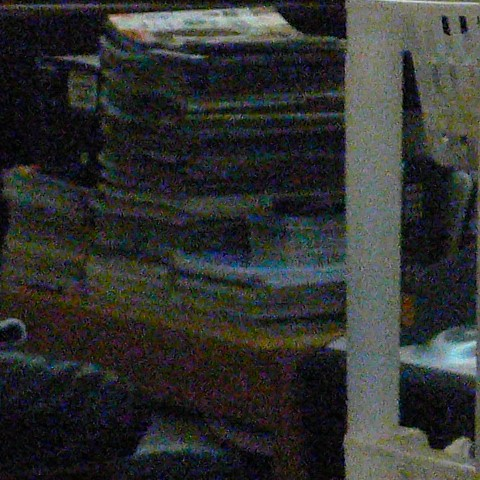
\includegraphics[width=0.25\linewidth]{images/heatmap/noise}
		\caption{\textit{Example of noise}}
		\label{fig:noise}
	\end{figure}
	From our perspective this is a very bad behaviour due to the fact that the noise is random, and can change the value of the pixel at each frame. This leads to an high amount of pixel changed, even if the image is always the same. For this reason, \textit{noise image filtering} is performed over the frame, before being analyzed by the CUDA kernel that computes the pixel differences.\newline\newline

	The internal logic of a webcam allows to trim some parameters of the video capture directly by OpenCV. This is not a software level manipulation of the frame, but the internal control unit of the webcam, while sampling the frame, performs different behaviour depending on the selected configuration. 
	
	For this reason, the original image has been enhanced with a control panel, so that the user can change the brightness, the contrast, the saturation and the gain of the image. The Figure \ref{fig:controls}, shows the panel that is shown to the user. Even if it can be used to reduce the noise, by for example reducing the contrast, it allows the user to increase the quality of the send image.
	\begin{figure}[H]
		\centering
		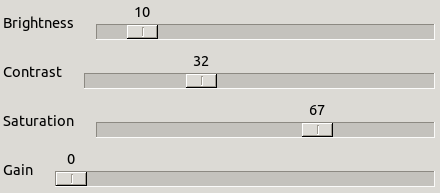
\includegraphics[width=0.33\linewidth]{images/heatmap/controls}
		\caption{\textit{Image Control panel}}
		\label{fig:controls}
	\end{figure}
	
	\subsubsection{Naif CPU implementation}
	The \textit{naif} CPU implementation starts from the same program base used for the heat map. The entire image, pixel by pixel, is analyzed and if one of the color component is above the same threshold set for the pixel difference, that pixel is colored in red otherwise in black.
	
	The code below is the C implementation of what explained before, where \texttt{LR\_THRESHOLDS} is set to 20.
\begin{lstlisting}[style=CStyle]
for (int y = 0; y < H; y++){
	for (int x = 0; x < W; x++){
		Vec3b & intensity = image1.at<Vec3b>(y, x);
		Vec3b a = image1.at<Vec3b>(y, x);
		Vec3b b = image2.at<Vec3b>(y, x);
		
		if(abs(a.val[0] - b.val[0]) > LR_THRESHOLDS ||
					abs(a.val[1] - b.val[1]) > LR_THRESHOLDS ||
					abs(a.val[2] - b.val[2]) > LR_THRESHOLDS)
		{
			intensity.val[0] = 0;
			intensity.val[1] = 0;
			intensity.val[2] = 255;
		} else {
			intensity.val[0] = 0;
			intensity.val[1] = 0;
			intensity.val[2] = 0;
		}
	}
}\end{lstlisting}
	The resulting image is the one at Figure \ref{fig:v0-red}. From the time perspective, as said before, being the operations for the noise visualizer less complex, the CPU is able to generate the image in around 250ms.
	
	\subsubsection{CUDA implementation}
	The same considerations and optimization steps done for the heat map can be done also for the generation of the frames that allows the user to better visualize the noise in the frames. So, starting from an already optimized memory management, the resulting kernel call is based as always on first copy the frame into the Device Global memory, call the kernel and then retrieve the image, as in the code below:
\begin{lstlisting}[style=CStyle]
	cudaGetDeviceProperties(&prop, 0);
	int threads = prop.maxThreadsPerBlock;
	
	cudaMemcpy(d_curr, image2,  W*H*C * sizeof *image2, cudaMemcpyHostToDevice);
	
	// Kernel call /4
	kernel_red<<<1, threads>>>(d_curr, d_prev, ((W*H*C)/threads/
																(sizeof(chunk_t)), d_out);
	cudaMemcpy(heatmap, d_out, W*H*C * sizeof *heatmap, cudaMemcpyDeviceToHost);\end{lstlisting}
	
	In this case, the optimization described in the pixel difference generation, regarding the \textit{vectorized access} to memory is also applied here, where a new type called \texttt{chunk\_t} is defined. In this way more byte can be read with a single memory access.
	
	\begin{lstlisting}[style=CStyle]
typedef int4 chunk_t;
	
__global__ void kernel_red(uint8_t *current, uint8_t *previous,
					int maxSect, uint8_t* d_heat_pixels) {
	    int x = threadIdx.x + blockDim.x * blockIdx.x;
	int start = x * maxSect;
	int max = start + maxSect;
	chunk_t cc, pc;
	uint8_t redColor = 0;
	int df;
	int size = sizeof(chunk_t);
	
	for (int i = start; i < max; i++) {
		cc = ((chunk_t *)current)[i];
		pc = ((chunk_t *)previous)[i];
		
		for (int j = 0; j < size; j++) {
			df = ((uint8_t *)&cc)[j] - ((uint8_t *)&pc)[j];
			
			if ((df < -LR_THRESHOLDS || df > LR_THRESHOLDS)){
				redColor = 255;
			}
			
			if(((i*size)+ j ) % 3 == 2){
			noise_visualization[(i*size)+j] = redColor;
			redColor = 0;
		} else {
			noise_visualization[(i*size)+j] = 0;
		}
	}
}	\end{lstlisting}
	By iteration on all the color components of all the pixels in the frame, the difference with the previous frame is checked. If it is above the threshold, the value of the red color for that pixel is set to 255. 
	
	Being the red component the third in a pixel, it is set accordingly to the \texttt{redColor} variable only if the \texttt{i*size + j \% 3 == 2} (the red color).\newline\newline
	This implementation allows to copy the frame from Host to Device, compute the noise visualization and retrieve back the image from Device to Host memory in around 26ms.
	
	The following table shows some meaningful data extracted from the profiler:
	\begin{table}[H]
		\centering
		\begin{center}
			\begin{tabular}{ |c|c|c|c|c|c| } 
				\hline
				\textbf{Type} & \textbf{Time} (\%) & \textbf{Avg} & \textbf{Min} & \textbf{Max} & \textbf{Name} \\ 
				\hline
				GPU activities & 81.38 & 21.759ms & 19.489ms & 32.942ms & kernel\_red \\ 
				& 9.59 & 2.5469ms & 2.2134ms & 6.8552ms & [CUDA memcpy HtoD] \\ 
				& 9.03 & 2.4141ms & 2.1828ms & 3.5408ms & [CUDA memcpy DtoH] \\ 
				\hline
				API calls & 87.41 & 13.992ms &  2.7579ms & 156.01ms & cudaMemcpy \\ 
				& 12.13 & 194.86ms  & 3.8501ms & 576.73ms & cudaMalloc \\ 
				\hline
			\end{tabular}
		\end{center}
		\label{fig:table_v1_red}
		\caption{\textit{Profiling result v1.cu for noise visualizer}}
	\end{table}
	As you can see, the average time needed to compute the kernel is less with the respect to the heat map. This is due to the simplicity of the function that only need to check the difference against a threshold. As you can see, the GPU acceleration has a huge impact over the computation.
	\begin{center}
		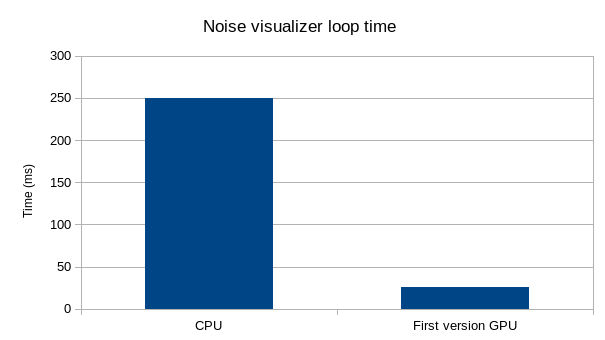
\includegraphics[width=0.35\linewidth]{images/heatmap/noise1}
	\end{center}
	
	
	\subsubsection{CUDA reduction of global memory accesses}
	The fact that the only pixels that changes is the red one, the previous CUDA kernel can be optimized even more in order to reduce the number of access to the global memory. In fact, if we set assume that at the beginning all pixels in the \texttt{d\_heat\_map} array are all completely black, the algorithm can reduce the memory access of on third since it will work only on a the red color component. As before, if the difference is above a threshold, the red pixel is turned to red, or to black otherwise.

	The resulting kernel is the following:
	
	\begin{lstlisting}[style=CStyle]
__global__ void kernel_red(uint8_t *current, uint8_t *previous,
	int maxSect, uint8_t* d_heat_pixels) {
		int x = threadIdx.x + blockDim.x * blockIdx.x;
		int start = x * maxSect;
		int max = start + maxSect;
		chunk_t cc, pc;
		uint8_t redColor = 0;
		int df;
		int size = sizeof(chunk_t);
		
		for (int i = start; i < max; i++) {
			cc = ((chunk_t *)current)[i];
			pc = ((chunk_t *)previous)[i];
			
			for (int j = 0; j < size; j++) {
				df = ((uint8_t *)&cc)[j] - ((uint8_t *)&pc)[j];
				
				if ((df < -LR_THRESHOLDS || df > LR_THRESHOLDS)){
					redColor = 255;
				}
				
				if(((i*size)+ j ) % 3 == 2){
				noise_visualization[(i*size)+j] = redColor;
				redColor = 0;
			}
		}
}	\end{lstlisting}
	As you can notice, the only difference is that the else condition is the last if statement has been removed. This means that the green and blue component are not modified, thus the global memory is left as is for these two bytes.
	
	This allowed to increase the performance of the kernel even more; as you can see from the table below the kernel now lasts in average 16.684ms, that is a 23\% faster. The entire loop is done in about 22ms. \newline\newline
	Moreover, the test must be performed in the same conditions because, depending on the video captured, it can show different number of changed pixels with the value of the difference above or below the threshold. For this reason, the \textit{nvprof} has been run while the webcam was covered with a black tape. Due to the fashion of the algorithm, also the minimum and maximum values have been included in the table below.

	\begin{table}[H]
		\centering
		\begin{center}
			\begin{tabular}{ |c|c|c|c|c|c| } 
				\hline
				\textbf{Type} & \textbf{Time} (\%) & \textbf{Avg} & \textbf{Min} & \textbf{Max} & \textbf{Name} \\ 
				\hline
				GPU activities & 75.63 & 16.684ms & 16.372ms & 35.942ms & kernel\_red \\ 
							   & 12.37 & 2.6294ms & 2.2265ms & 6.3841ms & [CUDA memcpy HtoD] \\ 
							   & 12.00 & 2.6294ms &  2.2265ms & 6.3841ms & [CUDA memcpy DtoH] \\ 
				\hline
				API calls & 86.00 &  11.610ms & 2.6999ms & 41.414ms & cudaMemcpy \\ 
						  & 13.56 & 183.71ms & 3.7352ms & 543.50ms & cudaMalloc \\ 
				\hline
			\end{tabular}
		\end{center}
		\label{fig:table_v2_red}
		\caption{\textit{Profiling result v2.cu for noise visualizer}}
	\end{table}

	\begin{center}
		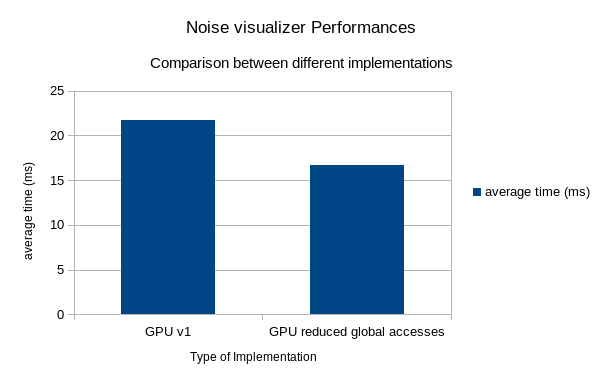
\includegraphics[width=0.6\linewidth]{images/heatmap/comp_heat_6}
	\end{center}


	The code of this and the previous implementation has been disassembled using the NVIDIA tools \textit{cuobjdump} and \textit{nvdisasm}; the last one is also needed to get information about the control flow. In order to avoid that the \textit{nvcc} compiler to avoid, with very limited exceptions, dead-code eliminations and register-spilling optimizations. For this reason the code has been compiled with the \texttt{-O0} flag.

	The generation of the assembly is:
	\begin{lstlisting}[language=bash]
cuobjdump ./a.out -xelf all
nvdisasm v1.sm_30.cubin\end{lstlisting}
	
	By looking carefully at the assembly code of the first implementation, it's possible to understand the correlation between the assembly code and the instructions. As we would have expected, in the code of the first implementation are present two \texttt{ST.E.U8} instructions, used to perform the if and else case.
	
	The following is an extract of the assembly that manage the if statement on the first CUDA implementation.
	\begin{figure}[H]
		\begin{lstlisting}[style=CStyle]
	// Perform comparison
	/*0ab0*/ ISETP.EQ.X.AND P0, PT, R5, RZ, PT;
	/*0ab8*/ PSETP.AND.AND P0, PT, !P0, PT, PT;
	/*0ac8*/ SSY `(.L_16);
	
	// Go to if
	/*0ad0*/ @P0 BRA `(.L_17);
	
	// Go to else
	/*0ad8*/ BRA `(.L_18);


// IF
.L_17
	...
	/*0e10*/ ST.E.U8 [R4], R0;
	/*0e28*/ NOP.S (*"TARGET= .L_16 "*);

// ELSE
.L_18:
	...
	/*0c50*/ ST.E.U8 [R4], R0;
	/*0c88*/ NOP.S (*"TARGET= .L_16 "*);


// Management of the loop control flow	
.L_16
	...\end{lstlisting}
	\caption{Assembly extract of the first CUDA implementation of the noise visualizer}
	\end{figure}

	So, label \texttt{.L\_17} and \texttt{.L\_18} are used to identify the branch that is used to write 0 or 255, accordingly to the fact that it is or not the red component and only if above the threshold.\newline\newline
	On the other hand, the assembly of the second implementation shows only one instance of the store byte instruction, as we would have expected:
	\begin{figure}[H]
	\begin{lstlisting}[style=CStyle]
	// Perform comparison
	/*0aa8*/ IADD32I RZ.CC, R4, -0x2;
	/*0ab0*/ ISETP.EQ.X.AND P0, PT, R5, RZ, PT;
	/*0ab8*/ PSETP.AND.AND P0, PT, !P0, PT, PT;
	/*0ac8*/ PRMT R0, R29, 0x7610, R0;
	/*0ad0*/ PSETP.AND.AND P0, PT, P0, PT, PT;
	/*0ad8*/ PRMT R0, R0, 0x7610, R0;
	/*0ae0*/ SSY `(.L_16);
	/*0ae8*/ @P0 NOP.S (*"TARGET= .L_16 "*);
	/*0af0*/ BRA `(.L_17);


// IF
.L_17
	...
	/*0e10*/ ST.E.U8 [R4], R0;
	/*0e28*/ NOP.S (*"TARGET= .L_16 "*);


// Management of the loop control flow	
.L_16
	...\end{lstlisting}
	\caption{Assembly extract of the second CUDA implementation of the noise visualizer}
	\end{figure}
	

	
	\subsubsection{Overlapping implementation}
	The fact that the we can have a frame that changes completely with the respect to the previous one, implies that not only the black pixels must be turned in red if above a certain threshold, but also the red ones that are below must be changed to black. This means that we if we have an image $1920*1080*3$ we can't go below $1920*1080$ access to Global Memory. 
	
	A second approach resort to not use the output \texttt{d\_heat\_pixels} as output array but instead write directly over the \textit{previous} frame. In this way, the red pixel will be placed over the frame itself; this is a completely different representation but, if we can modify the original frame (that will be discharged at the end of the loop), this solution is feasible. The result is visible at Figure \ref{fig:red_frame}.
	
	\begin{figure}[H]
		\centering
		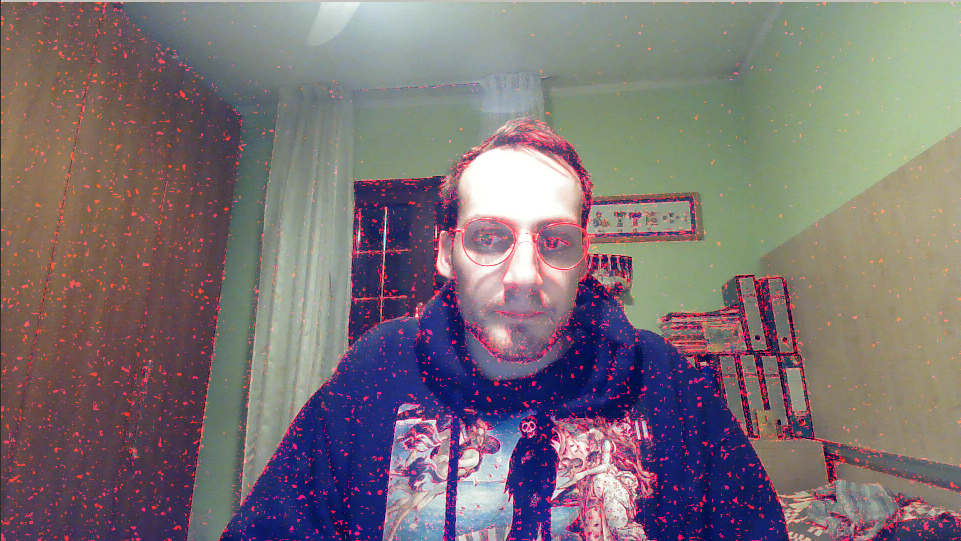
\includegraphics[width=0.45\linewidth]{images/heatmap/gpu_red_2}
		\caption{\textit{Red pixels over the frame}}
		\label{fig:red_frame}
	\end{figure}
	
	This has be done to overcome the need of setting a pixel to black when the difference between the pixels is below the threshold. With this approach, the number of write to the Global Memory should corresponds to the number of pixels whose difference is above the threshold. Hypothetically, two identical frames should not need any write access to the Global Memory.
	
	The kernel has been modified in the following way, so that the red color is set only if at least one color component of that pixel is above the threshold:
\begin{lstlisting}[style=CStyle]
__global__ void kernel_red(uint8_t *current, uint8_t *previous,
int maxSect) {
	int x = threadIdx.x + blockDim.x * blockIdx.x;
	int start = x * maxSect;
	int max = start + maxSect;
	chunk_t cc, pc;
	
	bool toUpdate = false;
	for (int i = start; i < max; i++) {
		
		cc = ((chunk_t *)current)[i];
		pc = ((chunk_t *)previous)[i];
		for (int j = 0; j < sizeof cc; j++) {
			int8_t df = ((uint8_t *)&cc)[j] - ((uint8_t *)&pc)[j];
			
			if (df < -LR_THRESHOLDS || df > LR_THRESHOLDS) {
				toUpdate = true;
			}
			
			// Update only if needed
			if (toUpdate && (i*(sizeof cc)+j) % 3 == 2){
			previous[i*(sizeof cc)+j] = 255;
			toUpdate = false;
		}
	}
}	\end{lstlisting}

	Obviously, also the kernel call must be modified, so that instead of copying back data from the \texttt{d\_heat\_map} the data are retrieved from the previous frame, that has been overwrite during the kernel execution:
	
\begin{lstlisting}[style=CStyle]
cudaMemcpy(d_current, image2.data,  W*H*C * sizeof *image2.data,
												cudaMemcpyHostToDevice);
kernel<<<1, threads>>>(d_current, d_previous, (((W*H*C)/threads)/
												(sizeof(chunk_t))));

// Rewrite d_previous frame
cudaMemcpy(res.data, d_previous, W*H*C * sizeof *res.data,
											cudaMemcpyDeviceToHost);\end{lstlisting}	
										
										
	This implementation, in the same test condition that has been used also for the other two implementations of the noise visualizer, allows to perform the copy of the frame from Host to Device, compute the noise visualization and copy it from the Global memory of the Device to the Host in around 16.5ms.
	
	These are the results from \textit{nvprof}:
	\begin{table}[H]
		\centering
		\begin{center}
			\begin{tabular}{ |c|c|c|c|c|c| } 
				\hline
				\textbf{Type} & \textbf{Time} (\%) & \textbf{Avg} & \textbf{Min} & \textbf{Max} & \textbf{Name} \\ 
				\hline
				GPU activities & 53.05 & 7.5647ms &  4.9421ms &  51.426ms & kernel\_red \\ 
				& 23.69 & 3.3450ms & 2.4960ms & 6.6161ms & [CUDA memcpy HtoD] \\ 
				& 23.26 & 3.3160ms & 2.8359ms & 4.2297ms & [CUDA memcpy DtoH] \\ 
				\hline
				API calls & 81.86 &  7.7539ms &  2.9697ms &  57.082 & cudaMemcpy \\ 
				& 17.51 & 166.67ms & 5.4298ms & 327.91ms & cudaMalloc \\ 
				\hline
			\end{tabular}
		\end{center}
		\label{fig:table_v3_red}
		\caption{\textit{Profiling result v3.cu for noise visualizer, overwriting the red pixels over the previous frame}}
	\end{table}
	
	As you can see from the time for the kernel execution, there is a huge improvement from the black and red implementation of about 25\% more.
	
	\begin{figure}[H]
		\centering
		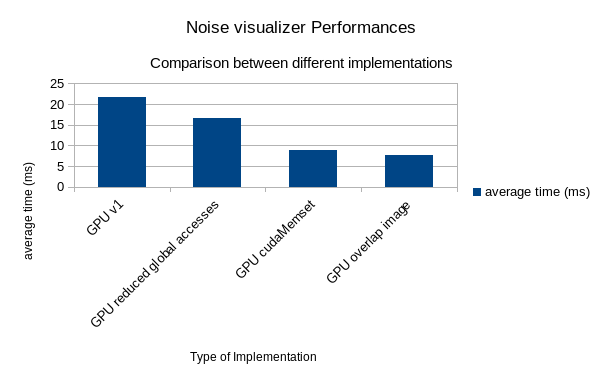
\includegraphics[width=0.6\linewidth]{images/heatmap/noise2}
		\caption{\textit{Comparison between GPU versions for noise visualizer}}
		\label{fig:noise2}
	\end{figure}

	\subsection{Fastest implementation}
	By exploiting the same idea described in the previous paragraph, the algorithm can be even more optimized from the point of view of the execution time. In fact, if instead of taking the two images and compute the difference at pixel level in order to decide if the pixel will be turned red or left as is, the difference computed from the dedicate kernel can be exploited.\newline\newline
	By referring to the Section \ref{sec:streaming}, the output of the kernel that computes the difference pixel by pixel in order to send the difference is stored into the \texttt{h\_diff}. Moreover, an array called \texttt{h\_xs} contains the locations in which the pixels are changed.
	
	The idea is to exploit the \texttt{h\_xs} array in order to turn red the corresponding pixels. Its length is defined by an integer value called \texttt{h\_pos}. 
	Having \texttt{nMaxThreads} threads and \texttt{h\_pos} pixels that must be turned to red, the total threads can work on a portion of \texttt{h\_xs} that is large:
	\[
		maxSect = \frac{nMaxThreads}{h\_xs}
	\]
	This implementation allows to have a huge speedup, since the \texttt{h\_xs} has its corresponding vector already in the Device, called \texttt{d\_xs}; for this reason, it's enough to simply pass the point, without previously perform any memory copy from Device to Host. \newline
	The final CUDA kernel call is like the following C code:
	\begin{lstlisting}[style=CStyle]
// Compute pixel difference		
kernel2<<<1, nMaxThreads, 0>>>(d_current, d_previous, d_diff, max4, d_pos, d_xs);
cudaMemcpyAsync(&pready->h_pos, d_pos, sizeof *d_pos, cudaMemcpyDeviceToHost);
cudaDeviceSynchronize();		

// Comput red map over previous image		
red_black_map_overlap<<<1, nMaxThreads, 0>>>(d_pos, d_xs,
									ceil(pready->h_pos/nMaxThreads), d_previous);\end{lstlisting}
	
	The kernel code will turn the pixels defined in the \texttt{xs} array into red. As said before, each thread will work on a portion of data long \texttt{maxSect} so that the computation load is split. 
	
	The initial problem was to find a way to identify the position of the red component given an arbitrary position of any of the three red, green or blue pixels. The image representation of OpenCV \texttt{Mat} object is slightly misleading; in fact, the blue component is at position 0 while the red one at position 2. So, an image 3x3 pixels is build in the following way:
	\begin{table}[H]
		\centering
		\begin{tabular}{ |c|c|c|c|c|c|c|c|c| } 
			\hline
			B & G & R & B & G & R & B & G & R \\
			\hdashline
			B & G & R & B & G & R & B & G & R \\
			\hdashline
			B & G & R & B & G & R & B & G & R \\
			\hline
		\end{tabular}
		\caption{\textit{Image color component representation, with dimension 3x3}}
	\end{table}
	
	At this point, we know that the red color component is always int the \textit{third} position and so, given an \textit{absolute} index $i$, the corresponding red color component position is identified as:
	\[
		red_{position} = i + (2 - i\%3)
	\]
	
	By applying this idea, the corresponding CUDA kernel is the following one
	\begin{lstlisting}[style=CStyle]
__global__ void red_black_map_overlap(unsigned int *pos, int *xs,
									int maxSect, uint8_t *noise_visualization){
	int x = threadIdx.x + blockDim.x * blockIdx.x;
	int start = x * maxSect;
	int max = start + maxSect;
	
	for (int i = start; i < max && i < *pos; i++) {
		noise_visualization[xs[i] + (2-xs[i]%3)] = 255;
	}
}\end{lstlisting}

	These are the results from \textit{nvprof}, with \texttt{pos} $\simeq 70000$ (number of changed pixels is around 70000):
	\begin{table}[H]
		\centering
		\begin{center}
			\begin{tabular}{ |c|c|c|c|c|c| } 
				\hline
				\textbf{Type} & \textbf{Time} (\%) & \textbf{Avg} & \textbf{Min} & \textbf{Max} & \textbf{Name} \\ 
				\hline
				GPU activities & 7.22 & 915.35us &  624.23us &  6.7692ms & kernel\_red\\
				\hline
			\end{tabular}
		\end{center}
		\label{fig:table_v4_red}
		\caption{\textit{Profiling result for noise visualizer, overwriting the red pixels over the previous frame using \texttt{d\_xs} array. The \textit{[CUDA memcpy DtoH]} and [CUDA memcpy HtoD] are not reported because they can be misleading, since they includes also the cost for the kernel that computes the difference}}
	\end{table}
	
	By considering only the kernel time, the computation time is reduced by 94.5\%, that is pretty impressive.

	\begin{center}
		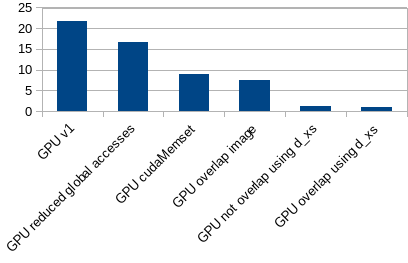
\includegraphics[width=0.6\linewidth]{images/heatmap/noise3}
	\end{center}


	\section{Noise filter}
	The sensor of an digital camera contains a certain number of pixel, used to acquire the image. The settings of a camera allows to adapt the sensor to the external conditions in order to always get the best shot). In a sunny day, a slow  shutter speed, a wide open aperture allows a large number of photons to hit completely the image sensor.
	
	On the other hand, in darker conditions, faster shutter speeds and a closer aperture do not allow enough photons to hit the sensor to generate a suitable voltage to overcome the noise present at the ground. This leads to a low Signal-To-Noise ratio that is directly converted into noise from the internal camera logic. In this case, a correct trim of the of ISO and the shutter aperture time allow to have an image with lower noise; but, in most of the cases, the cheap webcams do not have these advanced configurable feature but perform an auto-adapt procedure.\newline\newline
	This is where the \textit{noise filtering} take a major role for this project. Being the data sent based on the difference with the previous frame, each pixel that is mainly driven by the noise, has higher probability to flip drastically change its value. So, even if the pixel itself does not contains any information, its difference is still sent.
	
	\subsection{Convolution filters}
	Convolution filters are used to perform some perturbation over an image in order to obtain some enhancement. They are based on a \textit{kernel}, a convolution matrix, that is used to perform the convolution between the image and the kernel itself, in the following way:
	
	\begin{align*}
		g(x,y) = \sum_{u = \frac{-k}{2}}^{\frac{k}{2}} \sum_{v = \frac{-k}{2}}^{\frac{k}{2}} K[u,v] \cdot I(x-u, y-u)
	\end{align*}
	
	Where $K$ is the kernel and $I$ is the original image; $g$ will be the perturbed resulting image. Depending on the type of selected kernel, the image will be modified in a different way. By defining the size of the kernel as $3\cdot 3$, the identity is the following:
	\begin{center}
		$
		K = \begin{bmatrix}
			0 & 0 & 0\\
			0 & 1 & 0\\
			0 & 0 & 0
		\end{bmatrix}
		$
	\end{center}
	In this way, the original image is not modified; let's check it:
	\begin{align*}
		 I * K & =\left({\begin{bmatrix}a&b&c\\d&e&f\\g&h&i\end{bmatrix}}*{\begin{bmatrix}0&0&0\\0&1&0\\0&0&0\end{bmatrix}}\right) = \\
			&=(i\cdot 0)+(h\cdot 0)+(g\cdot 0)+(f\cdot 0)+(e\cdot 1)+(d\cdot 0)+(c\cdot 0)+(b\cdot 0)+(a\cdot 0)\\
			&= e
	\end{align*}

	
	\subsection{Mean filter}
	The idea of the Mean filter, also called \textit{blur box}, is to set the kernel with the elements that have all the same weight but normalized, like in the following 3x3 convolution matrix:
	\begin{center}
		$
		K = \frac{1}{9}\begin{bmatrix}
			1 & 1 & 1\\
			1 & 1 & 1\\
			1 & 1 & 1
		\end{bmatrix} = \begin{bmatrix}
		0.11 & 0.11 & 0.11\\
		0.11 & 0.11 & 0.11\\
		0.11 & 0.11 & 0.11
	\end{bmatrix}
		$
	\end{center}
	It can be simple computed in the following way, assuming the kernel is on $KxK$:
	\begin{lstlisting}[style=CStyle]
float* computeMeanKernel(int K){
	double sum = 0;
	float* k = (float*)malloc(K*K*sizeof(float));
	for (int i = 0; i < K; i++){
		for (int j = 0; j < K; j++){
			k[i*K+j] = 1.0/(K*K);
		}
	}
	
	return k;
}\end{lstlisting}	
	In this way, the image is basically blurred due to the fact that the pixel at $i$ position is based now also on the values of the surrounding 8 pixels.

	\begin{figure}[H]
		\centering
		\begin{minipage}[b]{0.45\textwidth}
			\centering
			
\includegraphics[width=0.32\textwidth]{images/heatmap/scoiattolo1.png}
			\caption{\textit{Original}}
		\end{minipage}
		\hfill
		\begin{minipage}[b]{0.45\textwidth}
			\centering
			
\includegraphics[width=0.32\textwidth]{images/heatmap/scoiattolo1_blur.png}
			\caption{\textit{Mean filtering 3x3}}
		\end{minipage}
	\end{figure}

	This solution can be exploited in order to make the pixels that suffers from the noise problem more smooth with the respect to the neighbors ones. In this way, even if the two consecutive frames are not exactly the same, the difference among the single pixels will be lower, resorting to a lower data sent over the socket. Let's take for simplicity two frames that are in gray scale, between 0 and 255, that are describes as two 3x3 matrices.
	\begin{center}
		$
		A = \frac{1}{9}\begin{bmatrix}
		120 & 131 & 112\\
			112 & 101 & 82\\
			44 & 106 & 65
		\end{bmatrix}
	\quad\quad B = \begin{bmatrix}
			120 & 139 & 90\\
			99 & 126 & 106\\
			46 & 75 & 88
		\end{bmatrix}
		$
	\end{center}
	If we simply compute the difference, and we set the threshold to 20, by computing the difference location by location, 5 pixels must be sent as difference. If we apply now the kernel to both the two frames, in order to simulate the behaviour of the algorithm, the two resulting matrices are the following:
	\begin{center}
		$
		A = \frac{1}{9}\begin{bmatrix}
			51 & 73 & 47\\
			68 & 96 & 66\\
			40 & 56 & 39
		\end{bmatrix}
		\quad\quad B = \begin{bmatrix}
			53 & 75 & 51\\
			67 & 98 & 69\\
			38 & 60 & 43
		\end{bmatrix}
		$
	\end{center}
	As you can see now, no pixels need to be sent. This is a huge improvement, since we have saved 100\% of the bandwidth if we neglect the overhead to transmit the information that no pixels have changed. Even if this seems an optimal solution, it has one major drawback. The image will became distorted from the details point of view. In fact, a trade-off between image quality and saved bandwidth must be selected.


	\subsection{Gaussian filter}
	The second type of filter that has been selected to reduce the noise, is the \textit{Gaussian filter}, that allows to reach a similar result with the respect to the Mean one. The idea is always to distorce the image to reduce the noise and make the difference among pixels lower. The matrix of a 3x3 Gaussian filter is the following:
		\begin{center}
		$
		K = \frac{1}{16}\begin{bmatrix}
			1 & 2 & 1\\
			2 & 4 & 2\\
			1 & 2 & 1
		\end{bmatrix}
		$
	\end{center}
	It can be computed using the following formula:
	\begin{align*}
		K(x,y) = \frac{1}{2 \cdot \pi \cdot \sigma^2}\cdot e^{-\frac{x^2 + y^2}{2 \sigma^2}}
	\end{align*}
	It is called Gaussian filter because of its shape, corresponds to a Gaussian function. A filter of this type requires $6 \sigma - 1$ values (to make it sure it's odd), so that for a $\sigma$ of 3 the kernel must be 17 elements long. The $\sigma$ value if given is pixels. If we use a square kernel its size can be simply computed as:
	\[
		side_{lenght} = \sqrt{6 \cdot \sigma - 1}
	\]
	Where $side_{lenght}$ is one of the length of the matrix that composes the kernel. A visual example representation is available in the following image.
	\begin{center}
		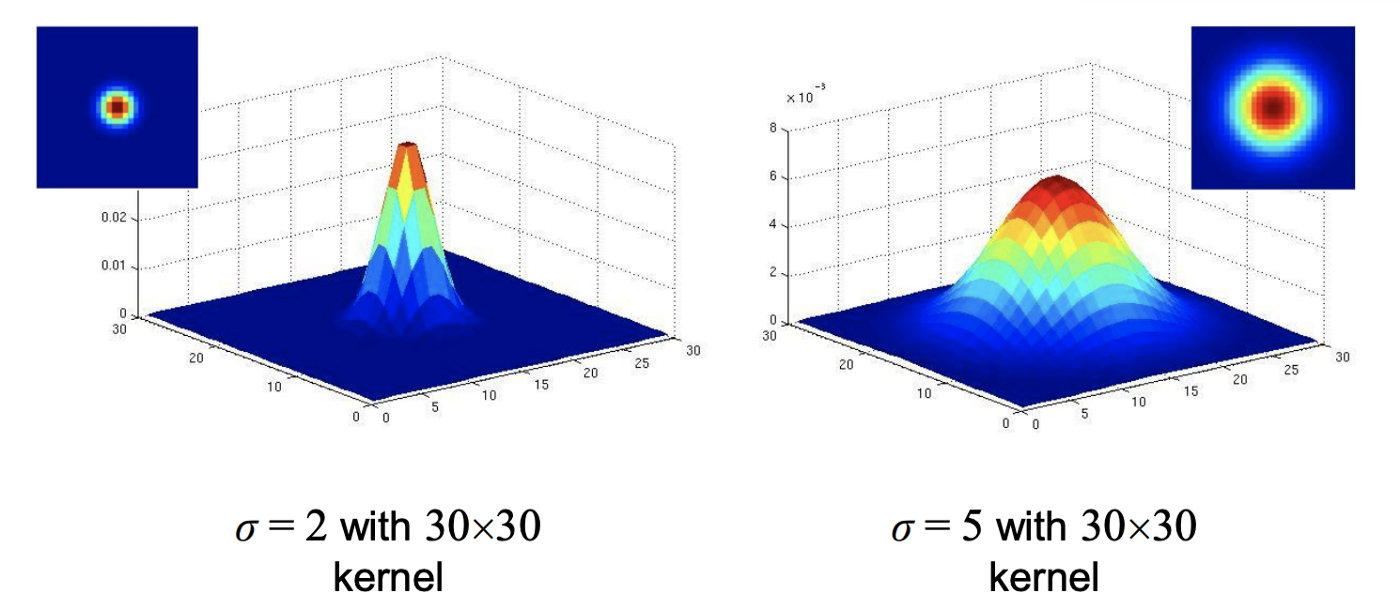
\includegraphics[width=0.45\linewidth]{images/heatmap/sigma_representation}
	\end{center}
	Gaussian filter weights pixels into a bell-shape curve around the central pixel. This means that the farther the pixel from the center, the lower the weight. On the other hand the Mean filter is just an average between the center and the neighboring pixels. This means that that for all the pixels, equal weights are assigned, regardless the distance from the center.
		\begin{figure}[H]
		\centering
		\begin{minipage}[b]{0.45\textwidth}
			\centering
			
\includegraphics[width=0.32\textwidth]{images/heatmap/scoiattolo1.png}
			\caption{\textit{Original}}
		\end{minipage}
		\hfill
		\begin{minipage}[b]{0.45\textwidth}
			\centering
			
\includegraphics[width=0.32\textwidth]{images/heatmap/scoiattolo1_gaussian.png}
			\caption{\textit{Gaussian filter 3x3}}
		\end{minipage}
	\end{figure}

	The C code, that give $\sigma$, computes the entire convolution matrix is the following:
\begin{lstlisting}[style=CStyle]
float* computeGaussianKernel(float s, int K){
	float sum = 0;
	float* k = (float*)malloc(K*K*sizeof(float));
	for (int i = 0; i < K; i++){
		for (int j = 0; j < K; j++){
			double x = i - (K - 1) / 2.0;
			double y = j - (K - 1) / 2.0;
			k[i*K+j] = (1.0/(2.0*M_PI*s*s)) * exp(-((x*x + y*y)/(2.0*s*s)));
			sum += k[i*K+j];
		}
	}
	for (int i = 0; i < K; i++) {
		for (int j = 0; j < K; j++) {
			k[i*K+j] /= sum;
		}
	}
	
	return k;
}\end{lstlisting}	

	\subsection{Tiled CUDA 2D implementation}
	In order to test the effectiveness of the algorithm and if it is suitable for this project, a configurable implementation has been developed in CUDA. In order to have all the same test environment, two sequential frames have been taken from the webcam in a semi dark environment with a person in the center. 
	
	\begin{figure}[H]
		\centering
		\begin{minipage}[b]{0.45\textwidth}
			\centering
			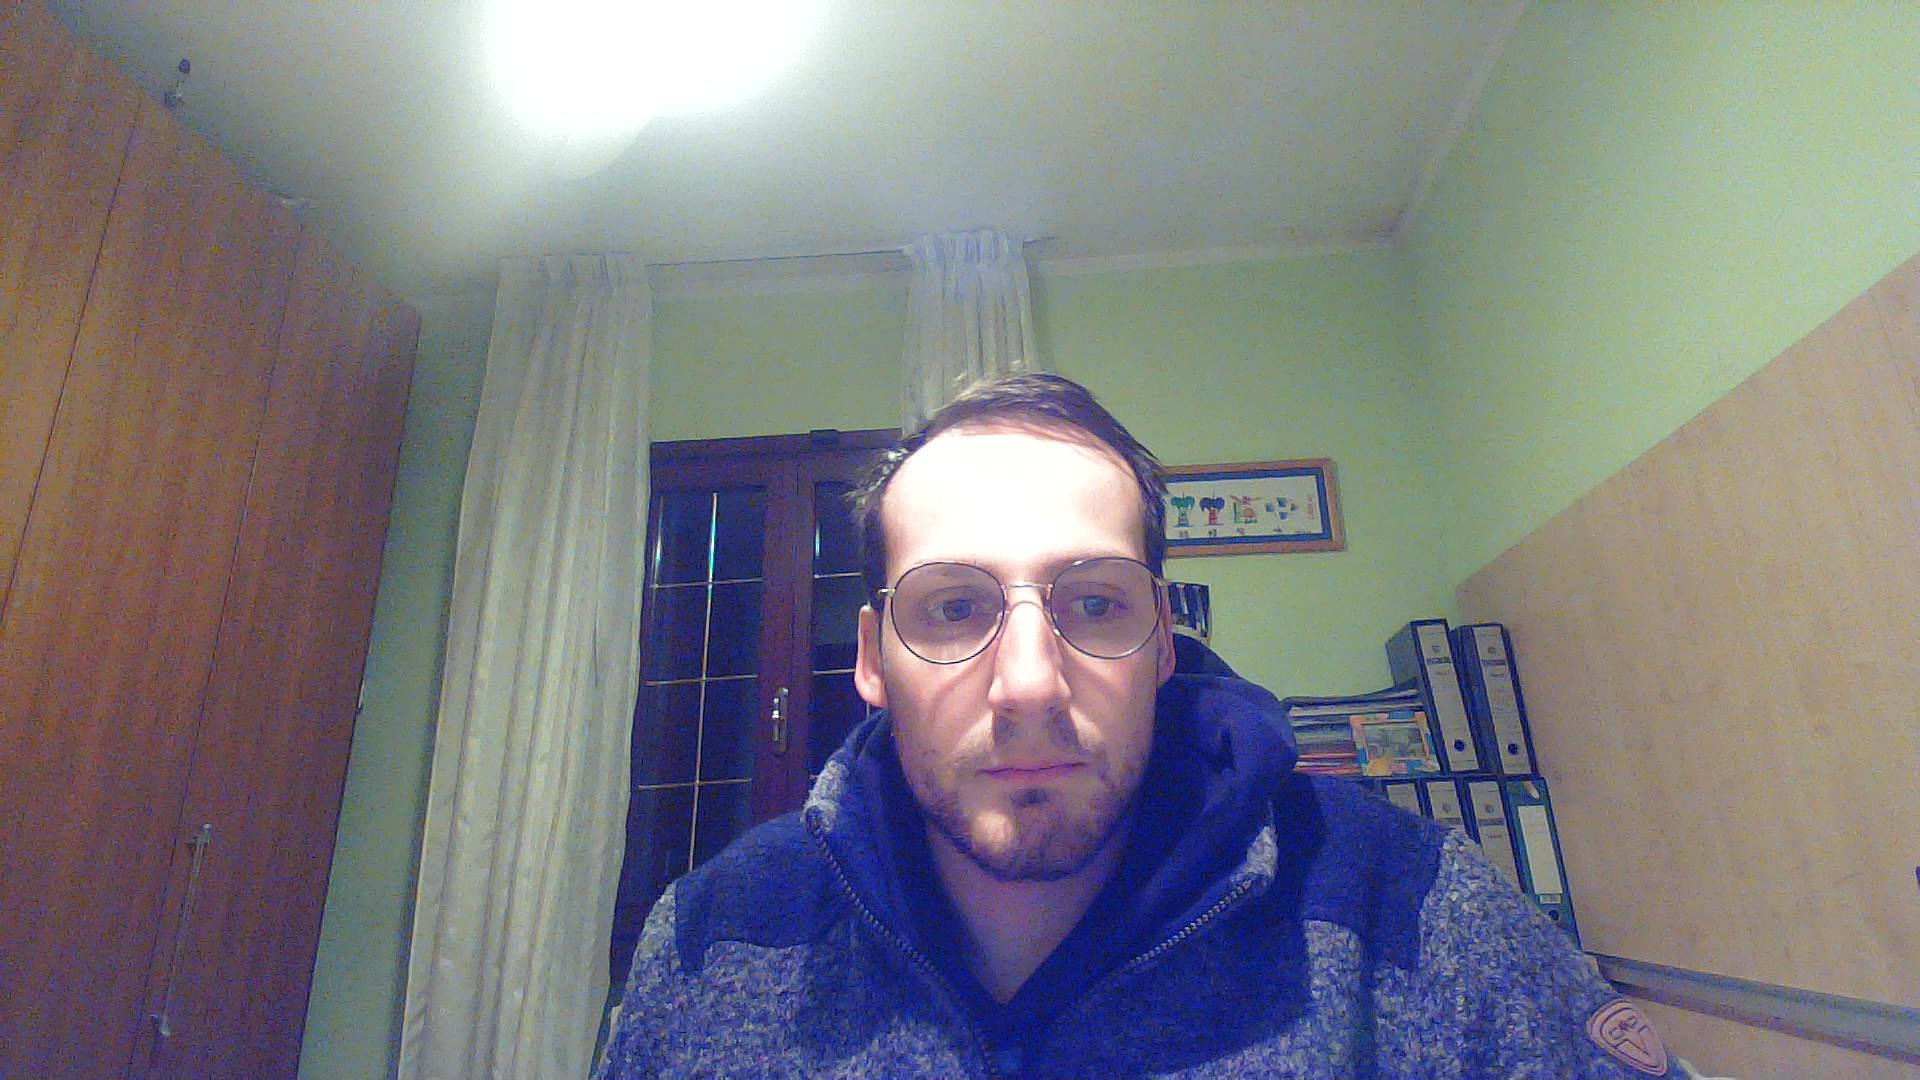
\includegraphics[width=0.85\textwidth]{images/heatmap/f1.jpg}
			\caption{\textit{First frame}}
		\end{minipage}
		\hfill
		\begin{minipage}[b]{0.45\textwidth}
			\centering
			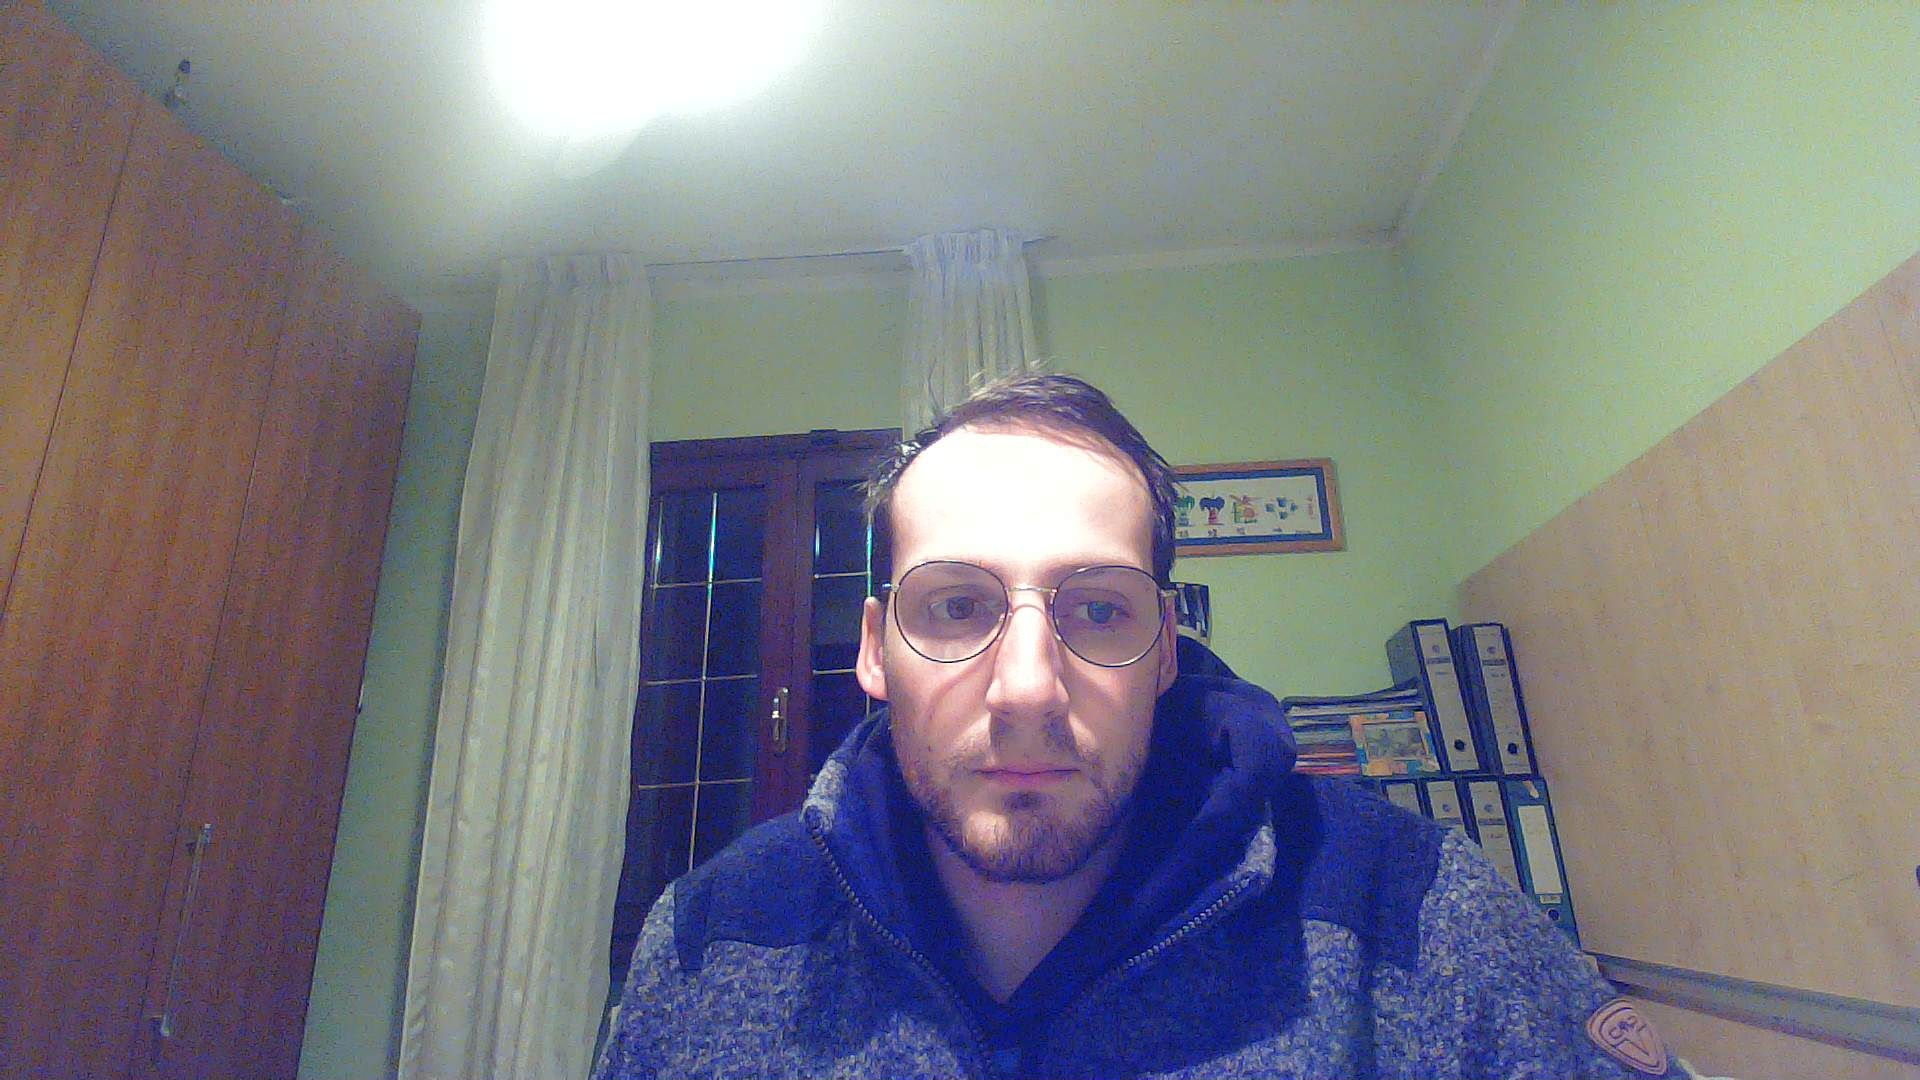
\includegraphics[width=0.85\textwidth]{images/heatmap/f2.jpg}
			\caption{\textit{Second frame}}
		\end{minipage}
	\end{figure}
	As you can see, the two images are pretty similar in term of content; a trained eye can see that the head of the second frame is slightly tilted to the right with the respect to the previous one. The idea is to run now the \textit{noise visualizer}, refer to Section \ref{sec:noise_visualizer}, on these two frames and understand where the noise is located.
	\begin{figure}[H]
		\centering
		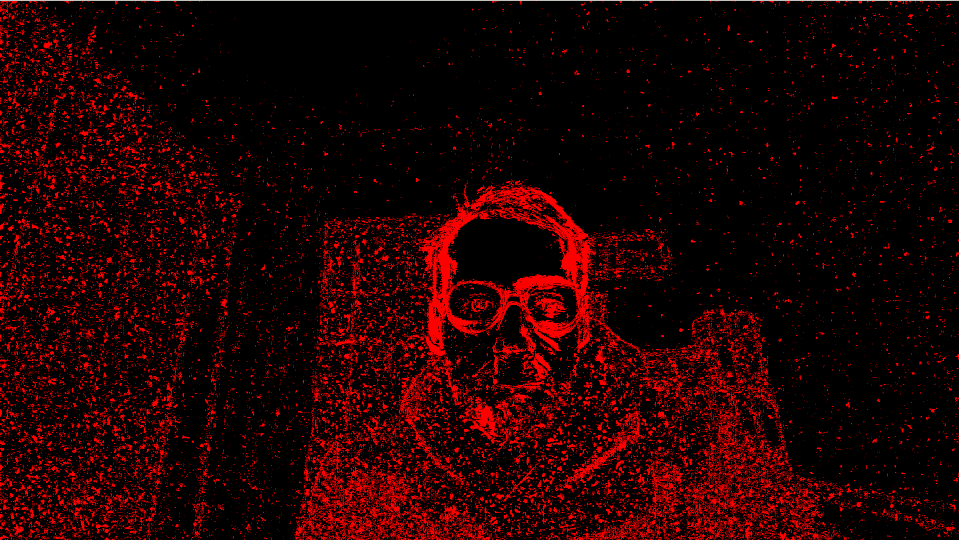
\includegraphics[width=0.35\linewidth]{images/heatmap/noise_visual}
		\caption{\textit{Red-black representation of the noise}}
		\label{fig:noisevisual}
	\end{figure}
	The noise, is the one in the background that do not contribute in any way to the video flow. In fact, even if it is fixed, it is sent anyway via the socket, increasing the used bandwidth. The CUDA implementation is based on the 2D tiled version but includes the management for all three color components.\newline\newline
	The entire algorithm is based on the usage of the shared memory and the synchronization among the thread. The idea is to make each thread work on single pixel and apply the kernel, by using the portion of the image that is in the shared memory, called \textit{tile}. 

	The kernel implementation is composed of multiple parts:
	\begin{enumerate}
		\itemsep0sp
		\item \textbf{Shared memory initialization and boundary condition management}:
		As introduced before, each thread, identified by its $ty$ and $tx$ coordinates should work on a precise pixels, identified as:
		\begin{lstlisting}[style=CStyle]
__shared__ int N_ds[BLOCK_SIZE][BLOCK_SIZE*3];

x = threadIdx.x + blockIdx.x*TILE_SIZE - K/2;
y = threadIdx.y + blockIdx.y*TILE_SIZE - K/2; \end{lstlisting}
	In fact, the idea is to create a block of threads that corresponds to \texttt{BLOCK\_SIZE}*\texttt{BLOCK\_SIZE} as dimension, so that each one of the loads into the shared memory the value of its pixel (the multiplication by 3 in the kernel implies that each threads read all three color components). The following code, instead, includes also the write into the shared memory.
		
		\begin{lstlisting}[style=CStyle]
int tx = threadIdx.x;   //W
int ty = threadIdx.y;   //H
int row_o = blockIdx.y*TILE_SIZE + ty;
int col_o = blockIdx.x*TILE_SIZE + tx;
int row_i = row_o - K/2;
int col_i = col_o - K/2;

if(row_i >= 0 && row_i < H && col_i >= 0 && col_i < W){
	N_ds[ty][tx*3] = image[row_i*W*3+ col_i * C];
	N_ds[ty][tx*3+1] = image[row_i*W*3+ col_i*3 + 1 ];
	N_ds[ty][tx*3+2] = image[row_i*W*3+ col_i*3 + 2 ];
} else {
	N_ds[ty][tx*3] = 0;
	N_ds[ty][tx*3+1] = 0;
	N_ds[ty][tx*3+1] = 0;
}	\end{lstlisting}
	The value \texttt{TILE\_SIZE} defines the dimension of the tile, in which each the kernel is applied. The problem is that, the first pixel (position [0,0]) in the image, if the kernel has a dimension of 3x3, need to access also the location [-1,-1], [-1, 0], [-1, 1], [0, -1], [1, -1]. In this case, they are not available. This is the reason of the presence of the if condition, that sets 0 at these locations in the shared memory by ``shifting" the indexes by $K/2$. The problem is shown in the below picture:
		\begin{figure}[H]
			\centering
			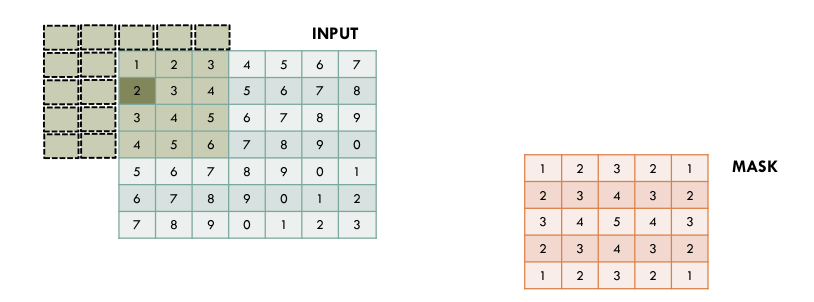
\includegraphics[width=0.5\linewidth]{images/heatmap/kernel_and_mask}
			\caption{\textit{Boundary conditions among the image border}}
			\label{fig:kernelandmask}
		\end{figure}
	In this way, all the pixels needed to process a tile of \texttt{TILE\_SIZE}x\texttt{TILE\_SIZE} dimension, are loaded into the \texttt{N\_ds} shared memory that is large \texttt{BLOCK\_SIZE}*\texttt{BLOCK\_SIZE*3} in order to contains also the values at the boundary of the tile.
		\item \textbf{Filter application}:
		Foreach element in the tile and for all three color components, the kernel is computed using the shared memory. 
	\end{enumerate}
	 


	The entire kernel is the following:

\begin{lstlisting}[style=CStyle]
__constant__ float dev_k[K*K];

__global__ void convolution_kernel(uint8_t *image, uint8_t *R)
{
	__shared__ int N_ds[BLOCK_SIZE][BLOCK_SIZE*3];
	
	int tx = threadIdx.x;   //W
	int ty = threadIdx.y;   //H
	int row_o = blockIdx.y*TILE_SIZE + ty;
	int col_o = blockIdx.x*TILE_SIZE + tx;
	int row_i = row_o - K/2;
	int col_i = col_o - K/2;
	
	// Management of the boudary conditions
	if(row_i >= 0 && row_i < H && col_i >= 0 && col_i < W){
		N_ds[ty][tx*3] = image[row_i*W*3+ col_i * C];
		N_ds[ty][tx*3+1] = image[row_i*W*3+ col_i*3 + 1 ];
		N_ds[ty][tx*3+2] = image[row_i*W*3+ col_i*3 + 2 ];
	} else {
		N_ds[ty][tx*3] = 0;
		N_ds[ty][tx*3+1] = 0;
		N_ds[ty][tx*3+1] = 0;
	}
	
    __syncthreads();

	if(row_o < H && col_o < W){
		float outputR = 0.0;
		float outputG = 0.0;
		float outputB = 0.0;
		if(ty < TILE_SIZE && tx < TILE_SIZE){
			for(int i = 0; i < K; i++)
			for(int j = 0; j < K; j++){
				outputR += dev_k[i*K+j] * N_ds[i+ty][(j+tx)*3];
				outputG += dev_k[i*K+j] * N_ds[i+ty][(j+tx)*3 + 1];
				outputB += dev_k[i*K+j] * N_ds[i+ty][(j+tx)*3 +2];
			}
			
			R[row_o*W*3 + col_o*3] = outputR;
			R[row_o*W*3 + col_o*3 + 1] = outputG;
			R[row_o*W*3 + col_o*3 + 2] = outputB;
		}
	}
}\end{lstlisting}

	The kernel call needs to work on an image of 1920*1080*3 elements divided into square tiles of \texttt{TILE\_SIZE}x\texttt{TILE\_SIZE} dimensions. Since the tile needs also the surrounding element to compute the kernel, the block size is composed of \texttt{BLOCK\_SIZE}x\texttt{BLOCK\_SIZE} elements, where:
	\[
		BLOCK\_SIZE = TILE\_SIZE + K - 1
	\]
	
	The grid instead, is configured to generate as many tile as needed from the image. In this case, a grid of \texttt{W/TILE\_SIZE}x\texttt{H/TILE\_SIZE} is enough (need to be rounded to the upper value).
	This is the complete kernel call
\begin{lstlisting}[style=CStyle]
dim3 blockSize, gridSize;
blockSize.x = BLOCK_SIZE, blockSize.y = BLOCK_SIZE, blockSize.z = 1;
gridSize.x = ceil((float)W/TILE_SIZE),
gridSize.y = ceil((float)H/TILE_SIZE),
gridSize.z = 1;

// Kernel call
convolution_kernel<<<gridSize, blockSize>>>(d_current, d_current_filtered);
\end{lstlisting}

	 This solution includes already optimal solution in order to increase the performance and reduce at minimum the overhead introduced by the computation of the filter. In fact, by having defined how convolution if performed, it can be simple called, after have set the kernel in the constant memory.
	 
	 Having defined the kernel, that once computed is fixed for the entire program execution, allows to not cope with the cache coherence management, allowing data to be aggressively cached in the L1 cache (the nearest to the SM).
	
	Moreover, access to the memory has been optimized by resorting to the usage of the shared memory. Since the larger the dimension of the tile, the higher the ration between the manipulated pixels and the memory accesses, an optimal solution is to increase as much as possible the tile size. The limit is the shared memory, that is limited. \newline\newline
	The execution of the kernel is directly proportional to the size of the tile and the kernel dimension; the code shown before has been run for multiple sessions in order to be able to plot the kernel time for multiple convolution matrix and multiple tile size.

	\begin{figure}[H]
		\centering
		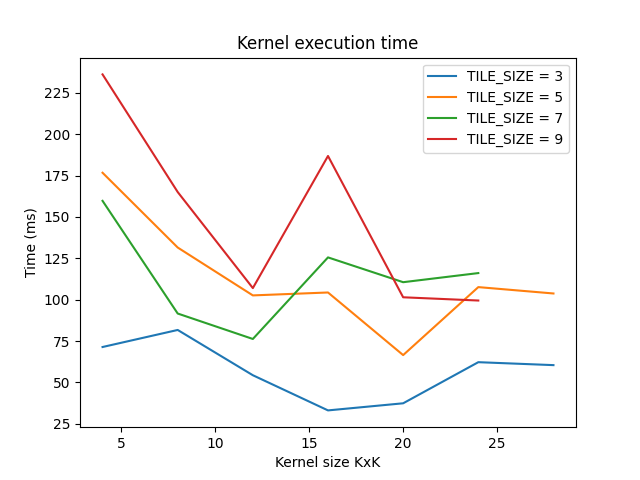
\includegraphics[width=0.42\linewidth]{images/heatmap/kernel_time_noise_2.png}
		\caption{\textit{Kernel execution time from profiler}}
		\label{fig:noise_kernel_time}
	\end{figure}

	Both the Gaussian and the Mean filters have been run over the two frames used as test dataset, the results are available at Table \ref{fig:filter_exe}. The number of pixels changed, if no filter is applied, is 369350, that is 5.93\% of the whole image.
	\begin{figure}[H]
		\centering
		\begin{center}
			\begin{tabular}{ |c|c|c| } 
				\hline
				\textbf{Filter Type} & \textbf{Kernel size}  & \textbf{Total saved pixels}  (\%) \\ 
				\hline
				Mean & 3 & 3.37\\
					 & 5 & 2.31\\
					 & 7 & 1.66\\
					 & 9 & 1.24\\
					 \hline
				Gaussian & 3 ($\sigma=1$) & 3.58\\ 
						& 4 ($\sigma=2$) & 2.87\\ 
						& 5 ($\sigma=3$) & 2.37\\ 
						& 6 ($\sigma=5$) & 1.98\\ 
						& 7 ($\sigma=8$) & 1.66\\ 
				\hline
			\end{tabular}
		\end{center}
		\caption{\textit{Results of both Gaussian and Mean filter, with different kernel size}}
		\label{fig:filter_exe}
	\end{figure}

	\begin{figure}[H]
		\centering
		\begin{subfigure}{0.2\textwidth}
			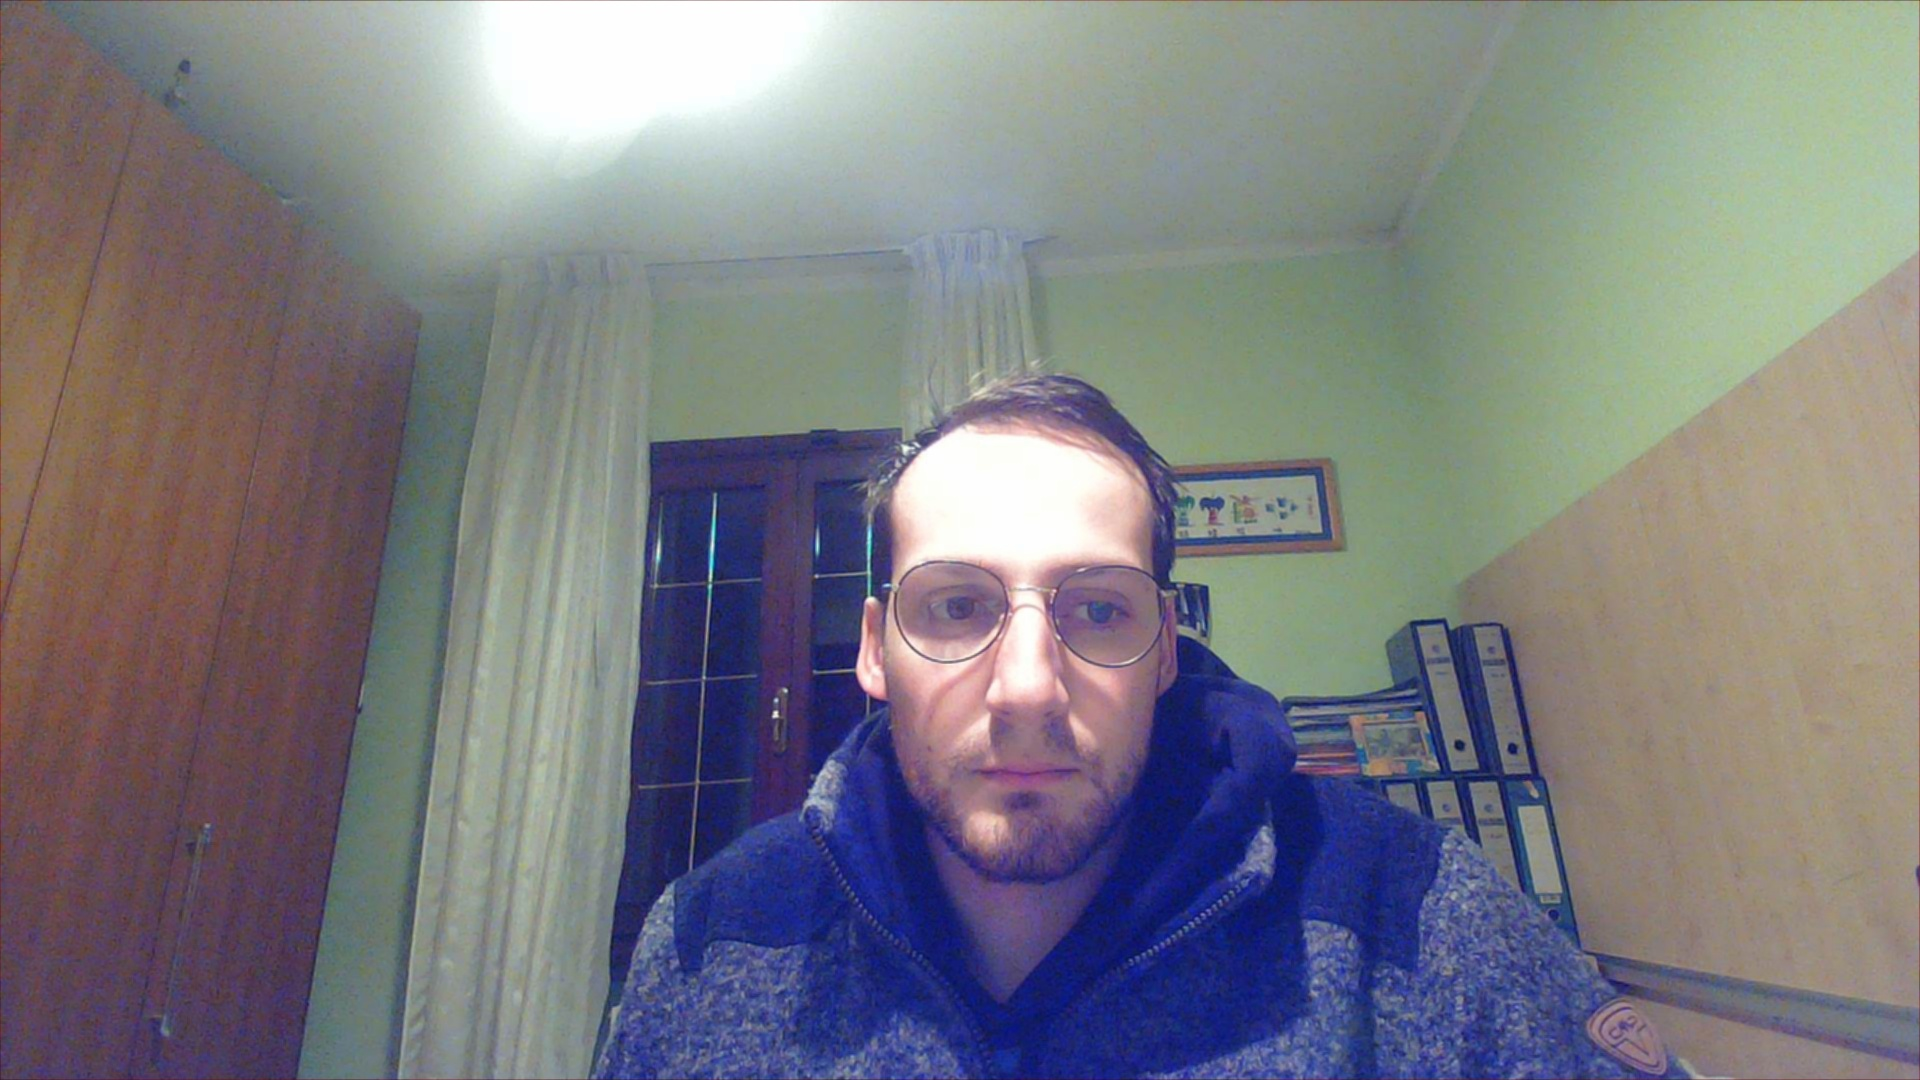
\includegraphics[width=\linewidth]{images/heatmap/img_mean/img_man3.jpg}
		\end{subfigure}%
		\begin{subfigure}{0.2\textwidth}
			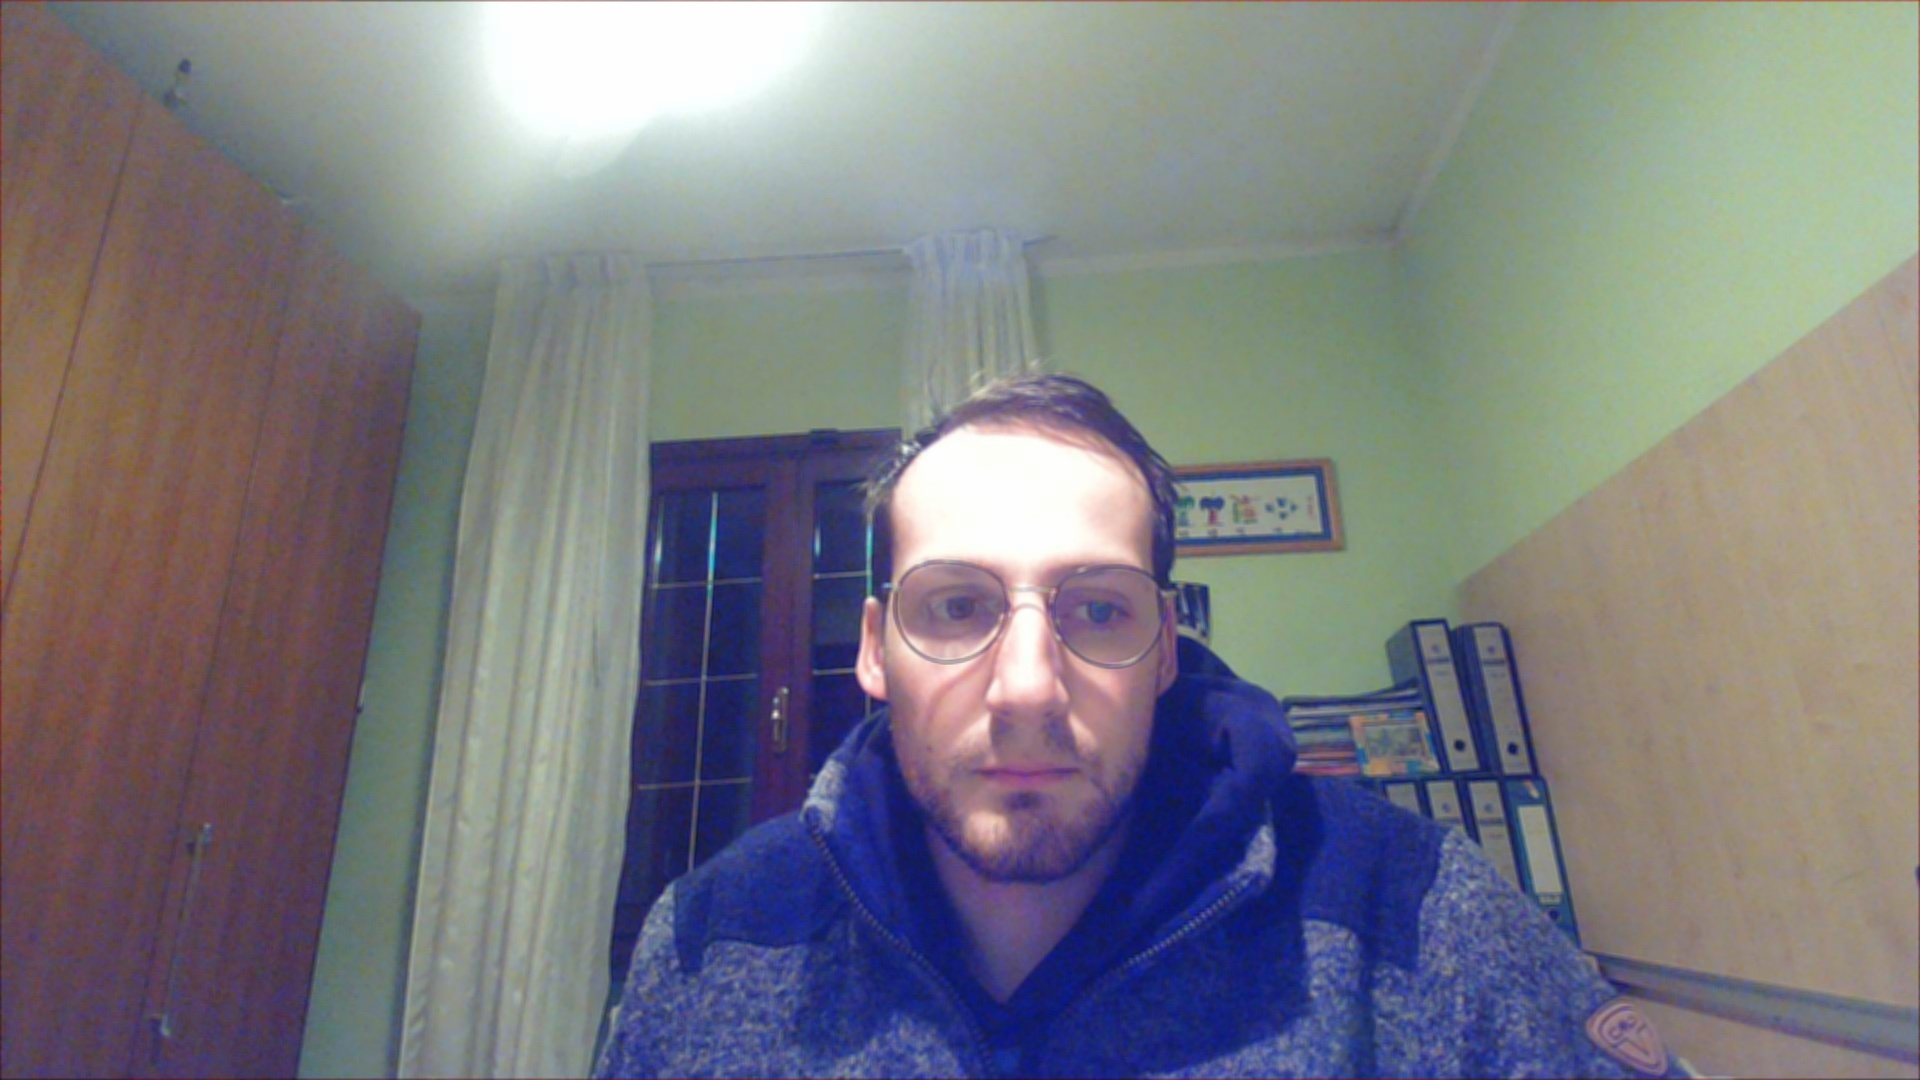
\includegraphics[width=\linewidth]{images/heatmap/img_mean/img_man5.jpg}
		\end{subfigure}%
		\begin{subfigure}{0.2\textwidth}
			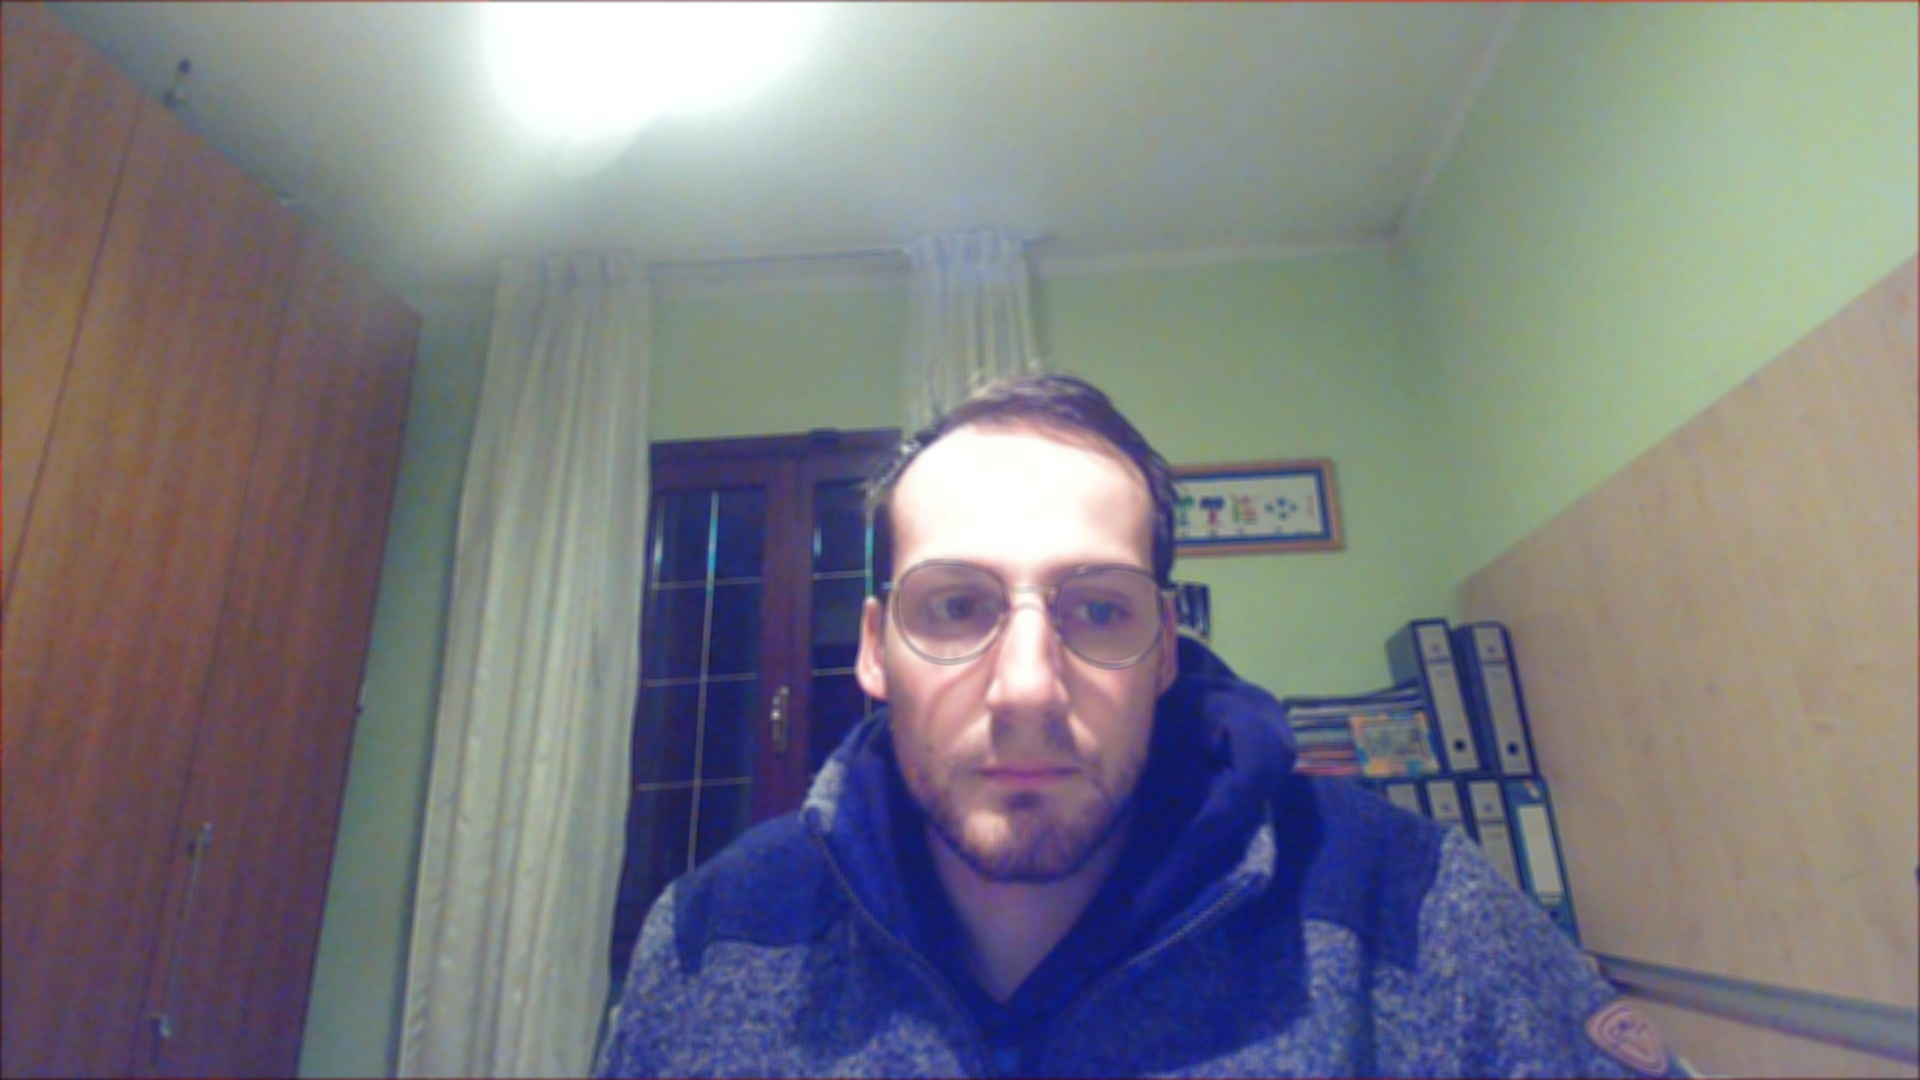
\includegraphics[width=\linewidth]{images/heatmap/img_mean/img_man7.jpg}
		\end{subfigure}%
		\begin{subfigure}{0.2\textwidth}
			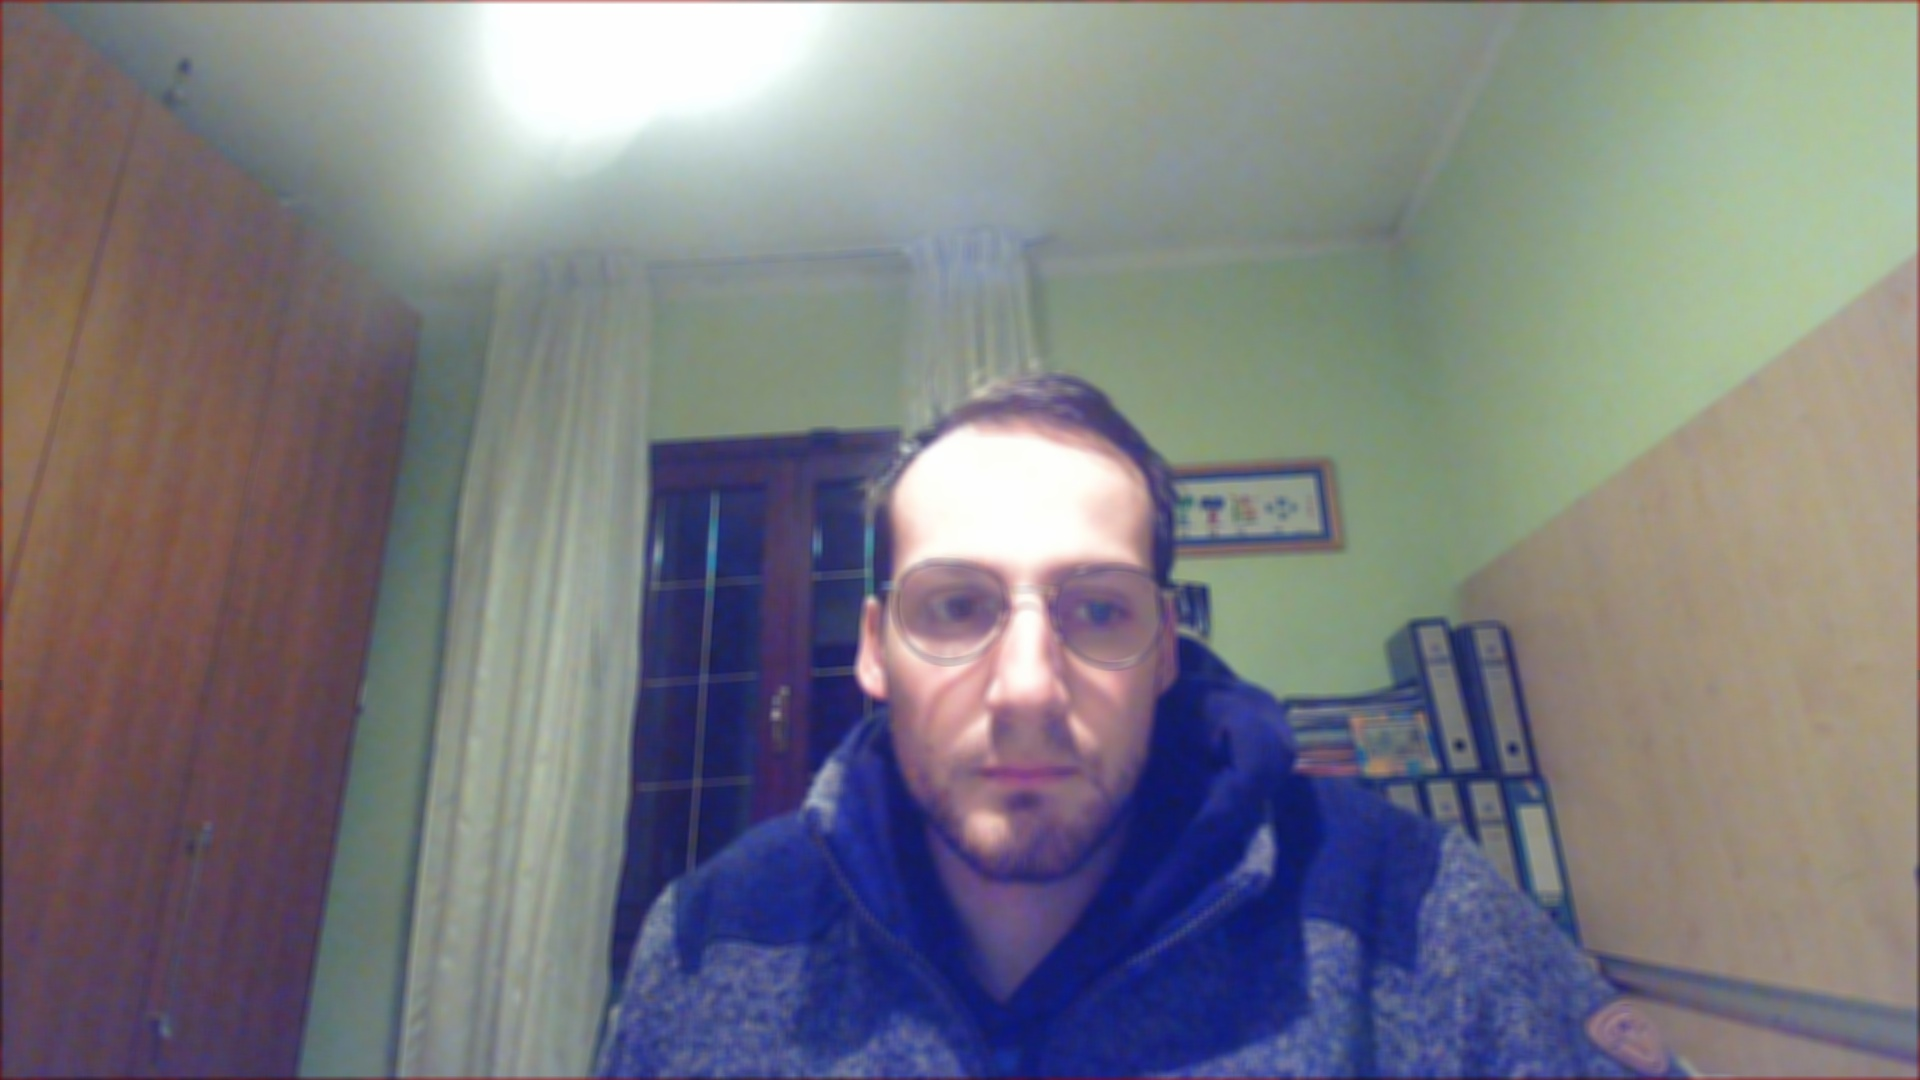
\includegraphics[width=\linewidth]{images/heatmap/img_mean/img_man9.jpg}
		\end{subfigure}
	
		\begin{subfigure}{0.2\textwidth}
			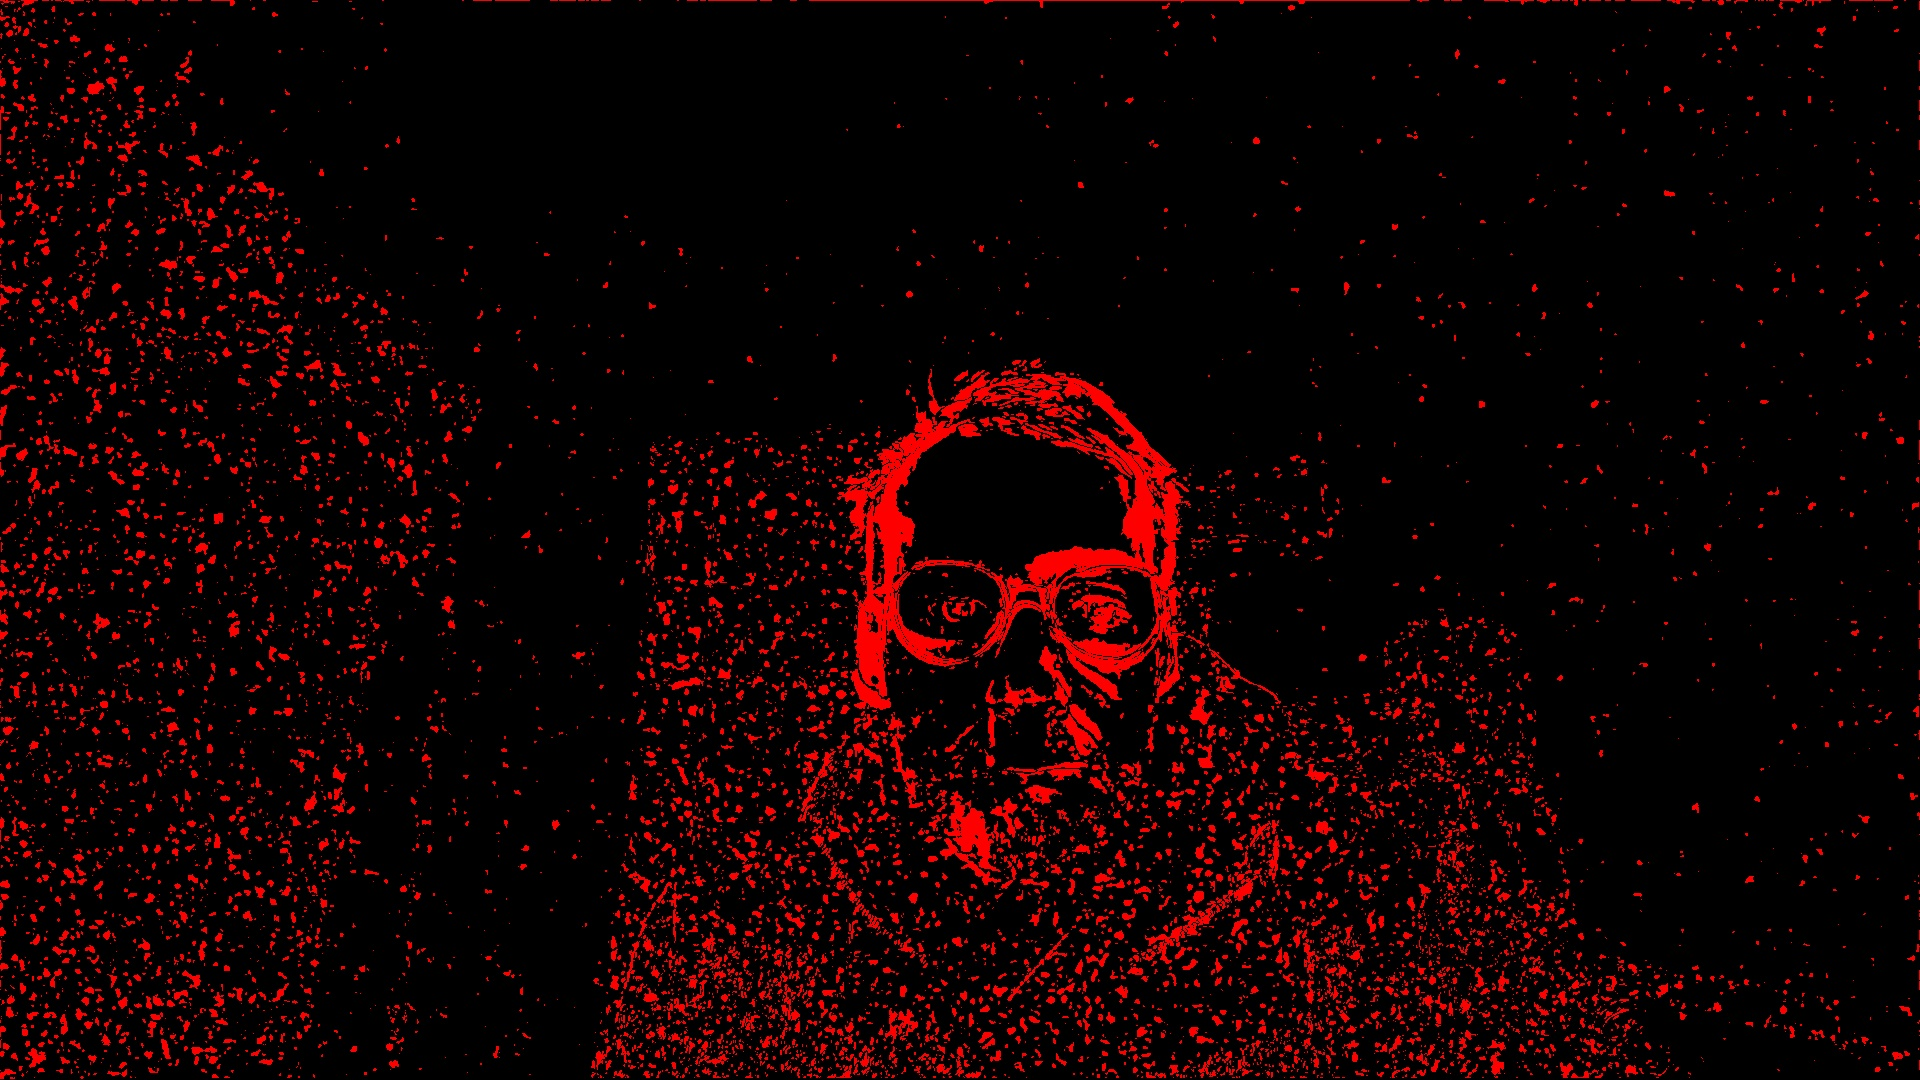
\includegraphics[width=\linewidth]{images/heatmap/img_mean/img_man_red3.jpg}
			\caption{$K=3$}
		\end{subfigure}%
		\begin{subfigure}{0.2\textwidth}
			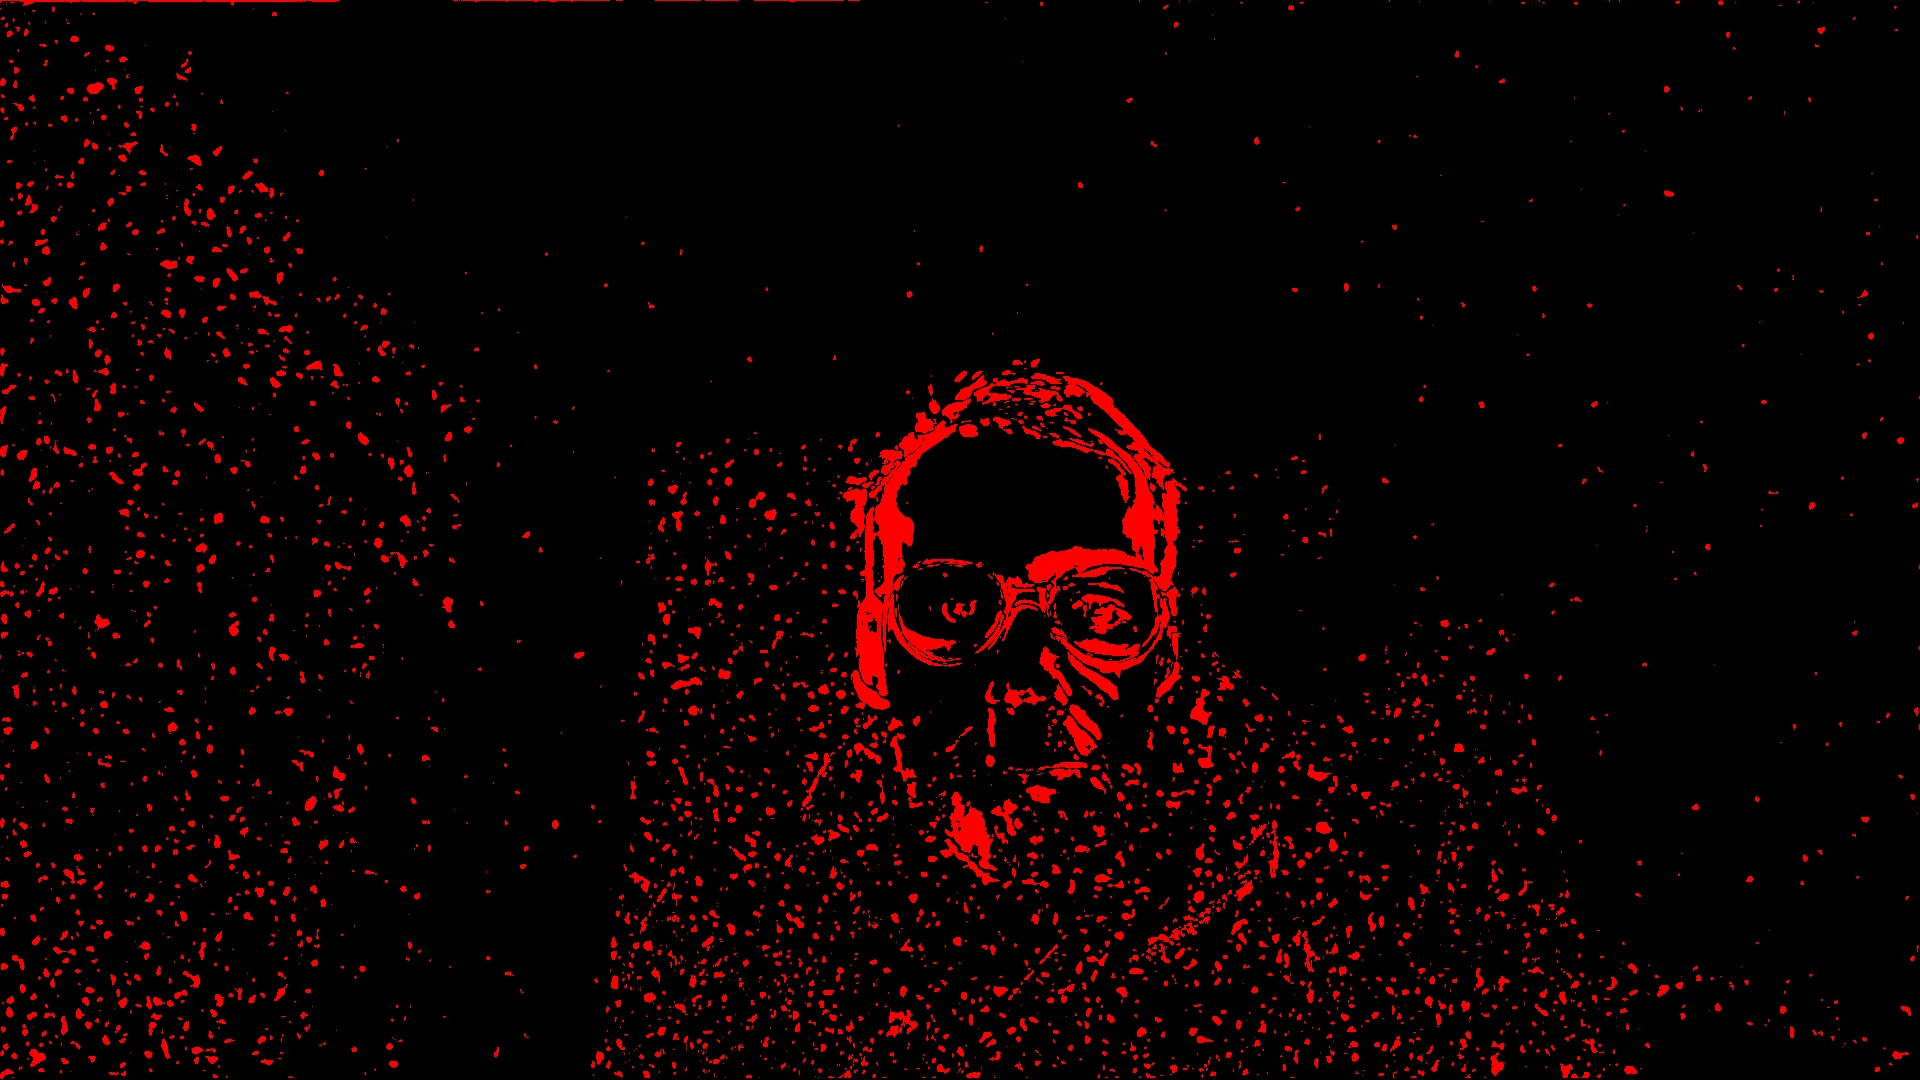
\includegraphics[width=\linewidth]{images/heatmap/img_mean/img_man_red5.jpg}
			\caption{$K=5$}
		\end{subfigure}%
		\begin{subfigure}{0.2\textwidth}
			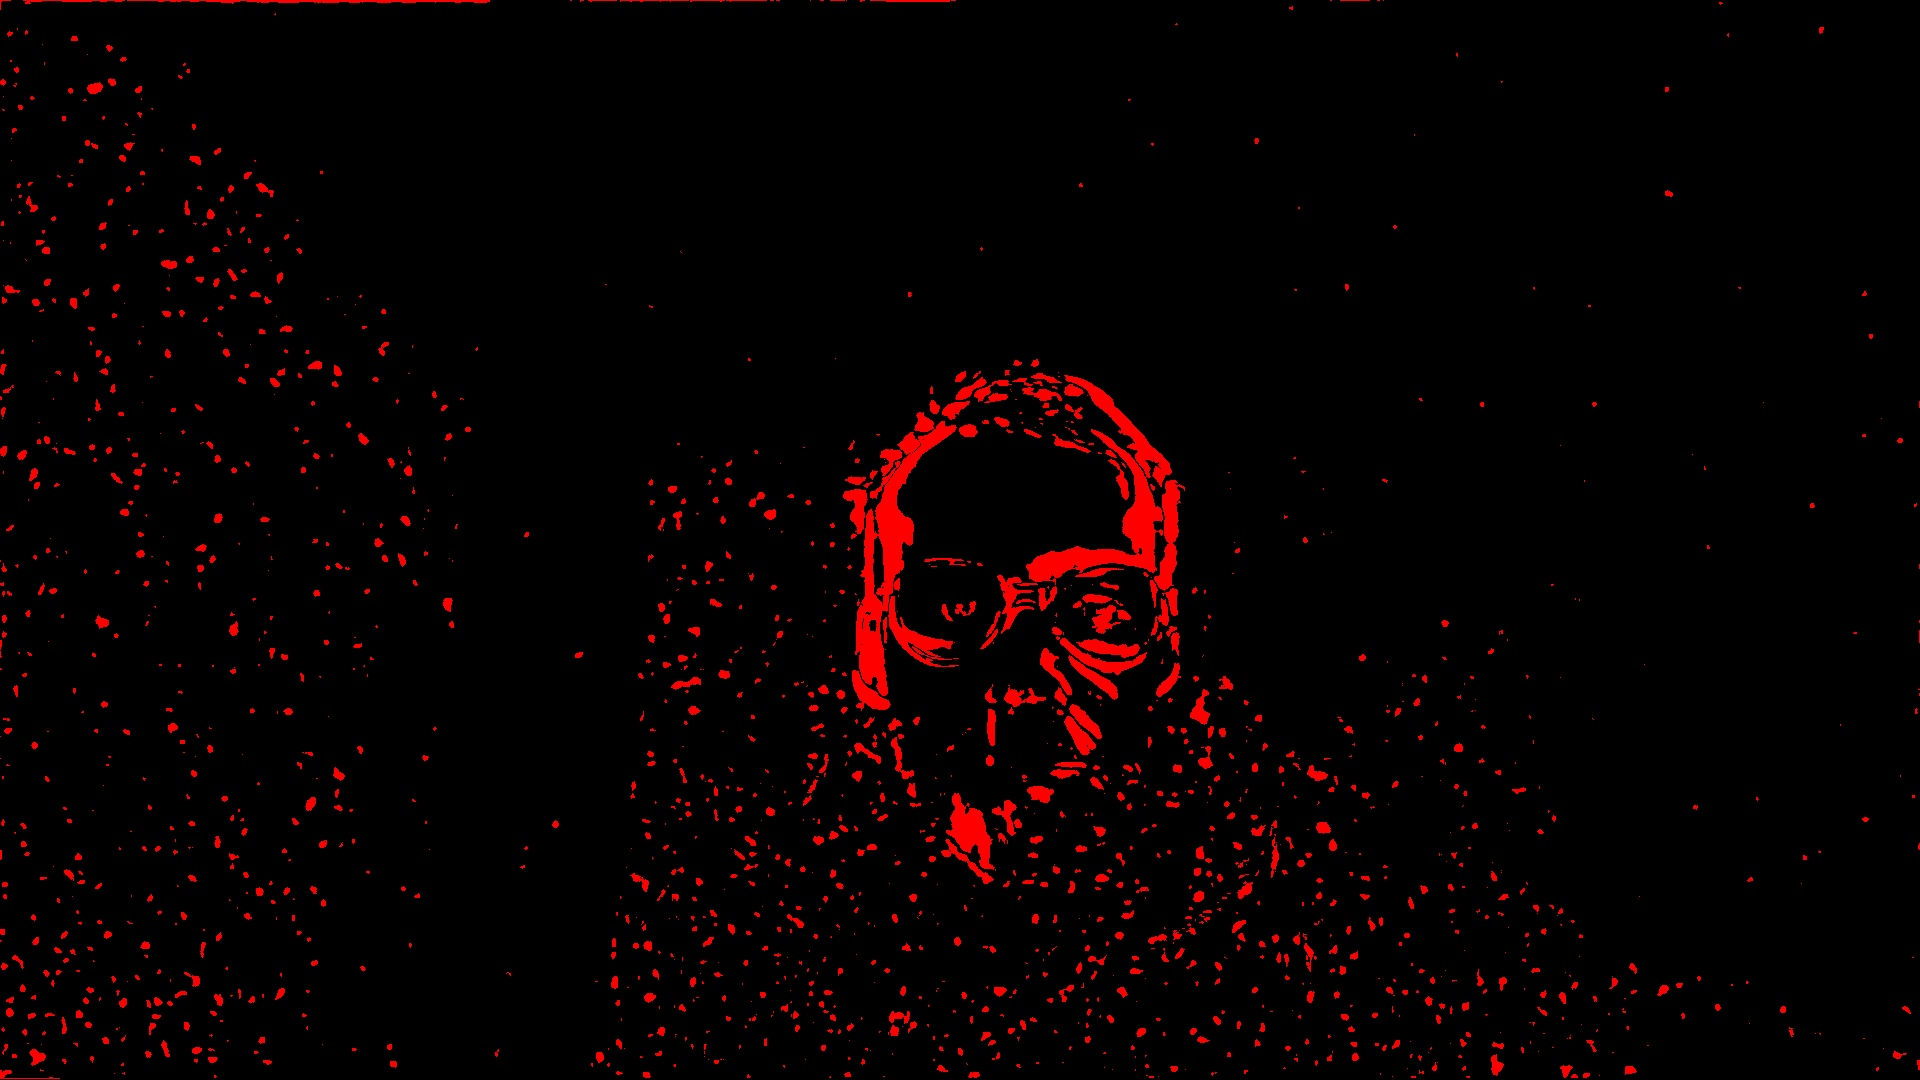
\includegraphics[width=\linewidth]{images/heatmap/img_mean/img_man_red7.jpg}
			\caption{$K=7$}
		\end{subfigure}%
		\begin{subfigure}{0.2\textwidth}
			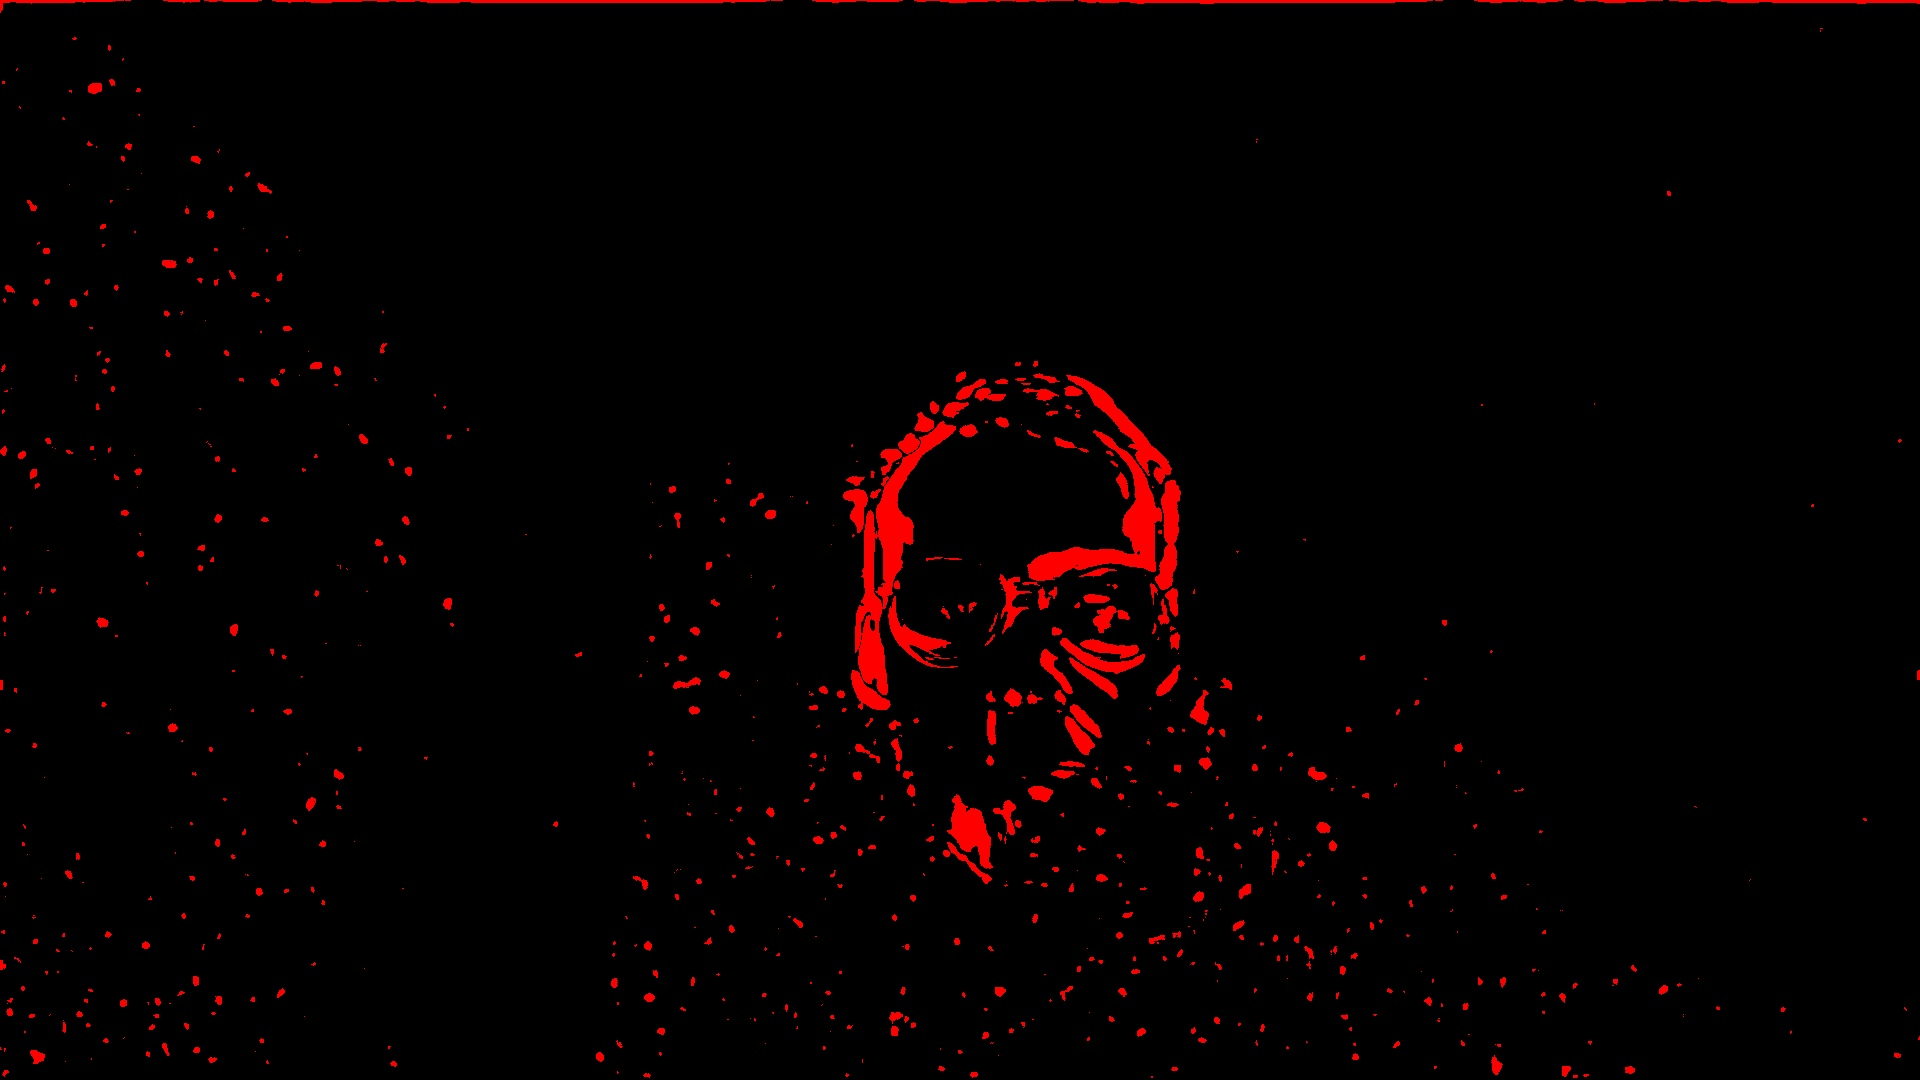
\includegraphics[width=\linewidth]{images/heatmap/img_mean/img_man_red9.jpg}
			\caption{$K=9$}
	\end{subfigure}
		
		\caption{Mean filtering results}
		\label{fig:mean_filter}
	\end{figure}

	\begin{figure}[H]
	\centering
	\begin{subfigure}{0.2\textwidth}
		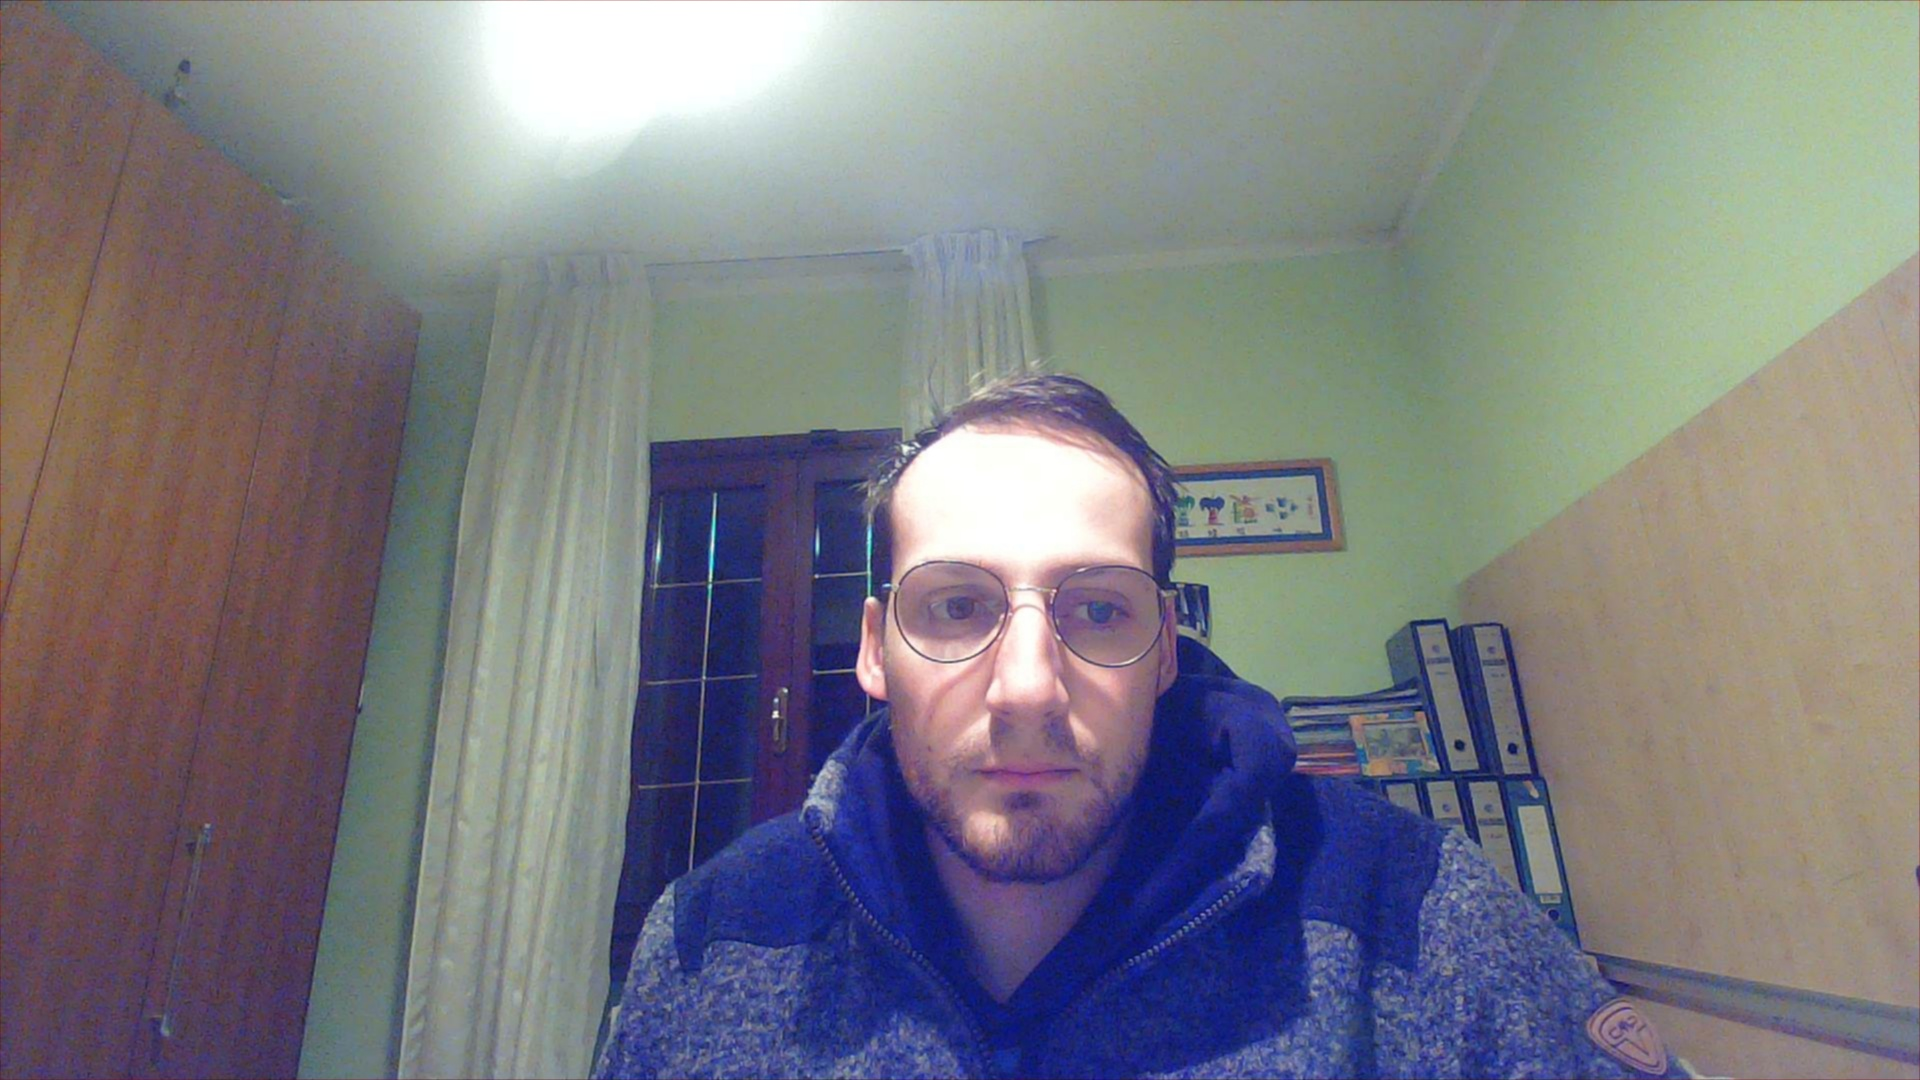
\includegraphics[width=\linewidth]{images/heatmap/img_gaus/img_man_g3.jpg}
	\end{subfigure}%
	\begin{subfigure}{0.2\textwidth}
		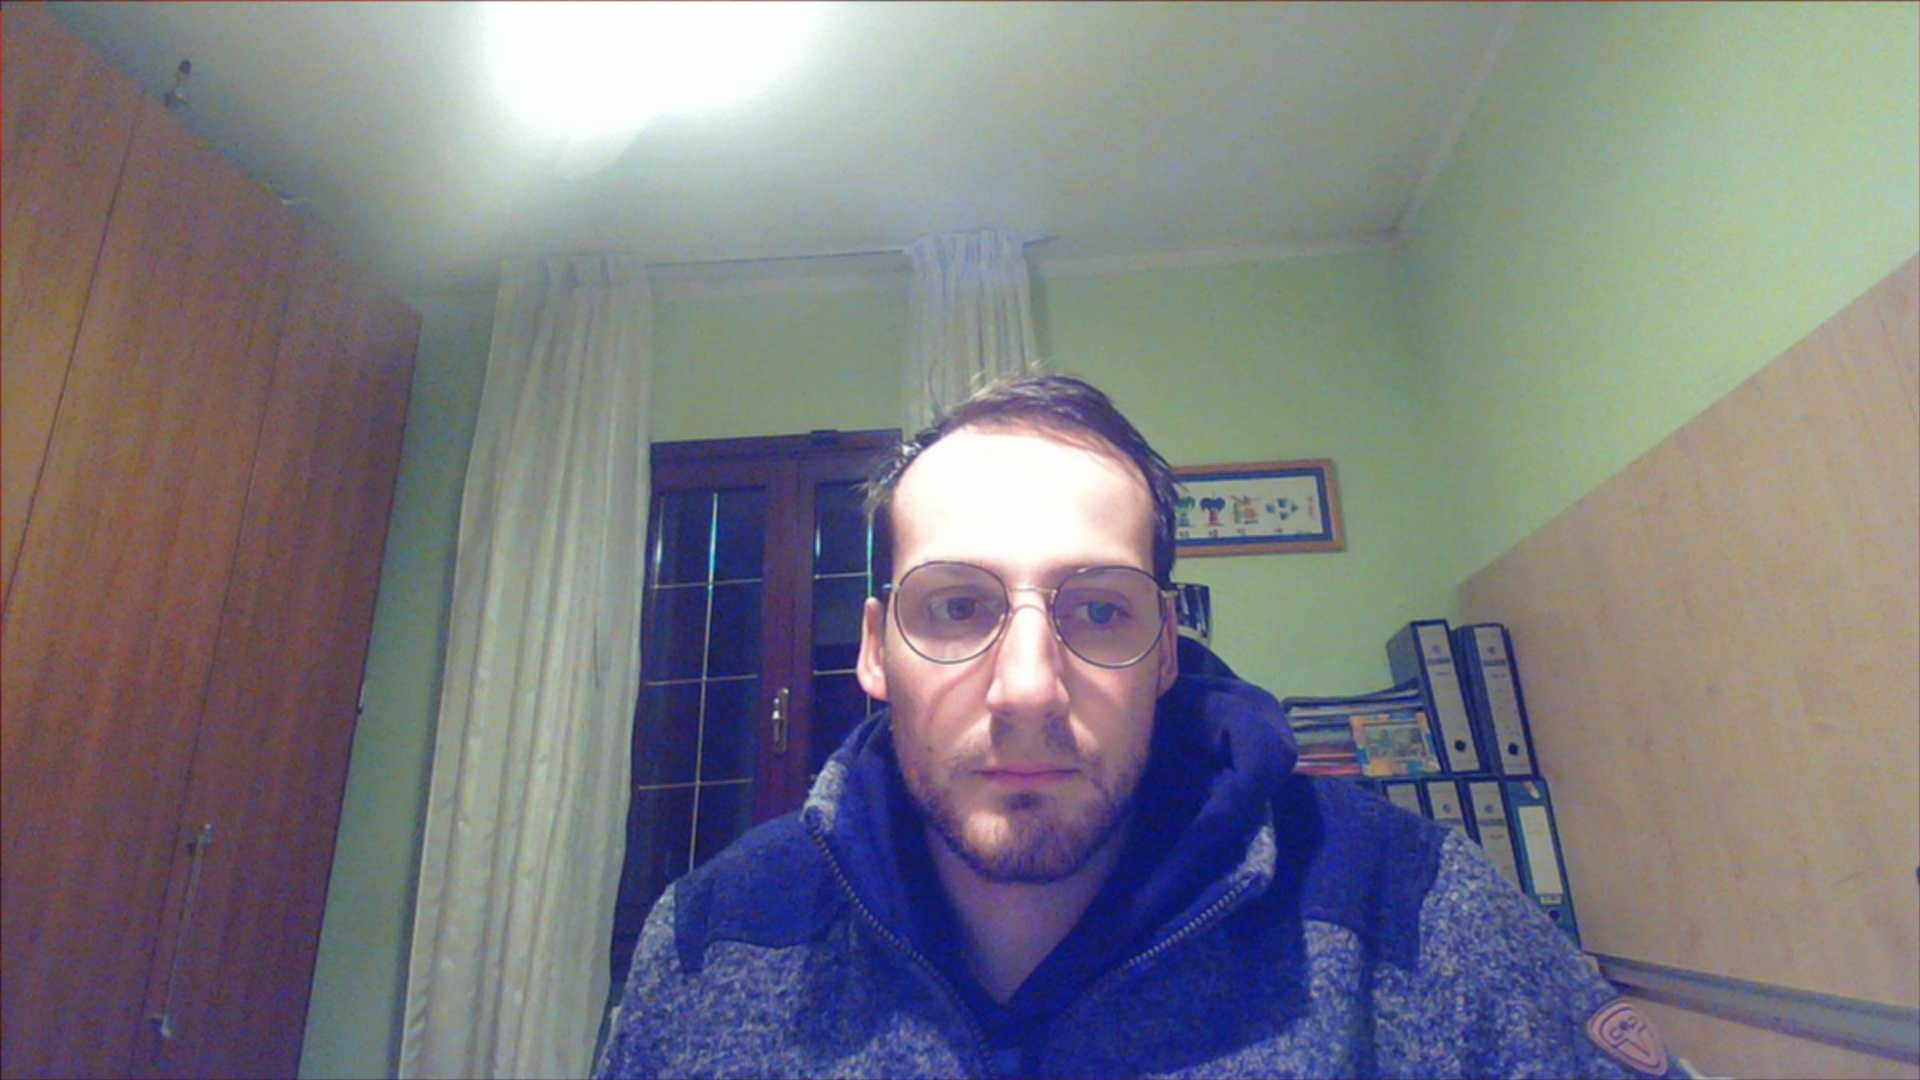
\includegraphics[width=\linewidth]{images/heatmap/img_gaus/img_man_g4.jpg}
	\end{subfigure}%
	\begin{subfigure}{0.2\textwidth}
		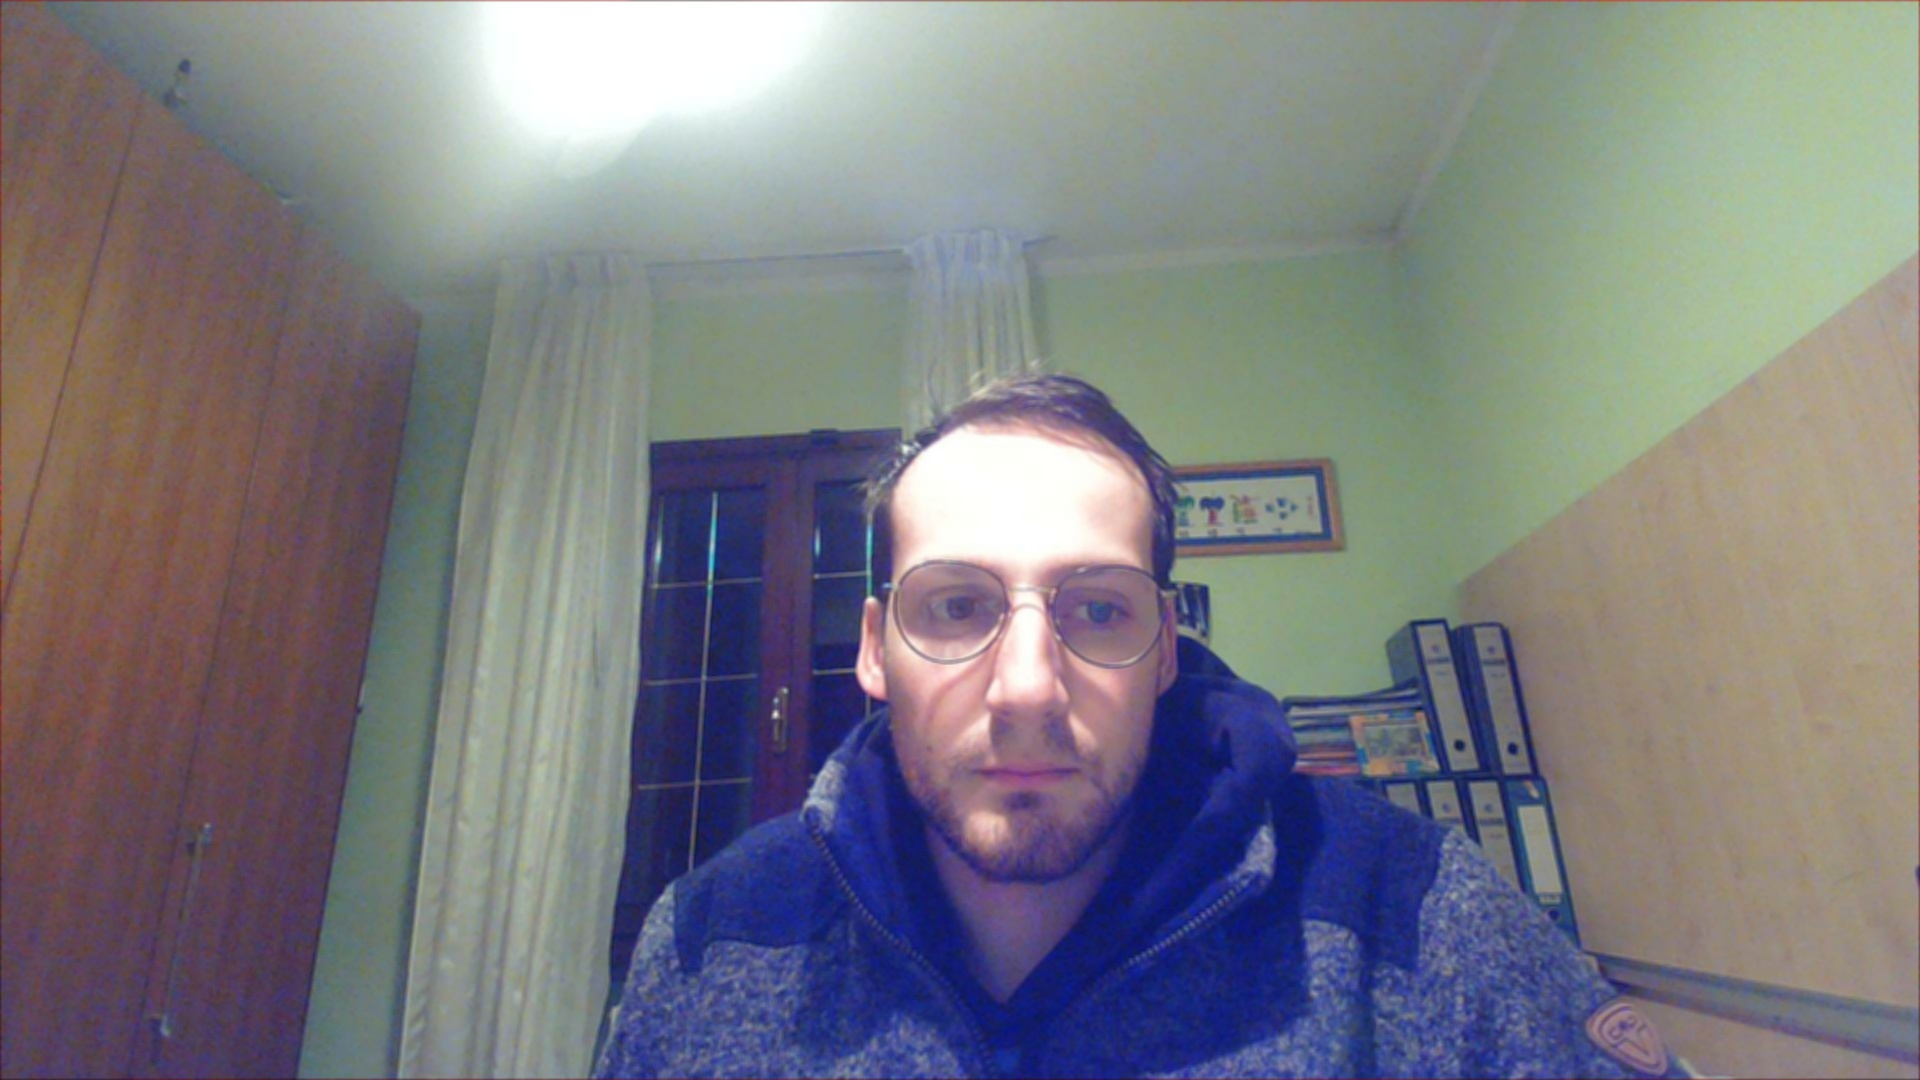
\includegraphics[width=\linewidth]{images/heatmap/img_gaus/img_man_g5.jpg}
	\end{subfigure}%
	\begin{subfigure}{0.2\textwidth}
		\includegraphics[width=\linewidth]{images/heatmap/img_gaus/img_man_g6.jpg}
	\end{subfigure}%
	\begin{subfigure}{0.2\textwidth}
		\includegraphics[width=\linewidth]{images/heatmap/img_gaus/img_man_g7.jpg}
	\end{subfigure}
	\begin{subfigure}{0.2\textwidth}
		\includegraphics[width=\linewidth]{images/heatmap/img_gaus/img_man_red_g3.jpg}
		\caption{$K=3$}
	\end{subfigure}%
	\begin{subfigure}{0.2\textwidth}
		\includegraphics[width=\linewidth]{images/heatmap/img_gaus/img_man_red_g4.jpg}
		\caption{$K=4$}
	\end{subfigure}%
	\begin{subfigure}{0.2\textwidth}
		\includegraphics[width=\linewidth]{images/heatmap/img_gaus/img_man_red_g5.jpg}
		\caption{$K=5$}
	\end{subfigure}%
	\begin{subfigure}{0.2\textwidth}
		\includegraphics[width=\linewidth]{images/heatmap/img_gaus/img_man_red_g6.jpg}
		\caption{$K=6$}
	\end{subfigure}%
	\begin{subfigure}{0.2\textwidth}
		\includegraphics[width=\linewidth]{images/heatmap/img_gaus/img_man_red_g7.jpg}
		\caption{$K=7$}
	\end{subfigure}
	
	\caption{Gaussian filtering results}
	\label{fig:gaus_filter}
	\end{figure}
	
	By visually inspecting the results, by using a kernel that is too large, leads to a non-negligible distortion to the image due to the blur effect. By the way, the team has defined that the best visual result is when $K=4$, using the Gaussian Filter, that allows to avoid to send about 10600 pixels, with the respect to the selected two frames.

	\subsection{2D CUDA Tiled Median filter}
	Another algorithm that has been selected to try to remove the noise from the image is the Medial filter. It works in a completely different way from the Mean and Gaussian filters. The idea behind of it is to preserve the useful details of the image while removing the noise.
	
	Like the Mean filter, the Median one takes $N$ neighbor pixels that are next to the selected one but, instead of replacing it with the average value between all of them it replace that pixel with the \textit{median}.\newline\newline
	The median of a plan one dimensional array can be computed by first sorting all elements and then take the one in the middle of the array itself. On the other hand, if we have a matrix, the media con be computed in the same way, but all elements are considered and ordered.
	\begin{table}[H]
		\centering
		\begin{tabular}{ |c:c:c| } 
			\hline
			1 & 7 & 3 \\
			\hdashline
			2 & \textbf{9} & 6 \\ 
			\hdashline
			4 & 1 & 6 \\ 
			\hline
		\end{tabular}
		$\implies$ [1, 1, 2, 3, \textbf{4}, 6, 6, 7, 9] $\implies$ 4
		\caption{\textit{Median of a matrix 3x3}}
		\label{tab:median_matrix}
	\end{table}
	In this case, the example above shows the media computation of a matrix 3x3 that can corresponds to the kernel size of CUDA kernel.\newline\newline
	The CUDA algorithm is structured in the same way as the convolution one, in which the image processing is divided into \textit{tiles} of fixed dimensions. In the same way, pixels are loaded into the shared memory in order to reduce the accesses to the Global memory.
	
	So, the first step to do is to generate a CUDA function that is able to extract the media from a given array, of size $K*K$. The following code shows the implementation of the Bubble Sort and take the median element, by assuming that $N$ is odd:
	\begin{lstlisting}[style=CStyle]
__device__ uint8_t median(uint8_t *array, int N){
	bool swapped = true;
	for (int a = 0; a < N && swapped; a++){
		swapped = false;
		for (int i = 0; i < N - 1; i++){
			if(array[i] > array[i+1]){
				uint8_t tmp = array[i];
				array[i] = array[i+1];
				array[i+1] = tmp;
				swapped = true;
			}
		}
	}
	
	return array[N/2];
}\end{lstlisting}

	At this point, the kernel must load into the shared memory the image and then, foreach thread three arrays are computed; one for each of the color components. By iterating of the tile, elements are put in the three arrays and the median extracted. At this point, the new image is computed using that median. The following code shows the kernel for the media filtering.
	
		\begin{lstlisting}[style=CStyle]
__global__ void median_kernel(uint8_t *image, uint8_t *R)
{
	__shared__ uint8_t N_ds[BLOCK_SIZE][BLOCK_SIZE*3];
	
	int tx = threadIdx.x;   //W
	int ty = threadIdx.y;   //H
	int row_o = blockIdx.y*TILE_SIZE + ty;
	int col_o = blockIdx.x*TILE_SIZE + tx;
	int row_i = row_o - K/2;
	int col_i = col_o - K/2;
	
	if(row_i >= 0 && row_i < H && col_i >= 0 && col_i < W){
		N_ds[ty][tx*3] = image[row_i*W*3+ col_i * C];
		N_ds[ty][tx*3+1] = image[row_i*W*3+ col_i*3 + 1 ];
		N_ds[ty][tx*3+2] = image[row_i*W*3+ col_i*3 + 2 ];
	} else {
		N_ds[ty][tx*3] = 0;
		N_ds[ty][tx*3+1] = 0;
		N_ds[ty][tx*3+1] = 0;
	}
	
	__syncthreads();
	
	if(row_o < H && col_o < W && ty < TILE_SIZE && tx < TILE_SIZE){
		uint8_t medR[K*K];
		uint8_t medG[K*K];
		uint8_t medB[K*K];
		int r = 0;
		int g = 0;
		int b = 0;
		
		// Copying elements into the three arrays
		for(int i = 0; i < K; i++)
			for(int j = 0; j < K; j++){
				medR[r++] = N_ds[i+ty][(j+tx)*3];
				medG[g++] = N_ds[i+ty][(j+tx)*3 + 1];
				medB[b++] = N_ds[i+ty][(j+tx)*3 + 2];
			}
		
		// Computation of the median
		R[row_o*W*3 + col_o*3] = median(medR, K*K);
		R[row_o*W*3 + col_o*3 + 1] = median(medG, K*K);
		R[row_o*W*3 + col_o*3 + 2] = median(medB, K*K);
	}
}\end{lstlisting}
	
	The problem with this implementation is that, it needs to sort an array of $K*K$ elements for each color component in the image, that obviously implies a longer computation. The below images are from the execution of the above algorithm, using $K=5$ and a frame of 1920*1080*3 elements. The kernel execution time from the \textit{profiler} is 574.67ms, that is a lot if we want to keep the FPS sufficiently high.
	
		
	\begin{figure}[H]
		\centering
		\begin{minipage}[b]{0.45\textwidth}
			\centering
			\includegraphics[width=0.85\textwidth]{images/heatmap/img_median_or.jpg}
			\caption{\textit{Median filtered frame}}
		\end{minipage}
		\hfill
		\begin{minipage}[b]{0.45\textwidth}
			\centering
			\includegraphics[width=0.85\textwidth]{images/heatmap/img_median_red.jpg}
			\caption{\textit{Red-black noise visualization}}
		\end{minipage}
		\caption{\textit{Example of Median filter with $K = 5$}}
	\end{figure}

	Let's suppose for a moment that we do not have any constraint from the FPS; \textit{is it a good solution for the noise?} From the point of view of the percentage of the total pixels saved, we have only 2.54\%, that is even higher the result from a simpler Mean filter with the same kernel size.
	
	The problem with this filter is comping from the type of noise that is characterizing out frames. In fact, the Median filter works better on \textit{Salt and Pepper} noise, that are some random pixels that have completely different values from the point of view of the magnitude. Let's see an example:
	\begin{table}[H]
		\centering
		\begin{tabular}{ |c:c:c| } 
			\hline
			1 & 7 & 3 \\
			\hdashline
			2 & \textbf{89} & 6 \\ 
			\hdashline
			4 & 1 & 6 \\ 
			\hline
		\end{tabular}
		$\implies$ [1, 1, 2, 3, \textbf{4}, 6, 6, 7, 89] $\implies$ 4
		\caption{\textit{Median of a matrix 3x3, with salt and pepper noise}}
		\label{tab:median_matrix_work}
	\end{table}
	\begin{figure}[H]
		\centering
		\includegraphics[width=0.26\linewidth]{images/heatmap/salt_and_pepper_noise}
		\caption{\textit{Salt and pepper noise}}
		\label{fig:saltandpeppernoise}
	\end{figure}

	So, due to the fact that the Median filter does not bring any advantage, it has not been optimized and even used. Beside this, the implementation allowed us to better understand the nature of the noise.

\end{document}
